\documentclass[twoside]{book}

% Packages required by doxygen
\usepackage{calc}
\usepackage{doxygen}
\usepackage{graphicx}
\usepackage[utf8]{inputenc}
\usepackage{makeidx}
\usepackage{multicol}
\usepackage{multirow}
\usepackage{textcomp}
\usepackage[table]{xcolor}

% Font selection
\usepackage[T1]{fontenc}
\usepackage{mathptmx}
\usepackage[scaled=.90]{helvet}
\usepackage{courier}
\usepackage{amssymb}
\usepackage{sectsty}
\renewcommand{\familydefault}{\sfdefault}
\allsectionsfont{%
  \fontseries{bc}\selectfont%
  \color{darkgray}%
}
\renewcommand{\DoxyLabelFont}{%
  \fontseries{bc}\selectfont%
  \color{darkgray}%
}

% Page & text layout
\usepackage{geometry}
\geometry{%
  a4paper,%
  top=2.5cm,%
  bottom=2.5cm,%
  left=2.5cm,%
  right=2.5cm%
}
\tolerance=750
\hfuzz=15pt
\hbadness=750
\setlength{\emergencystretch}{15pt}
\setlength{\parindent}{0cm}
\setlength{\parskip}{0.2cm}
\makeatletter
\renewcommand{\paragraph}{%
  \@startsection{paragraph}{4}{0ex}{-1.0ex}{1.0ex}{%
    \normalfont\normalsize\bfseries\SS@parafont%
  }%
}
\renewcommand{\subparagraph}{%
  \@startsection{subparagraph}{5}{0ex}{-1.0ex}{1.0ex}{%
    \normalfont\normalsize\bfseries\SS@subparafont%
  }%
}
\makeatother

% Headers & footers
\usepackage{fancyhdr}
\pagestyle{fancyplain}
\fancyhead[LE]{\fancyplain{}{\bfseries\thepage}}
\fancyhead[CE]{\fancyplain{}{}}
\fancyhead[RE]{\fancyplain{}{\bfseries\leftmark}}
\fancyhead[LO]{\fancyplain{}{\bfseries\rightmark}}
\fancyhead[CO]{\fancyplain{}{}}
\fancyhead[RO]{\fancyplain{}{\bfseries\thepage}}
\fancyfoot[LE]{\fancyplain{}{}}
\fancyfoot[CE]{\fancyplain{}{}}
\fancyfoot[RE]{\fancyplain{}{\bfseries\scriptsize Generated on Tue Apr 28 2015 20\-:46\-:53 for Nate's E\-T\-L by Doxygen }}
\fancyfoot[LO]{\fancyplain{}{\bfseries\scriptsize Generated on Tue Apr 28 2015 20\-:46\-:53 for Nate's E\-T\-L by Doxygen }}
\fancyfoot[CO]{\fancyplain{}{}}
\fancyfoot[RO]{\fancyplain{}{}}
\renewcommand{\footrulewidth}{0.4pt}
\renewcommand{\chaptermark}[1]{%
  \markboth{#1}{}%
}
\renewcommand{\sectionmark}[1]{%
  \markright{\thesection\ #1}%
}

% Indices & bibliography
\usepackage{natbib}
\usepackage[titles]{tocloft}
\setcounter{tocdepth}{3}
\setcounter{secnumdepth}{5}
\makeindex

% Hyperlinks (required, but should be loaded last)
\usepackage{ifpdf}
\ifpdf
  \usepackage[pdftex,pagebackref=true]{hyperref}
\else
  \usepackage[ps2pdf,pagebackref=true]{hyperref}
\fi
\hypersetup{%
  colorlinks=true,%
  linkcolor=blue,%
  citecolor=blue,%
  unicode%
}

% Custom commands
\newcommand{\clearemptydoublepage}{%
  \newpage{\pagestyle{empty}\cleardoublepage}%
}


%===== C O N T E N T S =====

\begin{document}

% Titlepage & ToC
\hypersetup{pageanchor=false}
\pagenumbering{roman}
\begin{titlepage}
\vspace*{7cm}
\begin{center}%
{\Large Nate's E\-T\-L }\\
\vspace*{1cm}
{\large Generated by Doxygen 1.8.6}\\
\vspace*{0.5cm}
{\small Tue Apr 28 2015 20:46:53}\\
\end{center}
\end{titlepage}
\clearemptydoublepage
\tableofcontents
\clearemptydoublepage
\pagenumbering{arabic}
\hypersetup{pageanchor=true}

%--- Begin generated contents ---
\chapter{Namespace Index}
\section{Namespace List}
Here is a list of all documented namespaces with brief descriptions\-:\begin{DoxyCompactList}
\item\contentsline{section}{\hyperlink{namespaceetl_1_1common}{etl.\-common} }{\pageref{namespaceetl_1_1common}}{}
\item\contentsline{section}{\hyperlink{namespaceetl_1_1EtlJoinProcessor}{etl.\-Etl\-Join\-Processor} }{\pageref{namespaceetl_1_1EtlJoinProcessor}}{}
\item\contentsline{section}{\hyperlink{namespaceetl_1_1EtlProcessor}{etl.\-Etl\-Processor} }{\pageref{namespaceetl_1_1EtlProcessor}}{}
\item\contentsline{section}{\hyperlink{namespaceetl_1_1EtlRecord}{etl.\-Etl\-Record} }{\pageref{namespaceetl_1_1EtlRecord}}{}
\item\contentsline{section}{\hyperlink{namespaceetl_1_1EtlWorkflow}{etl.\-Etl\-Workflow} }{\pageref{namespaceetl_1_1EtlWorkflow}}{}
\item\contentsline{section}{\hyperlink{namespaceetl_1_1exceptions}{etl.\-exceptions} }{\pageref{namespaceetl_1_1exceptions}}{}
\item\contentsline{section}{\hyperlink{namespaceetl_1_1schema}{etl.\-schema} }{\pageref{namespaceetl_1_1schema}}{}
\item\contentsline{section}{\hyperlink{namespaceetl_1_1schema_1_1EtlSchema}{etl.\-schema.\-Etl\-Schema} }{\pageref{namespaceetl_1_1schema_1_1EtlSchema}}{}
\item\contentsline{section}{\hyperlink{namespaceetl_1_1tk__monitor_1_1PrcStatusGridComponents}{etl.\-tk\-\_\-monitor.\-Prc\-Status\-Grid\-Components} }{\pageref{namespaceetl_1_1tk__monitor_1_1PrcStatusGridComponents}}{}
\end{DoxyCompactList}

\chapter{Hierarchical Index}
\section{Class Hierarchy}
This inheritance list is sorted roughly, but not completely, alphabetically\-:\begin{DoxyCompactList}
\item Exception\begin{DoxyCompactList}
\item \contentsline{section}{etl.\-Etl\-Record.\-Etl\-Record\-Frozen}{\pageref{classetl_1_1EtlRecord_1_1EtlRecordFrozen}}{}
\item \contentsline{section}{etl.\-exceptions.\-Etl\-Build\-Error}{\pageref{classetl_1_1exceptions_1_1EtlBuildError}}{}
\begin{DoxyCompactList}
\item \contentsline{section}{etl.\-exceptions.\-Invalid\-Data\-Port\-Name}{\pageref{classetl_1_1exceptions_1_1InvalidDataPortName}}{}
\item \contentsline{section}{etl.\-exceptions.\-Invalid\-Processor\-Name}{\pageref{classetl_1_1exceptions_1_1InvalidProcessorName}}{}
\end{DoxyCompactList}
\end{DoxyCompactList}
\item object\begin{DoxyCompactList}
\item \contentsline{section}{etl.\-Etl\-Event.\-Etl\-Event}{\pageref{classetl_1_1EtlEvent_1_1EtlEvent}}{}
\begin{DoxyCompactList}
\item \contentsline{section}{etl.\-Etl\-Event.\-Input\-Record\-Recieved}{\pageref{classetl_1_1EtlEvent_1_1InputRecordRecieved}}{}
\item \contentsline{section}{etl.\-Etl\-Event.\-Prc\-Disconnected\-Event}{\pageref{classetl_1_1EtlEvent_1_1PrcDisconnectedEvent}}{}
\end{DoxyCompactList}
\item \contentsline{section}{etl.\-Etl\-Processor.\-Etl\-Processor\-Data\-Port}{\pageref{classetl_1_1EtlProcessor_1_1EtlProcessorDataPort}}{}
\item \contentsline{section}{etl.\-Etl\-Processor\-Base.\-Etl\-Processor\-Base}{\pageref{classetl_1_1EtlProcessorBase_1_1EtlProcessorBase}}{}
\item \contentsline{section}{etl.\-Etl\-Record.\-Etl\-Record\-Serial}{\pageref{classetl_1_1EtlRecord_1_1EtlRecordSerial}}{}
\item \contentsline{section}{etl.\-Etl\-Record\-Set.\-Etl\-Record\-Set}{\pageref{classetl_1_1EtlRecordSet_1_1EtlRecordSet}}{}
\item \contentsline{section}{etl.\-ports.\-Etl\-Input\-Connection}{\pageref{classetl_1_1ports_1_1EtlInputConnection}}{}
\item \contentsline{section}{etl.\-ports.\-Etl\-Output\-Connection}{\pageref{classetl_1_1ports_1_1EtlOutputConnection}}{}
\item \contentsline{section}{etl.\-ports.\-Port\-Base}{\pageref{classetl_1_1ports_1_1PortBase}}{}
\begin{DoxyCompactList}
\item \contentsline{section}{etl.\-ports.\-Input\-Port}{\pageref{classetl_1_1ports_1_1InputPort}}{}
\item \contentsline{section}{etl.\-ports.\-Output\-Port}{\pageref{classetl_1_1ports_1_1OutputPort}}{}
\end{DoxyCompactList}
\item \contentsline{section}{etl.\-ports.\-Port\-Collection}{\pageref{classetl_1_1ports_1_1PortCollection}}{}
\begin{DoxyCompactList}
\item \contentsline{section}{etl.\-ports.\-Input\-Port\-Collection}{\pageref{classetl_1_1ports_1_1InputPortCollection}}{}
\item \contentsline{section}{etl.\-ports.\-Output\-Port\-Collection}{\pageref{classetl_1_1ports_1_1OutputPortCollection}}{}
\end{DoxyCompactList}
\item \contentsline{section}{etl.\-Post\-Record\-Processing\-Action.\-Post\-Record\-Processing\-Action}{\pageref{classetl_1_1PostRecordProcessingAction_1_1PostRecordProcessingAction}}{}
\begin{DoxyCompactList}
\item \contentsline{section}{etl.\-Post\-Record\-Processing\-Action.\-Get\-Next\-Input\-Record}{\pageref{classetl_1_1PostRecordProcessingAction_1_1GetNextInputRecord}}{}
\item \contentsline{section}{etl.\-Post\-Record\-Processing\-Action.\-Hold\-Record}{\pageref{classetl_1_1PostRecordProcessingAction_1_1HoldRecord}}{}
\item \contentsline{section}{etl.\-Post\-Record\-Processing\-Action.\-Record\-Consumed}{\pageref{classetl_1_1PostRecordProcessingAction_1_1RecordConsumed}}{}
\end{DoxyCompactList}
\item \contentsline{section}{etl.\-recshelf.\-Memory\-Record\-Set.\-Memory\-Record\-Set}{\pageref{classetl_1_1recshelf_1_1MemoryRecordSet_1_1MemoryRecordSet}}{}
\item \contentsline{section}{etl.\-recshelf.\-Record\-Shelf.\-Record\-Shelf}{\pageref{classetl_1_1recshelf_1_1RecordShelf_1_1RecordShelf}}{}
\item \contentsline{section}{etl.\-recshelf.\-Sqlite3\-Record\-Set.\-Sqlite3\-Record\-Set}{\pageref{classetl_1_1recshelf_1_1Sqlite3RecordSet_1_1Sqlite3RecordSet}}{}
\item \contentsline{section}{etl.\-schema.\-Etl\-Schema.\-Etl\-Schema}{\pageref{classetl_1_1schema_1_1EtlSchema_1_1EtlSchema}}{}
\item \contentsline{section}{etl.\-schema.\-Etl\-Schema\-Element.\-Etl\-Schema\-Element}{\pageref{classetl_1_1schema_1_1EtlSchemaElement_1_1EtlSchemaElement}}{}
\item \contentsline{section}{etl.\-tk\-\_\-monitor.\-Prc\-Status\-Grid\-Components.\-Prc\-Status\-Grid\-Component}{\pageref{classetl_1_1tk__monitor_1_1PrcStatusGridComponents_1_1PrcStatusGridComponent}}{}
\begin{DoxyCompactList}
\item \contentsline{section}{etl.\-tk\-\_\-monitor.\-Prc\-Status\-Grid\-Components.\-Data\-Port\-In\-Grid}{\pageref{classetl_1_1tk__monitor_1_1PrcStatusGridComponents_1_1DataPortInGrid}}{}
\item \contentsline{section}{etl.\-tk\-\_\-monitor.\-Prc\-Status\-Grid\-Components.\-Process\-In\-Grid}{\pageref{classetl_1_1tk__monitor_1_1PrcStatusGridComponents_1_1ProcessInGrid}}{}
\end{DoxyCompactList}
\item \contentsline{section}{etl.\-tk\-\_\-monitor.\-Tk\-Workflow\-Monitor.\-Tk\-Workflow\-Monitor}{\pageref{classetl_1_1tk__monitor_1_1TkWorkflowMonitor_1_1TkWorkflowMonitor}}{}
\item \contentsline{section}{etl.\-Workflow\-Data\-Path.\-Workflow\-Data\-Path}{\pageref{classetl_1_1WorkflowDataPath_1_1WorkflowDataPath}}{}
\end{DoxyCompactList}
\item Frame\begin{DoxyCompactList}
\item \contentsline{section}{etl.\-tk\-\_\-monitor.\-Tk\-Scrollable\-Grid.\-Tk\-Scrollable\-Grid}{\pageref{classetl_1_1tk__monitor_1_1TkScrollableGrid_1_1TkScrollableGrid}}{}
\end{DoxyCompactList}
\item Etl\-Processor\begin{DoxyCompactList}
\item \contentsline{section}{etl.\-Etl\-Join\-Processor.\-Etl\-Join\-Processor}{\pageref{classetl_1_1EtlJoinProcessor_1_1EtlJoinProcessor}}{}
\end{DoxyCompactList}
\item Etl\-Processor\-Base\begin{DoxyCompactList}
\item \contentsline{section}{etl.\-Etl\-Processor.\-Etl\-Processor}{\pageref{classetl_1_1EtlProcessor_1_1EtlProcessor}}{}
\begin{DoxyCompactList}
\item \contentsline{section}{etl.\-common.\-Field\-Find\-Replace.\-Field\-Find\-Replace}{\pageref{classetl_1_1common_1_1FieldFindReplace_1_1FieldFindReplace}}{}
\end{DoxyCompactList}
\item \contentsline{section}{etl.\-Etl\-Workflow.\-Etl\-Workflow}{\pageref{classetl_1_1EtlWorkflow_1_1EtlWorkflow}}{}
\end{DoxyCompactList}
\item Etl\-Schema\-Element\begin{DoxyCompactList}
\item \contentsline{section}{etl.\-schema.\-Etl\-Any\-Element.\-Etl\-Any\-Element}{\pageref{classetl_1_1schema_1_1EtlAnyElement_1_1EtlAnyElement}}{}
\item \contentsline{section}{etl.\-schema.\-Etl\-Binary\-Element.\-Etl\-Binary\-Element}{\pageref{classetl_1_1schema_1_1EtlBinaryElement_1_1EtlBinaryElement}}{}
\item \contentsline{section}{etl.\-schema.\-Etl\-Bool\-Element.\-Etl\-Bool\-Element}{\pageref{classetl_1_1schema_1_1EtlBoolElement_1_1EtlBoolElement}}{}
\item \contentsline{section}{etl.\-schema.\-Etl\-Int\-Element.\-Etl\-Int\-Element}{\pageref{classetl_1_1schema_1_1EtlIntElement_1_1EtlIntElement}}{}
\item \contentsline{section}{etl.\-schema.\-Etl\-List\-Element.\-Etl\-List\-Element}{\pageref{classetl_1_1schema_1_1EtlListElement_1_1EtlListElement}}{}
\item \contentsline{section}{etl.\-schema.\-Etl\-Record\-Element.\-Etl\-Record\-Element}{\pageref{classetl_1_1schema_1_1EtlRecordElement_1_1EtlRecordElement}}{}
\item \contentsline{section}{etl.\-schema.\-Etl\-String\-Element.\-Etl\-String\-Element}{\pageref{classetl_1_1schema_1_1EtlStringElement_1_1EtlStringElement}}{}
\end{DoxyCompactList}
\item Tk\-Scrollable\-Grid\begin{DoxyCompactList}
\item \contentsline{section}{etl.\-tk\-\_\-monitor.\-Tk\-Processor\-Status\-Grid.\-Tk\-Processor\-Status\-Grid}{\pageref{classetl_1_1tk__monitor_1_1TkProcessorStatusGrid_1_1TkProcessorStatusGrid}}{}
\end{DoxyCompactList}
\item Dict\-Mixin\begin{DoxyCompactList}
\item \contentsline{section}{etl.\-Etl\-Record.\-Etl\-Record}{\pageref{classetl_1_1EtlRecord_1_1EtlRecord}}{}
\end{DoxyCompactList}
\end{DoxyCompactList}

\chapter{Class Index}
\section{Class List}
Here are the classes, structs, unions and interfaces with brief descriptions\-:\begin{DoxyCompactList}
\item\contentsline{section}{\hyperlink{classetl_1_1common_1_1FieldFindReplace_1_1FieldFindReplace}{etl.\-common.\-Field\-Find\-Replace.\-Field\-Find\-Replace} }{\pageref{classetl_1_1common_1_1FieldFindReplace_1_1FieldFindReplace}}{}
\item\contentsline{section}{\hyperlink{classetl_1_1EtlEvent_1_1EtlEvent}{etl.\-Etl\-Event.\-Etl\-Event} }{\pageref{classetl_1_1EtlEvent_1_1EtlEvent}}{}
\item\contentsline{section}{\hyperlink{classetl_1_1EtlEvent_1_1InputRecordRecieved}{etl.\-Etl\-Event.\-Input\-Record\-Recieved} }{\pageref{classetl_1_1EtlEvent_1_1InputRecordRecieved}}{}
\item\contentsline{section}{\hyperlink{classetl_1_1EtlEvent_1_1PrcDisconnectedEvent}{etl.\-Etl\-Event.\-Prc\-Disconnected\-Event} }{\pageref{classetl_1_1EtlEvent_1_1PrcDisconnectedEvent}}{}
\item\contentsline{section}{\hyperlink{classetl_1_1EtlJoinProcessor_1_1EtlJoinProcessor}{etl.\-Etl\-Join\-Processor.\-Etl\-Join\-Processor} }{\pageref{classetl_1_1EtlJoinProcessor_1_1EtlJoinProcessor}}{}
\item\contentsline{section}{\hyperlink{classetl_1_1EtlProcessor_1_1EtlProcessor}{etl.\-Etl\-Processor.\-Etl\-Processor} }{\pageref{classetl_1_1EtlProcessor_1_1EtlProcessor}}{}
\item\contentsline{section}{\hyperlink{classetl_1_1EtlProcessor_1_1EtlProcessorDataPort}{etl.\-Etl\-Processor.\-Etl\-Processor\-Data\-Port} }{\pageref{classetl_1_1EtlProcessor_1_1EtlProcessorDataPort}}{}
\item\contentsline{section}{\hyperlink{classetl_1_1EtlProcessorBase_1_1EtlProcessorBase}{etl.\-Etl\-Processor\-Base.\-Etl\-Processor\-Base} }{\pageref{classetl_1_1EtlProcessorBase_1_1EtlProcessorBase}}{}
\item\contentsline{section}{\hyperlink{classetl_1_1EtlRecord_1_1EtlRecord}{etl.\-Etl\-Record.\-Etl\-Record} }{\pageref{classetl_1_1EtlRecord_1_1EtlRecord}}{}
\item\contentsline{section}{\hyperlink{classetl_1_1EtlRecord_1_1EtlRecordFrozen}{etl.\-Etl\-Record.\-Etl\-Record\-Frozen} }{\pageref{classetl_1_1EtlRecord_1_1EtlRecordFrozen}}{}
\item\contentsline{section}{\hyperlink{classetl_1_1EtlRecord_1_1EtlRecordSerial}{etl.\-Etl\-Record.\-Etl\-Record\-Serial} }{\pageref{classetl_1_1EtlRecord_1_1EtlRecordSerial}}{}
\item\contentsline{section}{\hyperlink{classetl_1_1EtlRecordSet_1_1EtlRecordSet}{etl.\-Etl\-Record\-Set.\-Etl\-Record\-Set} }{\pageref{classetl_1_1EtlRecordSet_1_1EtlRecordSet}}{}
\item\contentsline{section}{\hyperlink{classetl_1_1EtlWorkflow_1_1EtlWorkflow}{etl.\-Etl\-Workflow.\-Etl\-Workflow} }{\pageref{classetl_1_1EtlWorkflow_1_1EtlWorkflow}}{}
\item\contentsline{section}{\hyperlink{classetl_1_1exceptions_1_1EtlBuildError}{etl.\-exceptions.\-Etl\-Build\-Error} }{\pageref{classetl_1_1exceptions_1_1EtlBuildError}}{}
\item\contentsline{section}{\hyperlink{classetl_1_1exceptions_1_1InvalidDataPortName}{etl.\-exceptions.\-Invalid\-Data\-Port\-Name} }{\pageref{classetl_1_1exceptions_1_1InvalidDataPortName}}{}
\item\contentsline{section}{\hyperlink{classetl_1_1exceptions_1_1InvalidProcessorName}{etl.\-exceptions.\-Invalid\-Processor\-Name} }{\pageref{classetl_1_1exceptions_1_1InvalidProcessorName}}{}
\item\contentsline{section}{\hyperlink{classetl_1_1ports_1_1EtlInputConnection}{etl.\-ports.\-Etl\-Input\-Connection} }{\pageref{classetl_1_1ports_1_1EtlInputConnection}}{}
\item\contentsline{section}{\hyperlink{classetl_1_1ports_1_1EtlOutputConnection}{etl.\-ports.\-Etl\-Output\-Connection} }{\pageref{classetl_1_1ports_1_1EtlOutputConnection}}{}
\item\contentsline{section}{\hyperlink{classetl_1_1ports_1_1InputPort}{etl.\-ports.\-Input\-Port} }{\pageref{classetl_1_1ports_1_1InputPort}}{}
\item\contentsline{section}{\hyperlink{classetl_1_1ports_1_1InputPortCollection}{etl.\-ports.\-Input\-Port\-Collection} }{\pageref{classetl_1_1ports_1_1InputPortCollection}}{}
\item\contentsline{section}{\hyperlink{classetl_1_1ports_1_1OutputPort}{etl.\-ports.\-Output\-Port} }{\pageref{classetl_1_1ports_1_1OutputPort}}{}
\item\contentsline{section}{\hyperlink{classetl_1_1ports_1_1OutputPortCollection}{etl.\-ports.\-Output\-Port\-Collection} }{\pageref{classetl_1_1ports_1_1OutputPortCollection}}{}
\item\contentsline{section}{\hyperlink{classetl_1_1ports_1_1PortBase}{etl.\-ports.\-Port\-Base} }{\pageref{classetl_1_1ports_1_1PortBase}}{}
\item\contentsline{section}{\hyperlink{classetl_1_1ports_1_1PortCollection}{etl.\-ports.\-Port\-Collection} }{\pageref{classetl_1_1ports_1_1PortCollection}}{}
\item\contentsline{section}{\hyperlink{classetl_1_1PostRecordProcessingAction_1_1GetNextInputRecord}{etl.\-Post\-Record\-Processing\-Action.\-Get\-Next\-Input\-Record} }{\pageref{classetl_1_1PostRecordProcessingAction_1_1GetNextInputRecord}}{}
\item\contentsline{section}{\hyperlink{classetl_1_1PostRecordProcessingAction_1_1HoldRecord}{etl.\-Post\-Record\-Processing\-Action.\-Hold\-Record} }{\pageref{classetl_1_1PostRecordProcessingAction_1_1HoldRecord}}{}
\item\contentsline{section}{\hyperlink{classetl_1_1PostRecordProcessingAction_1_1PostRecordProcessingAction}{etl.\-Post\-Record\-Processing\-Action.\-Post\-Record\-Processing\-Action} }{\pageref{classetl_1_1PostRecordProcessingAction_1_1PostRecordProcessingAction}}{}
\item\contentsline{section}{\hyperlink{classetl_1_1PostRecordProcessingAction_1_1RecordConsumed}{etl.\-Post\-Record\-Processing\-Action.\-Record\-Consumed} }{\pageref{classetl_1_1PostRecordProcessingAction_1_1RecordConsumed}}{}
\item\contentsline{section}{\hyperlink{classetl_1_1recshelf_1_1MemoryRecordSet_1_1MemoryRecordSet}{etl.\-recshelf.\-Memory\-Record\-Set.\-Memory\-Record\-Set} }{\pageref{classetl_1_1recshelf_1_1MemoryRecordSet_1_1MemoryRecordSet}}{}
\item\contentsline{section}{\hyperlink{classetl_1_1recshelf_1_1RecordShelf_1_1RecordShelf}{etl.\-recshelf.\-Record\-Shelf.\-Record\-Shelf} }{\pageref{classetl_1_1recshelf_1_1RecordShelf_1_1RecordShelf}}{}
\item\contentsline{section}{\hyperlink{classetl_1_1recshelf_1_1Sqlite3RecordSet_1_1Sqlite3RecordSet}{etl.\-recshelf.\-Sqlite3\-Record\-Set.\-Sqlite3\-Record\-Set} }{\pageref{classetl_1_1recshelf_1_1Sqlite3RecordSet_1_1Sqlite3RecordSet}}{}
\item\contentsline{section}{\hyperlink{classetl_1_1schema_1_1EtlAnyElement_1_1EtlAnyElement}{etl.\-schema.\-Etl\-Any\-Element.\-Etl\-Any\-Element} }{\pageref{classetl_1_1schema_1_1EtlAnyElement_1_1EtlAnyElement}}{}
\item\contentsline{section}{\hyperlink{classetl_1_1schema_1_1EtlBinaryElement_1_1EtlBinaryElement}{etl.\-schema.\-Etl\-Binary\-Element.\-Etl\-Binary\-Element} }{\pageref{classetl_1_1schema_1_1EtlBinaryElement_1_1EtlBinaryElement}}{}
\item\contentsline{section}{\hyperlink{classetl_1_1schema_1_1EtlBoolElement_1_1EtlBoolElement}{etl.\-schema.\-Etl\-Bool\-Element.\-Etl\-Bool\-Element} }{\pageref{classetl_1_1schema_1_1EtlBoolElement_1_1EtlBoolElement}}{}
\item\contentsline{section}{\hyperlink{classetl_1_1schema_1_1EtlIntElement_1_1EtlIntElement}{etl.\-schema.\-Etl\-Int\-Element.\-Etl\-Int\-Element} }{\pageref{classetl_1_1schema_1_1EtlIntElement_1_1EtlIntElement}}{}
\item\contentsline{section}{\hyperlink{classetl_1_1schema_1_1EtlListElement_1_1EtlListElement}{etl.\-schema.\-Etl\-List\-Element.\-Etl\-List\-Element} }{\pageref{classetl_1_1schema_1_1EtlListElement_1_1EtlListElement}}{}
\item\contentsline{section}{\hyperlink{classetl_1_1schema_1_1EtlRecordElement_1_1EtlRecordElement}{etl.\-schema.\-Etl\-Record\-Element.\-Etl\-Record\-Element} }{\pageref{classetl_1_1schema_1_1EtlRecordElement_1_1EtlRecordElement}}{}
\item\contentsline{section}{\hyperlink{classetl_1_1schema_1_1EtlSchema_1_1EtlSchema}{etl.\-schema.\-Etl\-Schema.\-Etl\-Schema} }{\pageref{classetl_1_1schema_1_1EtlSchema_1_1EtlSchema}}{}
\item\contentsline{section}{\hyperlink{classetl_1_1schema_1_1EtlSchemaElement_1_1EtlSchemaElement}{etl.\-schema.\-Etl\-Schema\-Element.\-Etl\-Schema\-Element} }{\pageref{classetl_1_1schema_1_1EtlSchemaElement_1_1EtlSchemaElement}}{}
\item\contentsline{section}{\hyperlink{classetl_1_1schema_1_1EtlStringElement_1_1EtlStringElement}{etl.\-schema.\-Etl\-String\-Element.\-Etl\-String\-Element} }{\pageref{classetl_1_1schema_1_1EtlStringElement_1_1EtlStringElement}}{}
\item\contentsline{section}{\hyperlink{classetl_1_1tk__monitor_1_1PrcStatusGridComponents_1_1DataPortInGrid}{etl.\-tk\-\_\-monitor.\-Prc\-Status\-Grid\-Components.\-Data\-Port\-In\-Grid} }{\pageref{classetl_1_1tk__monitor_1_1PrcStatusGridComponents_1_1DataPortInGrid}}{}
\item\contentsline{section}{\hyperlink{classetl_1_1tk__monitor_1_1PrcStatusGridComponents_1_1PrcStatusGridComponent}{etl.\-tk\-\_\-monitor.\-Prc\-Status\-Grid\-Components.\-Prc\-Status\-Grid\-Component} }{\pageref{classetl_1_1tk__monitor_1_1PrcStatusGridComponents_1_1PrcStatusGridComponent}}{}
\item\contentsline{section}{\hyperlink{classetl_1_1tk__monitor_1_1PrcStatusGridComponents_1_1ProcessInGrid}{etl.\-tk\-\_\-monitor.\-Prc\-Status\-Grid\-Components.\-Process\-In\-Grid} }{\pageref{classetl_1_1tk__monitor_1_1PrcStatusGridComponents_1_1ProcessInGrid}}{}
\item\contentsline{section}{\hyperlink{classetl_1_1tk__monitor_1_1TkProcessorStatusGrid_1_1TkProcessorStatusGrid}{etl.\-tk\-\_\-monitor.\-Tk\-Processor\-Status\-Grid.\-Tk\-Processor\-Status\-Grid} }{\pageref{classetl_1_1tk__monitor_1_1TkProcessorStatusGrid_1_1TkProcessorStatusGrid}}{}
\item\contentsline{section}{\hyperlink{classetl_1_1tk__monitor_1_1TkScrollableGrid_1_1TkScrollableGrid}{etl.\-tk\-\_\-monitor.\-Tk\-Scrollable\-Grid.\-Tk\-Scrollable\-Grid} }{\pageref{classetl_1_1tk__monitor_1_1TkScrollableGrid_1_1TkScrollableGrid}}{}
\item\contentsline{section}{\hyperlink{classetl_1_1tk__monitor_1_1TkWorkflowMonitor_1_1TkWorkflowMonitor}{etl.\-tk\-\_\-monitor.\-Tk\-Workflow\-Monitor.\-Tk\-Workflow\-Monitor} }{\pageref{classetl_1_1tk__monitor_1_1TkWorkflowMonitor_1_1TkWorkflowMonitor}}{}
\item\contentsline{section}{\hyperlink{classetl_1_1WorkflowDataPath_1_1WorkflowDataPath}{etl.\-Workflow\-Data\-Path.\-Workflow\-Data\-Path} }{\pageref{classetl_1_1WorkflowDataPath_1_1WorkflowDataPath}}{}
\end{DoxyCompactList}

\chapter{Namespace Documentation}
\hypertarget{namespaceetl_1_1common}{\section{etl.\-common Namespace Reference}
\label{namespaceetl_1_1common}\index{etl.\-common@{etl.\-common}}
}


\subsection{Detailed Description}
\begin{DoxyVerb}Library of re-usable, generic processors\end{DoxyVerb}
 
\hypertarget{namespaceetl_1_1EtlJoinProcessor}{\section{etl.\-Etl\-Join\-Processor Namespace Reference}
\label{namespaceetl_1_1EtlJoinProcessor}\index{etl.\-Etl\-Join\-Processor@{etl.\-Etl\-Join\-Processor}}
}
\subsection*{Classes}
\begin{DoxyCompactItemize}
\item 
class \hyperlink{classetl_1_1EtlJoinProcessor_1_1EtlJoinProcessor}{Etl\-Join\-Processor}
\end{DoxyCompactItemize}


\subsection{Detailed Description}
\begin{DoxyVerb}Created on Dec 28, 2012

@author: nshearer
\end{DoxyVerb}
 
\hypertarget{namespaceetl_1_1EtlProcessor}{\section{etl.\-Etl\-Processor Namespace Reference}
\label{namespaceetl_1_1EtlProcessor}\index{etl.\-Etl\-Processor@{etl.\-Etl\-Processor}}
}
\subsection*{Classes}
\begin{DoxyCompactItemize}
\item 
class \hyperlink{classetl_1_1EtlProcessor_1_1EtlProcessorDataPort}{Etl\-Processor\-Data\-Port}
\item 
class \hyperlink{classetl_1_1EtlProcessor_1_1EtlProcessor}{Etl\-Processor}
\end{DoxyCompactItemize}


\subsection{Detailed Description}
\begin{DoxyVerb}Created on Dec 27, 2012

@author: nshearer
\end{DoxyVerb}
 
\hypertarget{namespaceetl_1_1EtlRecord}{\section{etl.\-Etl\-Record Namespace Reference}
\label{namespaceetl_1_1EtlRecord}\index{etl.\-Etl\-Record@{etl.\-Etl\-Record}}
}
\subsection*{Classes}
\begin{DoxyCompactItemize}
\item 
class \hyperlink{classetl_1_1EtlRecord_1_1EtlRecordSerial}{Etl\-Record\-Serial}
\item 
class \hyperlink{classetl_1_1EtlRecord_1_1EtlRecordFrozen}{Etl\-Record\-Frozen}
\item 
class \hyperlink{classetl_1_1EtlRecord_1_1EtlRecord}{Etl\-Record}
\end{DoxyCompactItemize}
\subsection*{Variables}
\begin{DoxyCompactItemize}
\item 
\hypertarget{namespaceetl_1_1EtlRecord_a90e10445f0b4332a137ed2716c3d6e00}{int {\bfseries N\-E\-X\-T\-\_\-\-E\-T\-L\-\_\-\-R\-E\-C\-O\-R\-D\-\_\-\-S\-E\-R\-I\-A\-L} = 0\-L}\label{namespaceetl_1_1EtlRecord_a90e10445f0b4332a137ed2716c3d6e00}

\item 
\hypertarget{namespaceetl_1_1EtlRecord_adb345323a14bb22653450d7496e1961d}{tuple {\bfseries N\-E\-X\-T\-\_\-\-E\-T\-L\-\_\-\-R\-E\-C\-O\-R\-D\-\_\-\-L\-O\-C\-K} = Lock()}\label{namespaceetl_1_1EtlRecord_adb345323a14bb22653450d7496e1961d}

\end{DoxyCompactItemize}


\subsection{Detailed Description}
\begin{DoxyVerb}Created on Dec 27, 2012

@author: nshearer
\end{DoxyVerb}
 
\hypertarget{namespaceetl_1_1EtlWorkflow}{\section{etl.\-Etl\-Workflow Namespace Reference}
\label{namespaceetl_1_1EtlWorkflow}\index{etl.\-Etl\-Workflow@{etl.\-Etl\-Workflow}}
}
\subsection*{Classes}
\begin{DoxyCompactItemize}
\item 
class \hyperlink{classetl_1_1EtlWorkflow_1_1EtlWorkflow}{Etl\-Workflow}
\end{DoxyCompactItemize}


\subsection{Detailed Description}
\begin{DoxyVerb}Created on Dec 27, 2012

@author: nshearer
\end{DoxyVerb}
 
\hypertarget{namespaceetl_1_1exceptions}{\section{etl.\-exceptions Namespace Reference}
\label{namespaceetl_1_1exceptions}\index{etl.\-exceptions@{etl.\-exceptions}}
}
\subsection*{Classes}
\begin{DoxyCompactItemize}
\item 
class \hyperlink{classetl_1_1exceptions_1_1EtlBuildError}{Etl\-Build\-Error}
\item 
class \hyperlink{classetl_1_1exceptions_1_1InvalidDataPortName}{Invalid\-Data\-Port\-Name}
\item 
class \hyperlink{classetl_1_1exceptions_1_1InvalidProcessorName}{Invalid\-Processor\-Name}
\end{DoxyCompactItemize}


\subsection{Detailed Description}
\begin{DoxyVerb}Common exceptions for etl library\end{DoxyVerb}
 
\hypertarget{namespaceetl_1_1schema}{\section{etl.\-schema Namespace Reference}
\label{namespaceetl_1_1schema}\index{etl.\-schema@{etl.\-schema}}
}
\subsection*{Namespaces}
\begin{DoxyCompactItemize}
\item 
\hyperlink{namespaceetl_1_1schema_1_1EtlSchema}{Etl\-Schema}
\end{DoxyCompactItemize}


\subsection{Detailed Description}
\begin{DoxyVerb}Schemas describe the structure of records, and how to handle fields\end{DoxyVerb}
 
\hypertarget{namespaceetl_1_1schema_1_1EtlSchema}{\section{etl.\-schema.\-Etl\-Schema Namespace Reference}
\label{namespaceetl_1_1schema_1_1EtlSchema}\index{etl.\-schema.\-Etl\-Schema@{etl.\-schema.\-Etl\-Schema}}
}
\subsection*{Classes}
\begin{DoxyCompactItemize}
\item 
class \hyperlink{classetl_1_1schema_1_1EtlSchema_1_1EtlSchema}{Etl\-Schema}
\end{DoxyCompactItemize}


\subsection{Detailed Description}
\begin{DoxyVerb}Created on Dec 27, 2012

@author: nshearer
\end{DoxyVerb}
 
\hypertarget{namespaceetl_1_1tk__monitor_1_1PrcStatusGridComponents}{\section{etl.\-tk\-\_\-monitor.\-Prc\-Status\-Grid\-Components Namespace Reference}
\label{namespaceetl_1_1tk__monitor_1_1PrcStatusGridComponents}\index{etl.\-tk\-\_\-monitor.\-Prc\-Status\-Grid\-Components@{etl.\-tk\-\_\-monitor.\-Prc\-Status\-Grid\-Components}}
}
\subsection*{Classes}
\begin{DoxyCompactItemize}
\item 
class \hyperlink{classetl_1_1tk__monitor_1_1PrcStatusGridComponents_1_1PrcStatusGridComponent}{Prc\-Status\-Grid\-Component}
\item 
class \hyperlink{classetl_1_1tk__monitor_1_1PrcStatusGridComponents_1_1DataPortInGrid}{Data\-Port\-In\-Grid}
\item 
class \hyperlink{classetl_1_1tk__monitor_1_1PrcStatusGridComponents_1_1ProcessInGrid}{Process\-In\-Grid}
\end{DoxyCompactItemize}


\subsection{Detailed Description}
\begin{DoxyVerb}Created on Apr 16, 2014

@author: nshearer
\end{DoxyVerb}
 
\chapter{Class Documentation}
\hypertarget{classetl_1_1common_1_1FieldFindReplace_1_1FieldFindReplace}{\section{etl.\-common.\-Field\-Find\-Replace.\-Field\-Find\-Replace Class Reference}
\label{classetl_1_1common_1_1FieldFindReplace_1_1FieldFindReplace}\index{etl.\-common.\-Field\-Find\-Replace.\-Field\-Find\-Replace@{etl.\-common.\-Field\-Find\-Replace.\-Field\-Find\-Replace}}
}
Inheritance diagram for etl.\-common.\-Field\-Find\-Replace.\-Field\-Find\-Replace\-:\begin{figure}[H]
\begin{center}
\leavevmode
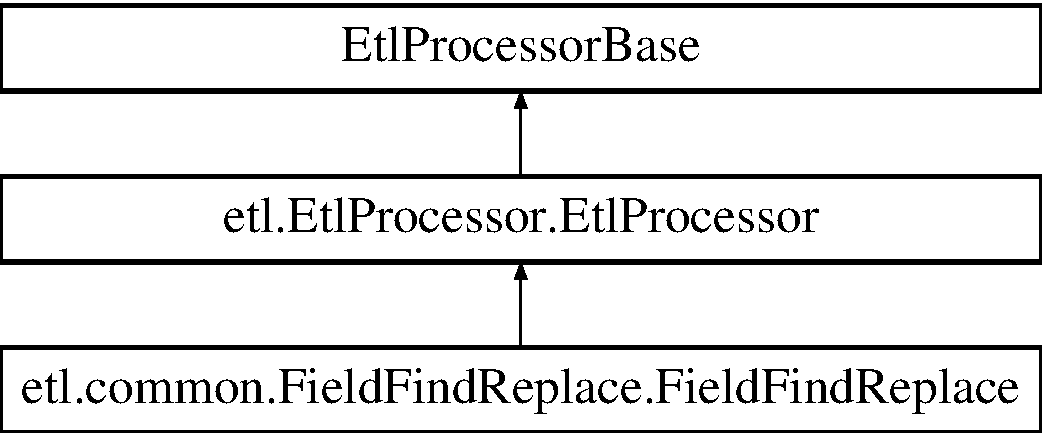
\includegraphics[height=3.000000cm]{classetl_1_1common_1_1FieldFindReplace_1_1FieldFindReplace}
\end{center}
\end{figure}
\subsection*{Public Member Functions}
\begin{DoxyCompactItemize}
\item 
def \hyperlink{classetl_1_1common_1_1FieldFindReplace_1_1FieldFindReplace_a06f3be0d398ee60bb5093e4d7b0ddc3e}{\-\_\-\-\_\-init\-\_\-\-\_\-}
\item 
\hypertarget{classetl_1_1common_1_1FieldFindReplace_1_1FieldFindReplace_a62b2e0343c81a6f1bd90ac8c8bdf3960}{def {\bfseries list\-\_\-inputs}}\label{classetl_1_1common_1_1FieldFindReplace_1_1FieldFindReplace_a62b2e0343c81a6f1bd90ac8c8bdf3960}

\item 
\hypertarget{classetl_1_1common_1_1FieldFindReplace_1_1FieldFindReplace_a75c72247a400b1a334c299528a6a516a}{def {\bfseries list\-\_\-outputs}}\label{classetl_1_1common_1_1FieldFindReplace_1_1FieldFindReplace_a75c72247a400b1a334c299528a6a516a}

\item 
\hypertarget{classetl_1_1common_1_1FieldFindReplace_1_1FieldFindReplace_aa9906be4a043348c4f9927ab36b40d51}{def {\bfseries replace}}\label{classetl_1_1common_1_1FieldFindReplace_1_1FieldFindReplace_aa9906be4a043348c4f9927ab36b40d51}

\item 
\hypertarget{classetl_1_1common_1_1FieldFindReplace_1_1FieldFindReplace_a50191dec5b9fdfa441437d7d3bc37f4b}{def {\bfseries regexp\-\_\-replace}}\label{classetl_1_1common_1_1FieldFindReplace_1_1FieldFindReplace_a50191dec5b9fdfa441437d7d3bc37f4b}

\end{DoxyCompactItemize}
\subsection*{Additional Inherited Members}


\subsection{Detailed Description}
\begin{DoxyVerb}Find and replace values in one or more fields

This processor performs a simple text search and replace on the input
records fields.  Call replace() ro regexp_replace() on processor to add
replacement rules.

This component uses the sames schema for output as is specified for the
input.
\end{DoxyVerb}
 

\subsection{Constructor \& Destructor Documentation}
\hypertarget{classetl_1_1common_1_1FieldFindReplace_1_1FieldFindReplace_a06f3be0d398ee60bb5093e4d7b0ddc3e}{\index{etl\-::common\-::\-Field\-Find\-Replace\-::\-Field\-Find\-Replace@{etl\-::common\-::\-Field\-Find\-Replace\-::\-Field\-Find\-Replace}!\-\_\-\-\_\-init\-\_\-\-\_\-@{\-\_\-\-\_\-init\-\_\-\-\_\-}}
\index{\-\_\-\-\_\-init\-\_\-\-\_\-@{\-\_\-\-\_\-init\-\_\-\-\_\-}!etl::common::FieldFindReplace::FieldFindReplace@{etl\-::common\-::\-Field\-Find\-Replace\-::\-Field\-Find\-Replace}}
\subsubsection[{\-\_\-\-\_\-init\-\_\-\-\_\-}]{\setlength{\rightskip}{0pt plus 5cm}def etl.\-common.\-Field\-Find\-Replace.\-Field\-Find\-Replace.\-\_\-\-\_\-init\-\_\-\-\_\- (
\begin{DoxyParamCaption}
\item[{}]{self, }
\item[{}]{schema, }
\item[{}]{input\-\_\-name = {\ttfamily 'records'}, }
\item[{}]{output\-\_\-name = {\ttfamily 'records'}}
\end{DoxyParamCaption}
)}}\label{classetl_1_1common_1_1FieldFindReplace_1_1FieldFindReplace_a06f3be0d398ee60bb5093e4d7b0ddc3e}
\begin{DoxyVerb}Init

@param schema: Schema to use for input and output records
@param input_name: Name of the processor input for connections
@param output_name: Name of the processor output for connections
\end{DoxyVerb}
 

The documentation for this class was generated from the following file\-:\begin{DoxyCompactItemize}
\item 
src/etl/common/Field\-Find\-Replace.\-py\end{DoxyCompactItemize}

\hypertarget{classetl_1_1EtlEvent_1_1EtlEvent}{\section{etl.\-Etl\-Event.\-Etl\-Event Class Reference}
\label{classetl_1_1EtlEvent_1_1EtlEvent}\index{etl.\-Etl\-Event.\-Etl\-Event@{etl.\-Etl\-Event.\-Etl\-Event}}
}
Inheritance diagram for etl.\-Etl\-Event.\-Etl\-Event\-:\begin{figure}[H]
\begin{center}
\leavevmode
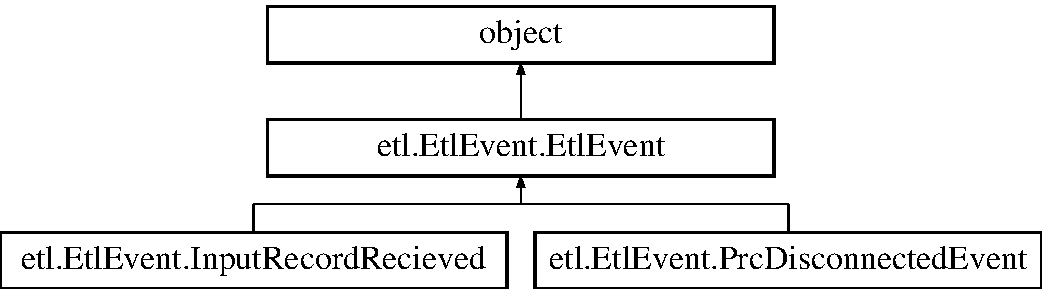
\includegraphics[height=3.000000cm]{classetl_1_1EtlEvent_1_1EtlEvent}
\end{center}
\end{figure}
\subsection*{Public Member Functions}
\begin{DoxyCompactItemize}
\item 
\hypertarget{classetl_1_1EtlEvent_1_1EtlEvent_a24f35282adb8d1d2d8b25a6bb06df3e8}{def {\bfseries \-\_\-\-\_\-init\-\_\-\-\_\-}}\label{classetl_1_1EtlEvent_1_1EtlEvent_a24f35282adb8d1d2d8b25a6bb06df3e8}

\item 
\hypertarget{classetl_1_1EtlEvent_1_1EtlEvent_a396c56109a4dc37ba40127a5dd1e5265}{def {\bfseries type}}\label{classetl_1_1EtlEvent_1_1EtlEvent_a396c56109a4dc37ba40127a5dd1e5265}

\end{DoxyCompactItemize}


\subsection{Detailed Description}
\begin{DoxyVerb}Notify an EtlProcessor of an event\end{DoxyVerb}
 

The documentation for this class was generated from the following file\-:\begin{DoxyCompactItemize}
\item 
src/etl/Etl\-Event.\-py\end{DoxyCompactItemize}

\hypertarget{classetl_1_1EtlEvent_1_1InputRecordRecieved}{\section{etl.\-Etl\-Event.\-Input\-Record\-Recieved Class Reference}
\label{classetl_1_1EtlEvent_1_1InputRecordRecieved}\index{etl.\-Etl\-Event.\-Input\-Record\-Recieved@{etl.\-Etl\-Event.\-Input\-Record\-Recieved}}
}
Inheritance diagram for etl.\-Etl\-Event.\-Input\-Record\-Recieved\-:\begin{figure}[H]
\begin{center}
\leavevmode
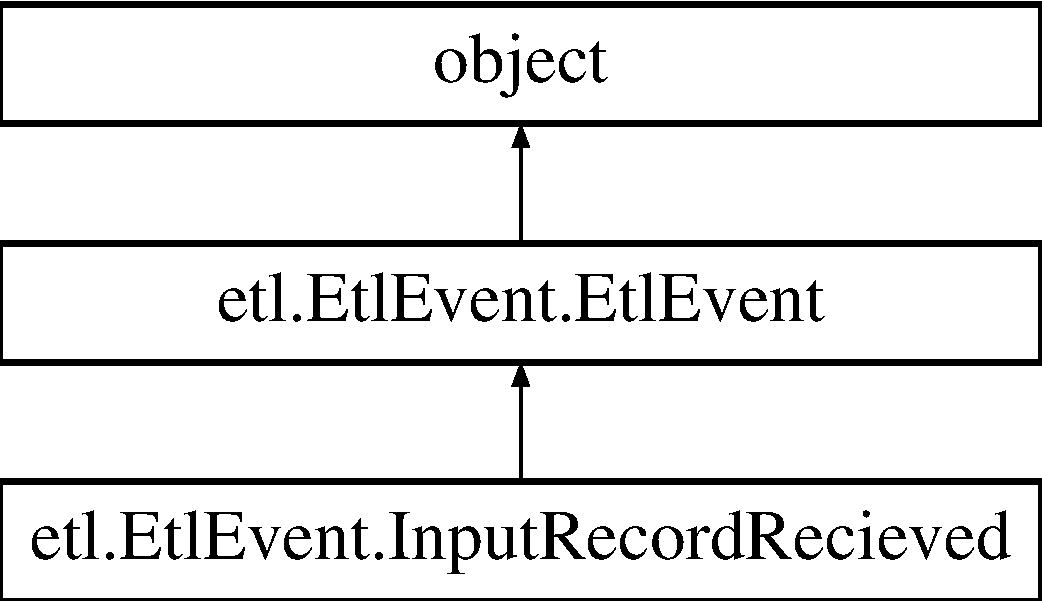
\includegraphics[height=3.000000cm]{classetl_1_1EtlEvent_1_1InputRecordRecieved}
\end{center}
\end{figure}
\subsection*{Public Member Functions}
\begin{DoxyCompactItemize}
\item 
\hypertarget{classetl_1_1EtlEvent_1_1InputRecordRecieved_a7282b013ccddb10fe1112b9e4aac7cdd}{def {\bfseries \-\_\-\-\_\-init\-\_\-\-\_\-}}\label{classetl_1_1EtlEvent_1_1InputRecordRecieved_a7282b013ccddb10fe1112b9e4aac7cdd}

\end{DoxyCompactItemize}
\subsection*{Public Attributes}
\begin{DoxyCompactItemize}
\item 
\hypertarget{classetl_1_1EtlEvent_1_1InputRecordRecieved_a5fc64da491760496be540ed6a2cda5c9}{{\bfseries input\-\_\-name}}\label{classetl_1_1EtlEvent_1_1InputRecordRecieved_a5fc64da491760496be540ed6a2cda5c9}

\item 
\hypertarget{classetl_1_1EtlEvent_1_1InputRecordRecieved_af8fccb01a2e7f48b56ffe9a100ac5f64}{{\bfseries conn\-\_\-id}}\label{classetl_1_1EtlEvent_1_1InputRecordRecieved_af8fccb01a2e7f48b56ffe9a100ac5f64}

\end{DoxyCompactItemize}


\subsection{Detailed Description}
\begin{DoxyVerb}An input record was received\end{DoxyVerb}
 

The documentation for this class was generated from the following file\-:\begin{DoxyCompactItemize}
\item 
src/etl/Etl\-Event.\-py\end{DoxyCompactItemize}

\hypertarget{classetl_1_1EtlEvent_1_1PrcDisconnectedEvent}{\section{etl.\-Etl\-Event.\-Prc\-Disconnected\-Event Class Reference}
\label{classetl_1_1EtlEvent_1_1PrcDisconnectedEvent}\index{etl.\-Etl\-Event.\-Prc\-Disconnected\-Event@{etl.\-Etl\-Event.\-Prc\-Disconnected\-Event}}
}
Inheritance diagram for etl.\-Etl\-Event.\-Prc\-Disconnected\-Event\-:\begin{figure}[H]
\begin{center}
\leavevmode
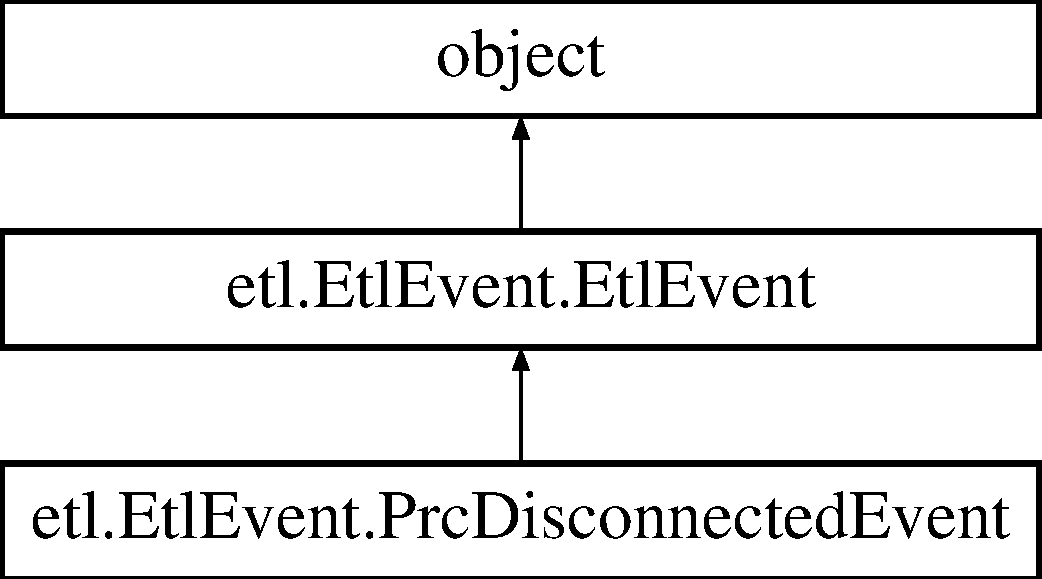
\includegraphics[height=3.000000cm]{classetl_1_1EtlEvent_1_1PrcDisconnectedEvent}
\end{center}
\end{figure}
\subsection*{Public Member Functions}
\begin{DoxyCompactItemize}
\item 
\hypertarget{classetl_1_1EtlEvent_1_1PrcDisconnectedEvent_ace6515dd505e4c88c29f52c7ca6ca37b}{def {\bfseries \-\_\-\-\_\-init\-\_\-\-\_\-}}\label{classetl_1_1EtlEvent_1_1PrcDisconnectedEvent_ace6515dd505e4c88c29f52c7ca6ca37b}

\end{DoxyCompactItemize}
\subsection*{Public Attributes}
\begin{DoxyCompactItemize}
\item 
\hypertarget{classetl_1_1EtlEvent_1_1PrcDisconnectedEvent_aba70f0d0a8c597bf251871d3b4f0e403}{{\bfseries input\-\_\-name}}\label{classetl_1_1EtlEvent_1_1PrcDisconnectedEvent_aba70f0d0a8c597bf251871d3b4f0e403}

\item 
\hypertarget{classetl_1_1EtlEvent_1_1PrcDisconnectedEvent_a4fad07f5bd96833a00455cfc3b699c9b}{{\bfseries src\-\_\-prc\-\_\-name}}\label{classetl_1_1EtlEvent_1_1PrcDisconnectedEvent_a4fad07f5bd96833a00455cfc3b699c9b}

\item 
\hypertarget{classetl_1_1EtlEvent_1_1PrcDisconnectedEvent_ac48e1e52a9419767be6e8e6958e870ad}{{\bfseries src\-\_\-output\-\_\-name}}\label{classetl_1_1EtlEvent_1_1PrcDisconnectedEvent_ac48e1e52a9419767be6e8e6958e870ad}

\item 
\hypertarget{classetl_1_1EtlEvent_1_1PrcDisconnectedEvent_a6a416398001426bff5d90e9c6d5ae451}{{\bfseries conn\-\_\-id}}\label{classetl_1_1EtlEvent_1_1PrcDisconnectedEvent_a6a416398001426bff5d90e9c6d5ae451}

\end{DoxyCompactItemize}


\subsection{Detailed Description}
\begin{DoxyVerb}A processor that a supplying processor has disconnected from it's input\end{DoxyVerb}
 

The documentation for this class was generated from the following file\-:\begin{DoxyCompactItemize}
\item 
src/etl/Etl\-Event.\-py\end{DoxyCompactItemize}

\hypertarget{classetl_1_1EtlJoinProcessor_1_1EtlJoinProcessor}{\section{etl.\-Etl\-Join\-Processor.\-Etl\-Join\-Processor Class Reference}
\label{classetl_1_1EtlJoinProcessor_1_1EtlJoinProcessor}\index{etl.\-Etl\-Join\-Processor.\-Etl\-Join\-Processor@{etl.\-Etl\-Join\-Processor.\-Etl\-Join\-Processor}}
}
Inheritance diagram for etl.\-Etl\-Join\-Processor.\-Etl\-Join\-Processor\-:\begin{figure}[H]
\begin{center}
\leavevmode
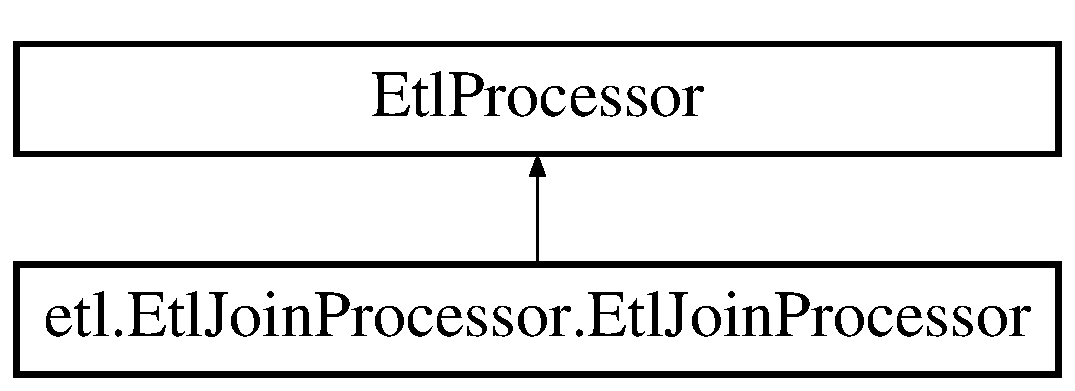
\includegraphics[height=2.000000cm]{classetl_1_1EtlJoinProcessor_1_1EtlJoinProcessor}
\end{center}
\end{figure}
\subsection*{Public Member Functions}
\begin{DoxyCompactItemize}
\item 
\hypertarget{classetl_1_1EtlJoinProcessor_1_1EtlJoinProcessor_a88ffde25fdd2cc96ee2f1528cd019f4d}{def {\bfseries \-\_\-\-\_\-init\-\_\-\-\_\-}}\label{classetl_1_1EtlJoinProcessor_1_1EtlJoinProcessor_a88ffde25fdd2cc96ee2f1528cd019f4d}

\item 
\hypertarget{classetl_1_1EtlJoinProcessor_1_1EtlJoinProcessor_a3b4bfc44895abfb740ae6c3ea93b2306}{def {\bfseries list\-\_\-inputs}}\label{classetl_1_1EtlJoinProcessor_1_1EtlJoinProcessor_a3b4bfc44895abfb740ae6c3ea93b2306}

\item 
def \hyperlink{classetl_1_1EtlJoinProcessor_1_1EtlJoinProcessor_ab19040ec6313ce7cf54e1f2dc9d834de}{list\-\_\-lookup\-\_\-inputs}
\item 
def \hyperlink{classetl_1_1EtlJoinProcessor_1_1EtlJoinProcessor_a3dc84a5aa91be7bc9323edbea0a5e121}{list\-\_\-subject\-\_\-inputs}
\item 
def \hyperlink{classetl_1_1EtlJoinProcessor_1_1EtlJoinProcessor_a06eafbd5af31068c07ed050327396708}{build\-\_\-lookup\-\_\-record\-\_\-key}
\item 
def \hyperlink{classetl_1_1EtlJoinProcessor_1_1EtlJoinProcessor_a39409cd0d1a82d79ad238832500bf543}{build\-\_\-lookup\-\_\-key}
\item 
def \hyperlink{classetl_1_1EtlJoinProcessor_1_1EtlJoinProcessor_aed55617ed6415c98f3cb12b5af04bf74}{gen\-\_\-output}
\item 
def \hyperlink{classetl_1_1EtlJoinProcessor_1_1EtlJoinProcessor_a61b0670d226d114b033548b87d4d3f11}{lookup}
\end{DoxyCompactItemize}


\subsection{Detailed Description}
\begin{DoxyVerb}Join one set of records to another\end{DoxyVerb}
 

\subsection{Member Function Documentation}
\hypertarget{classetl_1_1EtlJoinProcessor_1_1EtlJoinProcessor_a39409cd0d1a82d79ad238832500bf543}{\index{etl\-::\-Etl\-Join\-Processor\-::\-Etl\-Join\-Processor@{etl\-::\-Etl\-Join\-Processor\-::\-Etl\-Join\-Processor}!build\-\_\-lookup\-\_\-key@{build\-\_\-lookup\-\_\-key}}
\index{build\-\_\-lookup\-\_\-key@{build\-\_\-lookup\-\_\-key}!etl::EtlJoinProcessor::EtlJoinProcessor@{etl\-::\-Etl\-Join\-Processor\-::\-Etl\-Join\-Processor}}
\subsubsection[{build\-\_\-lookup\-\_\-key}]{\setlength{\rightskip}{0pt plus 5cm}def etl.\-Etl\-Join\-Processor.\-Etl\-Join\-Processor.\-build\-\_\-lookup\-\_\-key (
\begin{DoxyParamCaption}
\item[{}]{self, }
\item[{}]{record}
\end{DoxyParamCaption}
)}}\label{classetl_1_1EtlJoinProcessor_1_1EtlJoinProcessor_a39409cd0d1a82d79ad238832500bf543}
\begin{DoxyVerb}Build a key to use to find a lookup record\end{DoxyVerb}
 \hypertarget{classetl_1_1EtlJoinProcessor_1_1EtlJoinProcessor_a06eafbd5af31068c07ed050327396708}{\index{etl\-::\-Etl\-Join\-Processor\-::\-Etl\-Join\-Processor@{etl\-::\-Etl\-Join\-Processor\-::\-Etl\-Join\-Processor}!build\-\_\-lookup\-\_\-record\-\_\-key@{build\-\_\-lookup\-\_\-record\-\_\-key}}
\index{build\-\_\-lookup\-\_\-record\-\_\-key@{build\-\_\-lookup\-\_\-record\-\_\-key}!etl::EtlJoinProcessor::EtlJoinProcessor@{etl\-::\-Etl\-Join\-Processor\-::\-Etl\-Join\-Processor}}
\subsubsection[{build\-\_\-lookup\-\_\-record\-\_\-key}]{\setlength{\rightskip}{0pt plus 5cm}def etl.\-Etl\-Join\-Processor.\-Etl\-Join\-Processor.\-build\-\_\-lookup\-\_\-record\-\_\-key (
\begin{DoxyParamCaption}
\item[{}]{self, }
\item[{}]{lookup\-\_\-record}
\end{DoxyParamCaption}
)}}\label{classetl_1_1EtlJoinProcessor_1_1EtlJoinProcessor_a06eafbd5af31068c07ed050327396708}
\begin{DoxyVerb}Build a key to be used for matching subject records to\end{DoxyVerb}
 \hypertarget{classetl_1_1EtlJoinProcessor_1_1EtlJoinProcessor_aed55617ed6415c98f3cb12b5af04bf74}{\index{etl\-::\-Etl\-Join\-Processor\-::\-Etl\-Join\-Processor@{etl\-::\-Etl\-Join\-Processor\-::\-Etl\-Join\-Processor}!gen\-\_\-output@{gen\-\_\-output}}
\index{gen\-\_\-output@{gen\-\_\-output}!etl::EtlJoinProcessor::EtlJoinProcessor@{etl\-::\-Etl\-Join\-Processor\-::\-Etl\-Join\-Processor}}
\subsubsection[{gen\-\_\-output}]{\setlength{\rightskip}{0pt plus 5cm}def etl.\-Etl\-Join\-Processor.\-Etl\-Join\-Processor.\-gen\-\_\-output (
\begin{DoxyParamCaption}
\item[{}]{self, }
\item[{}]{name, }
\item[{}]{inputs, }
\item[{}]{record\-\_\-set}
\end{DoxyParamCaption}
)}}\label{classetl_1_1EtlJoinProcessor_1_1EtlJoinProcessor_aed55617ed6415c98f3cb12b5af04bf74}
\begin{DoxyVerb}Generate named output data.

Dynamically calls 'gen_<name>_output' method

@param name: Name of the output to generate
@param inputs: Dictionary of connected input datasets
@param record_set: Container to populate with records
\end{DoxyVerb}
 \hypertarget{classetl_1_1EtlJoinProcessor_1_1EtlJoinProcessor_ab19040ec6313ce7cf54e1f2dc9d834de}{\index{etl\-::\-Etl\-Join\-Processor\-::\-Etl\-Join\-Processor@{etl\-::\-Etl\-Join\-Processor\-::\-Etl\-Join\-Processor}!list\-\_\-lookup\-\_\-inputs@{list\-\_\-lookup\-\_\-inputs}}
\index{list\-\_\-lookup\-\_\-inputs@{list\-\_\-lookup\-\_\-inputs}!etl::EtlJoinProcessor::EtlJoinProcessor@{etl\-::\-Etl\-Join\-Processor\-::\-Etl\-Join\-Processor}}
\subsubsection[{list\-\_\-lookup\-\_\-inputs}]{\setlength{\rightskip}{0pt plus 5cm}def etl.\-Etl\-Join\-Processor.\-Etl\-Join\-Processor.\-list\-\_\-lookup\-\_\-inputs (
\begin{DoxyParamCaption}
\item[{}]{self}
\end{DoxyParamCaption}
)}}\label{classetl_1_1EtlJoinProcessor_1_1EtlJoinProcessor_ab19040ec6313ce7cf54e1f2dc9d834de}
\begin{DoxyVerb}List inputs that contain the records to ref against

These record sets must be indexed
\end{DoxyVerb}
 \hypertarget{classetl_1_1EtlJoinProcessor_1_1EtlJoinProcessor_a3dc84a5aa91be7bc9323edbea0a5e121}{\index{etl\-::\-Etl\-Join\-Processor\-::\-Etl\-Join\-Processor@{etl\-::\-Etl\-Join\-Processor\-::\-Etl\-Join\-Processor}!list\-\_\-subject\-\_\-inputs@{list\-\_\-subject\-\_\-inputs}}
\index{list\-\_\-subject\-\_\-inputs@{list\-\_\-subject\-\_\-inputs}!etl::EtlJoinProcessor::EtlJoinProcessor@{etl\-::\-Etl\-Join\-Processor\-::\-Etl\-Join\-Processor}}
\subsubsection[{list\-\_\-subject\-\_\-inputs}]{\setlength{\rightskip}{0pt plus 5cm}def etl.\-Etl\-Join\-Processor.\-Etl\-Join\-Processor.\-list\-\_\-subject\-\_\-inputs (
\begin{DoxyParamCaption}
\item[{}]{self}
\end{DoxyParamCaption}
)}}\label{classetl_1_1EtlJoinProcessor_1_1EtlJoinProcessor_a3dc84a5aa91be7bc9323edbea0a5e121}
\begin{DoxyVerb}List inputs that contain the records to find refs for\end{DoxyVerb}
 \hypertarget{classetl_1_1EtlJoinProcessor_1_1EtlJoinProcessor_a61b0670d226d114b033548b87d4d3f11}{\index{etl\-::\-Etl\-Join\-Processor\-::\-Etl\-Join\-Processor@{etl\-::\-Etl\-Join\-Processor\-::\-Etl\-Join\-Processor}!lookup@{lookup}}
\index{lookup@{lookup}!etl::EtlJoinProcessor::EtlJoinProcessor@{etl\-::\-Etl\-Join\-Processor\-::\-Etl\-Join\-Processor}}
\subsubsection[{lookup}]{\setlength{\rightskip}{0pt plus 5cm}def etl.\-Etl\-Join\-Processor.\-Etl\-Join\-Processor.\-lookup (
\begin{DoxyParamCaption}
\item[{}]{self, }
\item[{}]{record}
\end{DoxyParamCaption}
)}}\label{classetl_1_1EtlJoinProcessor_1_1EtlJoinProcessor_a61b0670d226d114b033548b87d4d3f11}
\begin{DoxyVerb}Find record in lookup sets for this record\end{DoxyVerb}
 

The documentation for this class was generated from the following file\-:\begin{DoxyCompactItemize}
\item 
src/etl/Etl\-Join\-Processor.\-py\end{DoxyCompactItemize}

\hypertarget{classetl_1_1EtlProcessor_1_1EtlProcessor}{\section{etl.\-Etl\-Processor.\-Etl\-Processor Class Reference}
\label{classetl_1_1EtlProcessor_1_1EtlProcessor}\index{etl.\-Etl\-Processor.\-Etl\-Processor@{etl.\-Etl\-Processor.\-Etl\-Processor}}
}
Inheritance diagram for etl.\-Etl\-Processor.\-Etl\-Processor\-:\begin{figure}[H]
\begin{center}
\leavevmode
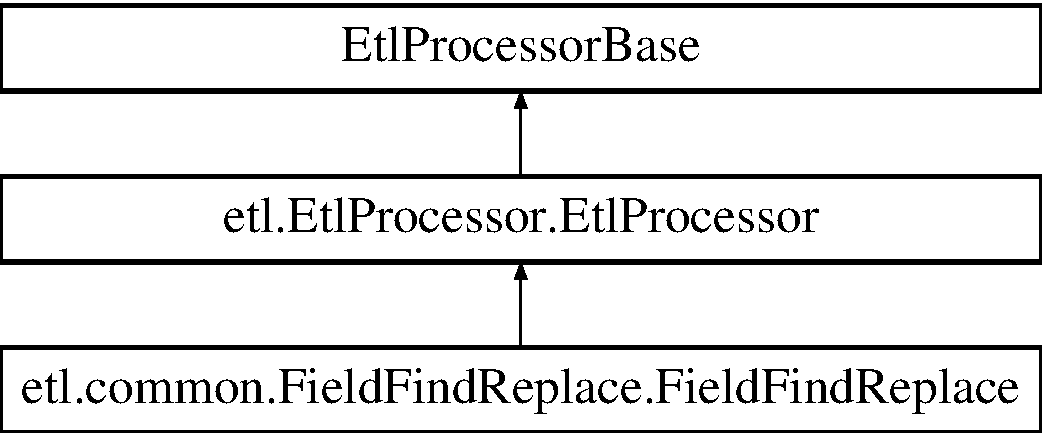
\includegraphics[height=3.000000cm]{classetl_1_1EtlProcessor_1_1EtlProcessor}
\end{center}
\end{figure}
\subsection*{Public Member Functions}
\begin{DoxyCompactItemize}
\item 
\hypertarget{classetl_1_1EtlProcessor_1_1EtlProcessor_a2f31216d32806e4b4495399da7d0c024}{def {\bfseries \-\_\-\-\_\-init\-\_\-\-\_\-}}\label{classetl_1_1EtlProcessor_1_1EtlProcessor_a2f31216d32806e4b4495399da7d0c024}

\item 
def \hyperlink{classetl_1_1EtlProcessor_1_1EtlProcessor_acda16c0d22a7b2d80de6d62133acce0d}{extract\-\_\-records}
\end{DoxyCompactItemize}
\subsection*{Public Attributes}
\begin{DoxyCompactItemize}
\item 
\hypertarget{classetl_1_1EtlProcessor_1_1EtlProcessor_afff0c61d3a059fa201bc0da59a269651}{{\bfseries data\-\_\-dir\-\_\-path}}\label{classetl_1_1EtlProcessor_1_1EtlProcessor_afff0c61d3a059fa201bc0da59a269651}

\item 
\hypertarget{classetl_1_1EtlProcessor_1_1EtlProcessor_aa0175c614fa82691f7177b2e7bd44c4a}{{\bfseries tmp\-\_\-dir\-\_\-path}}\label{classetl_1_1EtlProcessor_1_1EtlProcessor_aa0175c614fa82691f7177b2e7bd44c4a}

\end{DoxyCompactItemize}


\subsection{Detailed Description}
\begin{DoxyVerb}Takes 0 or more inputs and generates 0 or more outputs

See EtlProcessorBase for additional detail

The EtlProcessor class is intended to be subclassed in order to create 
the components of the ETL processor.  Each processor, then, performs one or
more of the Extract, Transform, or Load functions in it's own thread.

When subclassing, you must:

1)  In your __init__():
    a) Call the super init()
    b) Call df_create_input_port() to define input ports
    c) Call df_create_output_port() to define output ports

2)  (optionally) define starting_processor() to perform any startup tasks

3)  (optionally) define extract_records() to extract records from external
     sources and output them for use by other processors

       - Call dispatch_output() to send generated records out

4)  (optionally) define methods to process records sent to this component's 
    input ports.

      - Define pr_<name>_input_record() to process records recieved on
        port named <name>.
      - Define pr_any_input_record() to consume incoming records not handled
        by a method setup for a speific port name.

      - Call pr_dispatch_output() to send processed records out
      - Call pr_hold_record() to stash a record for processing later
      - Call pr_unhold_records() to retrieve previously held records
      - Call pr_output_finished() to signal that no more output will
        be sent on the named port.  When all output ports are clossed,
        then the processing loop will exit.

5)  Define pr_handle_input_clossed() to perform any final processing when
    an input port is clossed.  All of the methods available to the input
    handling methods are available here.
\end{DoxyVerb}
 

\subsection{Member Function Documentation}
\hypertarget{classetl_1_1EtlProcessor_1_1EtlProcessor_acda16c0d22a7b2d80de6d62133acce0d}{\index{etl\-::\-Etl\-Processor\-::\-Etl\-Processor@{etl\-::\-Etl\-Processor\-::\-Etl\-Processor}!extract\-\_\-records@{extract\-\_\-records}}
\index{extract\-\_\-records@{extract\-\_\-records}!etl::EtlProcessor::EtlProcessor@{etl\-::\-Etl\-Processor\-::\-Etl\-Processor}}
\subsubsection[{extract\-\_\-records}]{\setlength{\rightskip}{0pt plus 5cm}def etl.\-Etl\-Processor.\-Etl\-Processor.\-extract\-\_\-records (
\begin{DoxyParamCaption}
\item[{}]{self}
\end{DoxyParamCaption}
)}}\label{classetl_1_1EtlProcessor_1_1EtlProcessor_acda16c0d22a7b2d80de6d62133acce0d}
\begin{DoxyVerb}Hook for processor to extract/generate records

These are records that are *not* created from processing input records,
but rather are generated completely by the processor.  It is called
before any input records are received if inputs are connected.

If you need to generate records after all input records are processed,
use the handle_input_disconnected() hook.
\end{DoxyVerb}
 

The documentation for this class was generated from the following file\-:\begin{DoxyCompactItemize}
\item 
src/etl/Etl\-Processor.\-py\end{DoxyCompactItemize}

\hypertarget{classetl_1_1EtlProcessor_1_1EtlProcessorDataPort}{\section{etl.\-Etl\-Processor.\-Etl\-Processor\-Data\-Port Class Reference}
\label{classetl_1_1EtlProcessor_1_1EtlProcessorDataPort}\index{etl.\-Etl\-Processor.\-Etl\-Processor\-Data\-Port@{etl.\-Etl\-Processor.\-Etl\-Processor\-Data\-Port}}
}
Inheritance diagram for etl.\-Etl\-Processor.\-Etl\-Processor\-Data\-Port\-:\begin{figure}[H]
\begin{center}
\leavevmode
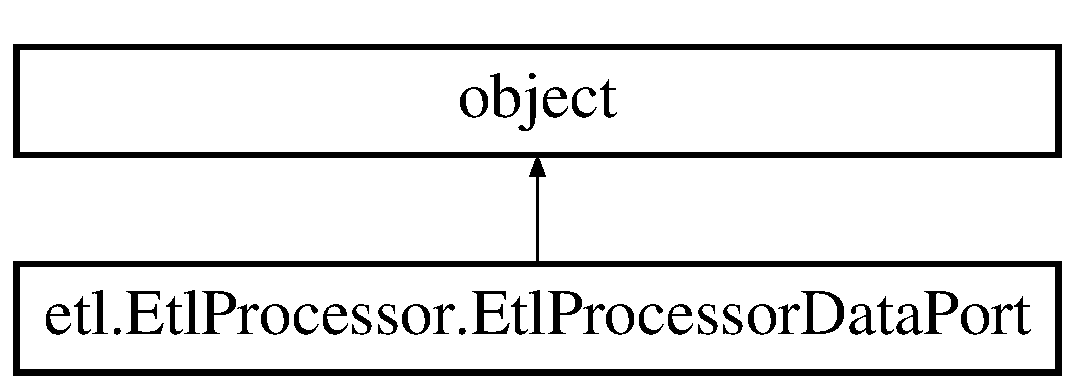
\includegraphics[height=2.000000cm]{classetl_1_1EtlProcessor_1_1EtlProcessorDataPort}
\end{center}
\end{figure}
\subsection*{Public Member Functions}
\begin{DoxyCompactItemize}
\item 
\hypertarget{classetl_1_1EtlProcessor_1_1EtlProcessorDataPort_a5af394c5e2bd3873b965c89ad367a7d3}{def {\bfseries \-\_\-\-\_\-init\-\_\-\-\_\-}}\label{classetl_1_1EtlProcessor_1_1EtlProcessorDataPort_a5af394c5e2bd3873b965c89ad367a7d3}

\end{DoxyCompactItemize}
\subsection*{Public Attributes}
\begin{DoxyCompactItemize}
\item 
\hypertarget{classetl_1_1EtlProcessor_1_1EtlProcessorDataPort_a8826839584c592bd39e0d5dd5fed939d}{{\bfseries name}}\label{classetl_1_1EtlProcessor_1_1EtlProcessorDataPort_a8826839584c592bd39e0d5dd5fed939d}

\item 
\hypertarget{classetl_1_1EtlProcessor_1_1EtlProcessorDataPort_a9c951d12496f5094604451f8a445f956}{{\bfseries schema}}\label{classetl_1_1EtlProcessor_1_1EtlProcessorDataPort_a9c951d12496f5094604451f8a445f956}

\end{DoxyCompactItemize}


\subsection{Detailed Description}
\begin{DoxyVerb}Specify a name for input or output record sets\end{DoxyVerb}
 

The documentation for this class was generated from the following file\-:\begin{DoxyCompactItemize}
\item 
src/etl/Etl\-Processor.\-py\end{DoxyCompactItemize}

\hypertarget{classetl_1_1EtlProcessorBase_1_1EtlProcessorBase}{\section{etl.\-Etl\-Processor\-Base.\-Etl\-Processor\-Base Class Reference}
\label{classetl_1_1EtlProcessorBase_1_1EtlProcessorBase}\index{etl.\-Etl\-Processor\-Base.\-Etl\-Processor\-Base@{etl.\-Etl\-Processor\-Base.\-Etl\-Processor\-Base}}
}
Inheritance diagram for etl.\-Etl\-Processor\-Base.\-Etl\-Processor\-Base\-:\begin{figure}[H]
\begin{center}
\leavevmode
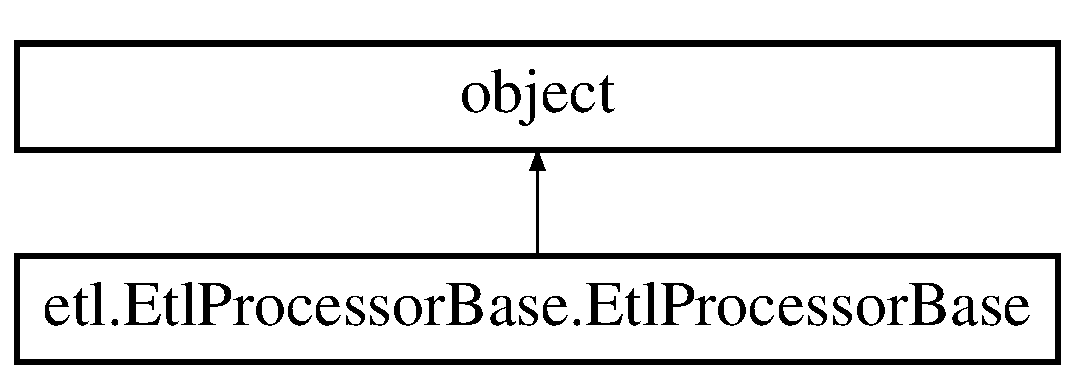
\includegraphics[height=2.000000cm]{classetl_1_1EtlProcessorBase_1_1EtlProcessorBase}
\end{center}
\end{figure}
\subsection*{Public Member Functions}
\begin{DoxyCompactItemize}
\item 
\hypertarget{classetl_1_1EtlProcessorBase_1_1EtlProcessorBase_a5f5cbe4f638a7960a9d2acb9d8d41c4d}{def {\bfseries \-\_\-\-\_\-init\-\_\-\-\_\-}}\label{classetl_1_1EtlProcessorBase_1_1EtlProcessorBase_a5f5cbe4f638a7960a9d2acb9d8d41c4d}

\item 
def \hyperlink{classetl_1_1EtlProcessorBase_1_1EtlProcessorBase_ae0946b935a1d48c58791d3093401dc3b}{current\-\_\-state}
\item 
def \hyperlink{classetl_1_1EtlProcessorBase_1_1EtlProcessorBase_aae68b2482869b7ef16ba7060eb697f0a}{current\-\_\-state\-\_\-desc}
\item 
def \hyperlink{classetl_1_1EtlProcessorBase_1_1EtlProcessorBase_a9f07bf2c83f0d88aa18e6cf14307c1d7}{df\-\_\-create\-\_\-input\-\_\-port}
\item 
def \hyperlink{classetl_1_1EtlProcessorBase_1_1EtlProcessorBase_aa381c6d1c2a46d944bf6e38f35c1bd09}{df\-\_\-create\-\_\-output\-\_\-port}
\item 
def \hyperlink{classetl_1_1EtlProcessorBase_1_1EtlProcessorBase_a9c6d70b1b3cc1a4e4e16f99c66ef16f5}{start\-\_\-processor}
\item 
def \hyperlink{classetl_1_1EtlProcessorBase_1_1EtlProcessorBase_af76118658743124b1ec374c8b9efb3ef}{waiting\-\_\-on\-\_\-more\-\_\-input}
\item 
def \hyperlink{classetl_1_1EtlProcessorBase_1_1EtlProcessorBase_aa1514472c9ed48feae21629a7afa19b4}{dispatch\-\_\-output\-\_\-record}
\item 
def \hyperlink{classetl_1_1EtlProcessorBase_1_1EtlProcessorBase_a016207be9c5cfa047a3e50355fa1d7f3}{notify\-\_\-dispatch\-\_\-error}
\item 
def \hyperlink{classetl_1_1EtlProcessorBase_1_1EtlProcessorBase_ac63c59ee7858b2d7f8d8c57a82469e39}{notify\-\_\-record\-\_\-error}
\item 
\hypertarget{classetl_1_1EtlProcessorBase_1_1EtlProcessorBase_a232eb2642f9da1d49ebe7aaf8bc244c5}{def {\bfseries notify\-\_\-error}}\label{classetl_1_1EtlProcessorBase_1_1EtlProcessorBase_a232eb2642f9da1d49ebe7aaf8bc244c5}

\item 
\hypertarget{classetl_1_1EtlProcessorBase_1_1EtlProcessorBase_ae7bc56cdbd7fb9d02259ba34602378f2}{def {\bfseries get\-\_\-event\-\_\-queue}}\label{classetl_1_1EtlProcessorBase_1_1EtlProcessorBase_ae7bc56cdbd7fb9d02259ba34602378f2}

\item 
\hypertarget{classetl_1_1EtlProcessorBase_1_1EtlProcessorBase_ab9341af5f174eecff55b1ac1be7c8246}{def {\bfseries get\-\_\-record\-\_\-queue}}\label{classetl_1_1EtlProcessorBase_1_1EtlProcessorBase_ab9341af5f174eecff55b1ac1be7c8246}

\item 
def \hyperlink{classetl_1_1EtlProcessorBase_1_1EtlProcessorBase_ad9b0b04dcac7b59d8cbe00c3f36a0ce9}{df\-\_\-add\-\_\-child\-\_\-processor}
\end{DoxyCompactItemize}
\subsection*{Public Attributes}
\begin{DoxyCompactItemize}
\item 
\hypertarget{classetl_1_1EtlProcessorBase_1_1EtlProcessorBase_a734c7d87d4efa8c235c216f7455f8044}{{\bfseries input\-\_\-queue}}\label{classetl_1_1EtlProcessorBase_1_1EtlProcessorBase_a734c7d87d4efa8c235c216f7455f8044}

\end{DoxyCompactItemize}
\subsection*{Static Public Attributes}
\begin{DoxyCompactItemize}
\item 
\hypertarget{classetl_1_1EtlProcessorBase_1_1EtlProcessorBase_ada4a767f0298a8036738f8be0a1e1c0f}{int {\bfseries S\-E\-T\-U\-P\-\_\-\-P\-H\-A\-S\-E} = 1}\label{classetl_1_1EtlProcessorBase_1_1EtlProcessorBase_ada4a767f0298a8036738f8be0a1e1c0f}

\item 
\hypertarget{classetl_1_1EtlProcessorBase_1_1EtlProcessorBase_a0d098520d6441ba28382092d79632ed1}{int {\bfseries S\-T\-A\-R\-T\-U\-P\-\_\-\-P\-H\-A\-S\-E} = 2}\label{classetl_1_1EtlProcessorBase_1_1EtlProcessorBase_a0d098520d6441ba28382092d79632ed1}

\item 
\hypertarget{classetl_1_1EtlProcessorBase_1_1EtlProcessorBase_abaa2ad4994bcc4214b9017900f1ff7f2}{int {\bfseries R\-U\-N\-N\-I\-N\-G\-\_\-\-P\-H\-A\-S\-E} = 3}\label{classetl_1_1EtlProcessorBase_1_1EtlProcessorBase_abaa2ad4994bcc4214b9017900f1ff7f2}

\item 
\hypertarget{classetl_1_1EtlProcessorBase_1_1EtlProcessorBase_a0439d55a6b6789992f3004fe377f0006}{int {\bfseries F\-I\-N\-I\-S\-H\-E\-D} = 4}\label{classetl_1_1EtlProcessorBase_1_1EtlProcessorBase_a0439d55a6b6789992f3004fe377f0006}

\item 
dictionary {\bfseries S\-T\-A\-T\-E\-\_\-\-D\-E\-S\-C}
\item 
\hypertarget{classetl_1_1EtlProcessorBase_1_1EtlProcessorBase_af8e5e9872734886bfef3db710f683885}{int {\bfseries M\-A\-X\-\_\-\-E\-V\-E\-N\-T\-\_\-\-Q\-\_\-\-S\-I\-Z\-E} = 1000}\label{classetl_1_1EtlProcessorBase_1_1EtlProcessorBase_af8e5e9872734886bfef3db710f683885}

\item 
\hypertarget{classetl_1_1EtlProcessorBase_1_1EtlProcessorBase_a40c5025f0561e5c67a98c9101ec7a9d8}{int {\bfseries M\-A\-X\-\_\-\-R\-E\-C\-O\-R\-D\-\_\-\-Q\-\_\-\-S\-Z\-I\-E} = 100}\label{classetl_1_1EtlProcessorBase_1_1EtlProcessorBase_a40c5025f0561e5c67a98c9101ec7a9d8}

\end{DoxyCompactItemize}


\subsection{Detailed Description}
\begin{DoxyVerb}Base class for EtlProcessor

Each Processor goes through these states.  The current state can be queried
by the current_state property.

SETUP_PHASE       - Is the phase before processor is started.  This is the
                    the processor starts in, and is meant to provide time to
                    configure the component prior to starting the ETL process.

STARTUP_PHASE     - Is the state that the processor enters while starting the
                    ETL process, before the processor starts reciving or
                    dispatching records.

PAUSED            - Temporary state to stop processing

RUNNING_PHASE     - Is the state that the processor is in while it is 
                    processing (recieving and dispatching) records.

FINSIHED_PHASE    - Is the status the the processor is in when it will no
                    longer recieve or dispatch records.


                +-------+   start_processor()   +---------+
                | SETUP +-----------------------> STARTUP |
                +-------+                       +----+----+
                                                     |     
                                               after |     
                                 starting_processor()|     
                                                call |     
                                                     |     
               +--------+   pause_processor()   +----v----+
               | PAUSED <-----------------------> RUNNING |
               +--------+  resume_processor()   +----+----+
                                                     |     
                                        after inputs |     
                                         and outputs |     
                                          all closed |     
                                                     |     
                                               +-----v----+
                                               | FINISHED |
                                               +----------+    


Because Processors have multiple stages, and run in threads, knowing
which method can be called when gets complex.  Here is the convention
used to keep information organized:

| Name  |       Desc          |   Called by       |
|-------|---------------------|-------------------|
| df_*  | Definition Methods  | Self during setup |
| st_*  | Static/Thread Safe  | Anyone            |
| if_*  | Interface           | Other Processors  |
| ct_*  | Control             | Parent Processor  |
| pr_*  | Processing          | Inside Prc Thread |

Each method may also check to verify that it is only called in specific
phases by calling one of the _*_phase_method() methods as the first line
of the method.  This serves both to remember when the method can be
called, and to enforce.


|       Method       | SETUP | STARTUP | RUNNING | FINISHED |
|--------------------|-------|---------|---------|----------|
| create_input_port  |   *   |         |         |          |
| create_output_port |   *   |         |         |          |
| _lock_input_port   |   *   |         |         |          |
| _unlock_input_port |       |   *     |         |          |


Interface methods interact with the internal thread safe queue to allow
external processors (or any external objects) to send signals/records to
this processor to work on.  Unlike previous versions of this ETL, external
objects do not push objects into the queue directly.  This is to help
keep the definition of the "Event" next to the handler for that event.
That is, you don't have an Event object, that needs to have the same
parameters as the handling method.  So, in general:

1) An external method calls an if_* method like if_receive_input()
   using that methods normal signature.

2) The interface method describes that call with an object and 
   queues it to the thread safe event_queue
   
3) pr_process_events() picks up that call description object from
   the queue and calls the pr_* version of the interface method,
   such as pr_receive_input().

    +----------------------------------------------------------+    
    |                                |                         |    
    |           if_<name>(args) +----------------> Queue       |    
    |                                |               +         |
    |                                |               |         |    
    | (outside thread)               |               |         |    
    |--------------------------------+               |         |    
    | (inside thread)                                |         |    
    |                                                v         |    
    |           pr_<name>(args) <------------+ pr_event_loop() |
    +----------------------------------------------------------+
            

Sub Processors
--------------

While typically, only the root processor will have children processors,
support is built into this base class for keeping track of children
processors.

The parent processor of a child processor is responsible for tracking
the status of all of it's children, and not considering itself finished
until all of the child processes are finished.

In general, connections can be formed between:

  - Two processes that are sblings of the same parent with the
    df_connect_sib_processors() method
  - From a parent output down to one of it's children's input
    ports with df_connect_parent_to_child()
  - From one of a parent processor's children's output up to a parent
    input port using df_connect_child_to_parent()

Child processors are added to this processor by calling
df_add_child_processor().  

@see EtlProcessor
\end{DoxyVerb}
 

\subsection{Member Function Documentation}
\hypertarget{classetl_1_1EtlProcessorBase_1_1EtlProcessorBase_ae0946b935a1d48c58791d3093401dc3b}{\index{etl\-::\-Etl\-Processor\-Base\-::\-Etl\-Processor\-Base@{etl\-::\-Etl\-Processor\-Base\-::\-Etl\-Processor\-Base}!current\-\_\-state@{current\-\_\-state}}
\index{current\-\_\-state@{current\-\_\-state}!etl::EtlProcessorBase::EtlProcessorBase@{etl\-::\-Etl\-Processor\-Base\-::\-Etl\-Processor\-Base}}
\subsubsection[{current\-\_\-state}]{\setlength{\rightskip}{0pt plus 5cm}def etl.\-Etl\-Processor\-Base.\-Etl\-Processor\-Base.\-current\-\_\-state (
\begin{DoxyParamCaption}
\item[{}]{self}
\end{DoxyParamCaption}
)}}\label{classetl_1_1EtlProcessorBase_1_1EtlProcessorBase_ae0946b935a1d48c58791d3093401dc3b}
\begin{DoxyVerb}Current state of this processor\end{DoxyVerb}
 \hypertarget{classetl_1_1EtlProcessorBase_1_1EtlProcessorBase_aae68b2482869b7ef16ba7060eb697f0a}{\index{etl\-::\-Etl\-Processor\-Base\-::\-Etl\-Processor\-Base@{etl\-::\-Etl\-Processor\-Base\-::\-Etl\-Processor\-Base}!current\-\_\-state\-\_\-desc@{current\-\_\-state\-\_\-desc}}
\index{current\-\_\-state\-\_\-desc@{current\-\_\-state\-\_\-desc}!etl::EtlProcessorBase::EtlProcessorBase@{etl\-::\-Etl\-Processor\-Base\-::\-Etl\-Processor\-Base}}
\subsubsection[{current\-\_\-state\-\_\-desc}]{\setlength{\rightskip}{0pt plus 5cm}def etl.\-Etl\-Processor\-Base.\-Etl\-Processor\-Base.\-current\-\_\-state\-\_\-desc (
\begin{DoxyParamCaption}
\item[{}]{self}
\end{DoxyParamCaption}
)}}\label{classetl_1_1EtlProcessorBase_1_1EtlProcessorBase_aae68b2482869b7ef16ba7060eb697f0a}
\begin{DoxyVerb}Friendly description of current state\end{DoxyVerb}
 \hypertarget{classetl_1_1EtlProcessorBase_1_1EtlProcessorBase_ad9b0b04dcac7b59d8cbe00c3f36a0ce9}{\index{etl\-::\-Etl\-Processor\-Base\-::\-Etl\-Processor\-Base@{etl\-::\-Etl\-Processor\-Base\-::\-Etl\-Processor\-Base}!df\-\_\-add\-\_\-child\-\_\-processor@{df\-\_\-add\-\_\-child\-\_\-processor}}
\index{df\-\_\-add\-\_\-child\-\_\-processor@{df\-\_\-add\-\_\-child\-\_\-processor}!etl::EtlProcessorBase::EtlProcessorBase@{etl\-::\-Etl\-Processor\-Base\-::\-Etl\-Processor\-Base}}
\subsubsection[{df\-\_\-add\-\_\-child\-\_\-processor}]{\setlength{\rightskip}{0pt plus 5cm}def etl.\-Etl\-Processor\-Base.\-Etl\-Processor\-Base.\-df\-\_\-add\-\_\-child\-\_\-processor (
\begin{DoxyParamCaption}
\item[{}]{self, }
\item[{}]{child}
\end{DoxyParamCaption}
)}}\label{classetl_1_1EtlProcessorBase_1_1EtlProcessorBase_ad9b0b04dcac7b59d8cbe00c3f36a0ce9}
\begin{DoxyVerb}Add a child processor.

This processor will start in the SETUP state, and can be started by
start_child_processor().
\end{DoxyVerb}
 \hypertarget{classetl_1_1EtlProcessorBase_1_1EtlProcessorBase_a9f07bf2c83f0d88aa18e6cf14307c1d7}{\index{etl\-::\-Etl\-Processor\-Base\-::\-Etl\-Processor\-Base@{etl\-::\-Etl\-Processor\-Base\-::\-Etl\-Processor\-Base}!df\-\_\-create\-\_\-input\-\_\-port@{df\-\_\-create\-\_\-input\-\_\-port}}
\index{df\-\_\-create\-\_\-input\-\_\-port@{df\-\_\-create\-\_\-input\-\_\-port}!etl::EtlProcessorBase::EtlProcessorBase@{etl\-::\-Etl\-Processor\-Base\-::\-Etl\-Processor\-Base}}
\subsubsection[{df\-\_\-create\-\_\-input\-\_\-port}]{\setlength{\rightskip}{0pt plus 5cm}def etl.\-Etl\-Processor\-Base.\-Etl\-Processor\-Base.\-df\-\_\-create\-\_\-input\-\_\-port (
\begin{DoxyParamCaption}
\item[{}]{self, }
\item[{}]{input\-\_\-name, }
\item[{}]{prc\-\_\-manger, }
\item[{}]{conn\-\_\-id}
\end{DoxyParamCaption}
)}}\label{classetl_1_1EtlProcessorBase_1_1EtlProcessorBase_a9f07bf2c83f0d88aa18e6cf14307c1d7}
\begin{DoxyVerb}Inform the manager about another Processor connected to an input

@param input_name: Name of the input on this processor
@param prc_manger: EtlProcessorEventManager for connected processor
\end{DoxyVerb}
 \hypertarget{classetl_1_1EtlProcessorBase_1_1EtlProcessorBase_aa381c6d1c2a46d944bf6e38f35c1bd09}{\index{etl\-::\-Etl\-Processor\-Base\-::\-Etl\-Processor\-Base@{etl\-::\-Etl\-Processor\-Base\-::\-Etl\-Processor\-Base}!df\-\_\-create\-\_\-output\-\_\-port@{df\-\_\-create\-\_\-output\-\_\-port}}
\index{df\-\_\-create\-\_\-output\-\_\-port@{df\-\_\-create\-\_\-output\-\_\-port}!etl::EtlProcessorBase::EtlProcessorBase@{etl\-::\-Etl\-Processor\-Base\-::\-Etl\-Processor\-Base}}
\subsubsection[{df\-\_\-create\-\_\-output\-\_\-port}]{\setlength{\rightskip}{0pt plus 5cm}def etl.\-Etl\-Processor\-Base.\-Etl\-Processor\-Base.\-df\-\_\-create\-\_\-output\-\_\-port (
\begin{DoxyParamCaption}
\item[{}]{self, }
\item[{}]{output\-\_\-name, }
\item[{}]{prc\-\_\-manger, }
\item[{}]{input\-\_\-name, }
\item[{}]{conn\-\_\-id}
\end{DoxyParamCaption}
)}}\label{classetl_1_1EtlProcessorBase_1_1EtlProcessorBase_aa381c6d1c2a46d944bf6e38f35c1bd09}
\begin{DoxyVerb}Inform the manager about another Processor connected to an output

@param output_name: Name of the output on this processor
@param prc_manger: EtlProcessorEventManager for connected processor
@param input_name: Name of input on other processor receiving records
\end{DoxyVerb}
 \hypertarget{classetl_1_1EtlProcessorBase_1_1EtlProcessorBase_aa1514472c9ed48feae21629a7afa19b4}{\index{etl\-::\-Etl\-Processor\-Base\-::\-Etl\-Processor\-Base@{etl\-::\-Etl\-Processor\-Base\-::\-Etl\-Processor\-Base}!dispatch\-\_\-output\-\_\-record@{dispatch\-\_\-output\-\_\-record}}
\index{dispatch\-\_\-output\-\_\-record@{dispatch\-\_\-output\-\_\-record}!etl::EtlProcessorBase::EtlProcessorBase@{etl\-::\-Etl\-Processor\-Base\-::\-Etl\-Processor\-Base}}
\subsubsection[{dispatch\-\_\-output\-\_\-record}]{\setlength{\rightskip}{0pt plus 5cm}def etl.\-Etl\-Processor\-Base.\-Etl\-Processor\-Base.\-dispatch\-\_\-output\-\_\-record (
\begin{DoxyParamCaption}
\item[{}]{self, }
\item[{}]{output\-\_\-name, }
\item[{}]{record}
\end{DoxyParamCaption}
)}}\label{classetl_1_1EtlProcessorBase_1_1EtlProcessorBase_aa1514472c9ed48feae21629a7afa19b4}
\begin{DoxyVerb}Called by EtlProcessor to send generated records out\end{DoxyVerb}
 \hypertarget{classetl_1_1EtlProcessorBase_1_1EtlProcessorBase_a016207be9c5cfa047a3e50355fa1d7f3}{\index{etl\-::\-Etl\-Processor\-Base\-::\-Etl\-Processor\-Base@{etl\-::\-Etl\-Processor\-Base\-::\-Etl\-Processor\-Base}!notify\-\_\-dispatch\-\_\-error@{notify\-\_\-dispatch\-\_\-error}}
\index{notify\-\_\-dispatch\-\_\-error@{notify\-\_\-dispatch\-\_\-error}!etl::EtlProcessorBase::EtlProcessorBase@{etl\-::\-Etl\-Processor\-Base\-::\-Etl\-Processor\-Base}}
\subsubsection[{notify\-\_\-dispatch\-\_\-error}]{\setlength{\rightskip}{0pt plus 5cm}def etl.\-Etl\-Processor\-Base.\-Etl\-Processor\-Base.\-notify\-\_\-dispatch\-\_\-error (
\begin{DoxyParamCaption}
\item[{}]{self, }
\item[{}]{record, }
\item[{}]{error\-\_\-msg}
\end{DoxyParamCaption}
)}}\label{classetl_1_1EtlProcessorBase_1_1EtlProcessorBase_a016207be9c5cfa047a3e50355fa1d7f3}
\begin{DoxyVerb}Record an error encountered with a generated record\end{DoxyVerb}
 \hypertarget{classetl_1_1EtlProcessorBase_1_1EtlProcessorBase_ac63c59ee7858b2d7f8d8c57a82469e39}{\index{etl\-::\-Etl\-Processor\-Base\-::\-Etl\-Processor\-Base@{etl\-::\-Etl\-Processor\-Base\-::\-Etl\-Processor\-Base}!notify\-\_\-record\-\_\-error@{notify\-\_\-record\-\_\-error}}
\index{notify\-\_\-record\-\_\-error@{notify\-\_\-record\-\_\-error}!etl::EtlProcessorBase::EtlProcessorBase@{etl\-::\-Etl\-Processor\-Base\-::\-Etl\-Processor\-Base}}
\subsubsection[{notify\-\_\-record\-\_\-error}]{\setlength{\rightskip}{0pt plus 5cm}def etl.\-Etl\-Processor\-Base.\-Etl\-Processor\-Base.\-notify\-\_\-record\-\_\-error (
\begin{DoxyParamCaption}
\item[{}]{self, }
\item[{}]{record, }
\item[{}]{error\-\_\-msg}
\end{DoxyParamCaption}
)}}\label{classetl_1_1EtlProcessorBase_1_1EtlProcessorBase_ac63c59ee7858b2d7f8d8c57a82469e39}
\begin{DoxyVerb}Record an error encountered with a received record\end{DoxyVerb}
 \hypertarget{classetl_1_1EtlProcessorBase_1_1EtlProcessorBase_a9c6d70b1b3cc1a4e4e16f99c66ef16f5}{\index{etl\-::\-Etl\-Processor\-Base\-::\-Etl\-Processor\-Base@{etl\-::\-Etl\-Processor\-Base\-::\-Etl\-Processor\-Base}!start\-\_\-processor@{start\-\_\-processor}}
\index{start\-\_\-processor@{start\-\_\-processor}!etl::EtlProcessorBase::EtlProcessorBase@{etl\-::\-Etl\-Processor\-Base\-::\-Etl\-Processor\-Base}}
\subsubsection[{start\-\_\-processor}]{\setlength{\rightskip}{0pt plus 5cm}def etl.\-Etl\-Processor\-Base.\-Etl\-Processor\-Base.\-start\-\_\-processor (
\begin{DoxyParamCaption}
\item[{}]{self}
\end{DoxyParamCaption}
)}}\label{classetl_1_1EtlProcessorBase_1_1EtlProcessorBase_a9c6d70b1b3cc1a4e4e16f99c66ef16f5}
\begin{DoxyVerb}Begin processing records\end{DoxyVerb}
 \hypertarget{classetl_1_1EtlProcessorBase_1_1EtlProcessorBase_af76118658743124b1ec374c8b9efb3ef}{\index{etl\-::\-Etl\-Processor\-Base\-::\-Etl\-Processor\-Base@{etl\-::\-Etl\-Processor\-Base\-::\-Etl\-Processor\-Base}!waiting\-\_\-on\-\_\-more\-\_\-input@{waiting\-\_\-on\-\_\-more\-\_\-input}}
\index{waiting\-\_\-on\-\_\-more\-\_\-input@{waiting\-\_\-on\-\_\-more\-\_\-input}!etl::EtlProcessorBase::EtlProcessorBase@{etl\-::\-Etl\-Processor\-Base\-::\-Etl\-Processor\-Base}}
\subsubsection[{waiting\-\_\-on\-\_\-more\-\_\-input}]{\setlength{\rightskip}{0pt plus 5cm}def etl.\-Etl\-Processor\-Base.\-Etl\-Processor\-Base.\-waiting\-\_\-on\-\_\-more\-\_\-input (
\begin{DoxyParamCaption}
\item[{}]{self}
\end{DoxyParamCaption}
)}}\label{classetl_1_1EtlProcessorBase_1_1EtlProcessorBase_af76118658743124b1ec374c8b9efb3ef}
\begin{DoxyVerb}Check to see if input ports are still open\end{DoxyVerb}
 

\subsection{Member Data Documentation}
\hypertarget{classetl_1_1EtlProcessorBase_1_1EtlProcessorBase_a28b9bc31c003ef44e04c39c4b4b95073}{\index{etl\-::\-Etl\-Processor\-Base\-::\-Etl\-Processor\-Base@{etl\-::\-Etl\-Processor\-Base\-::\-Etl\-Processor\-Base}!S\-T\-A\-T\-E\-\_\-\-D\-E\-S\-C@{S\-T\-A\-T\-E\-\_\-\-D\-E\-S\-C}}
\index{S\-T\-A\-T\-E\-\_\-\-D\-E\-S\-C@{S\-T\-A\-T\-E\-\_\-\-D\-E\-S\-C}!etl::EtlProcessorBase::EtlProcessorBase@{etl\-::\-Etl\-Processor\-Base\-::\-Etl\-Processor\-Base}}
\subsubsection[{S\-T\-A\-T\-E\-\_\-\-D\-E\-S\-C}]{\setlength{\rightskip}{0pt plus 5cm}dictionary etl.\-Etl\-Processor\-Base.\-Etl\-Processor\-Base.\-S\-T\-A\-T\-E\-\_\-\-D\-E\-S\-C\hspace{0.3cm}{\ttfamily [static]}}}\label{classetl_1_1EtlProcessorBase_1_1EtlProcessorBase_a28b9bc31c003ef44e04c39c4b4b95073}
{\bfseries Initial value\-:}
\begin{DoxyCode}
1 = \{
2         SETUP\_PHASE:    \textcolor{stringliteral}{'Setup'},
3         STARTUP\_PHASE:  \textcolor{stringliteral}{'Startup'},
4         RUNNING\_PHASE:  \textcolor{stringliteral}{'Running'},
5         FINISHED:       \textcolor{stringliteral}{'Finished'},
6     \}
\end{DoxyCode}


The documentation for this class was generated from the following file\-:\begin{DoxyCompactItemize}
\item 
src/etl/Etl\-Processor\-Base.\-py\end{DoxyCompactItemize}

\hypertarget{classetl_1_1EtlRecord_1_1EtlRecord}{\section{etl.\-Etl\-Record.\-Etl\-Record Class Reference}
\label{classetl_1_1EtlRecord_1_1EtlRecord}\index{etl.\-Etl\-Record.\-Etl\-Record@{etl.\-Etl\-Record.\-Etl\-Record}}
}
Inheritance diagram for etl.\-Etl\-Record.\-Etl\-Record\-:\begin{figure}[H]
\begin{center}
\leavevmode
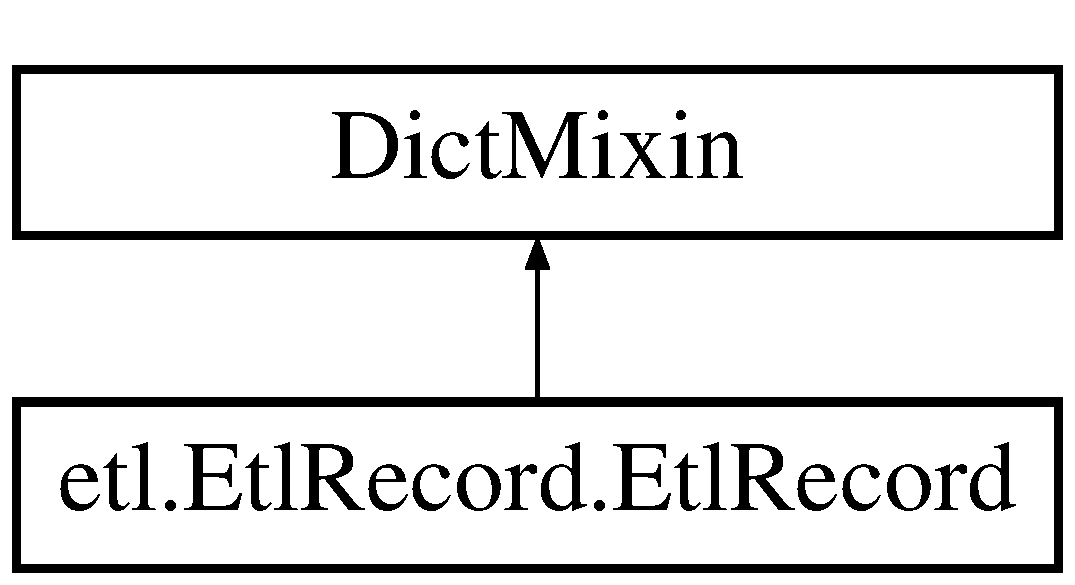
\includegraphics[height=2.000000cm]{classetl_1_1EtlRecord_1_1EtlRecord}
\end{center}
\end{figure}
\subsection*{Public Member Functions}
\begin{DoxyCompactItemize}
\item 
def \hyperlink{classetl_1_1EtlRecord_1_1EtlRecord_a682601780d0d927b8f9dc88e349de18a}{\-\_\-\-\_\-init\-\_\-\-\_\-}
\item 
\hypertarget{classetl_1_1EtlRecord_1_1EtlRecord_a8fe36664b70c30a7f59bd80f09d74e55}{def {\bfseries clone}}\label{classetl_1_1EtlRecord_1_1EtlRecord_a8fe36664b70c30a7f59bd80f09d74e55}

\item 
def \hyperlink{classetl_1_1EtlRecord_1_1EtlRecord_ab73174eafab6b09a253cdb0161f2c895}{serial}
\item 
\hypertarget{classetl_1_1EtlRecord_1_1EtlRecord_a8571d1a2070796be31b369899e514f8e}{def {\bfseries field\-\_\-names}}\label{classetl_1_1EtlRecord_1_1EtlRecord_a8571d1a2070796be31b369899e514f8e}

\item 
def \hyperlink{classetl_1_1EtlRecord_1_1EtlRecord_aada717afc26156c846346af596dcdbb8}{note\-\_\-src\-\_\-record}
\item 
def \hyperlink{classetl_1_1EtlRecord_1_1EtlRecord_a74cfb6726480592e4bc7b7781d82f764}{get\-\_\-src\-\_\-record\-\_\-serials}
\item 
\hypertarget{classetl_1_1EtlRecord_1_1EtlRecord_ab664b0f5cf2ba7abc2e2e31eabf88185}{def {\bfseries set\-\_\-source}}\label{classetl_1_1EtlRecord_1_1EtlRecord_ab664b0f5cf2ba7abc2e2e31eabf88185}

\item 
\hypertarget{classetl_1_1EtlRecord_1_1EtlRecord_ad04be283badfa4f93927d5ee2c028638}{def {\bfseries source\-\_\-processor\-\_\-name}}\label{classetl_1_1EtlRecord_1_1EtlRecord_ad04be283badfa4f93927d5ee2c028638}

\item 
\hypertarget{classetl_1_1EtlRecord_1_1EtlRecord_a11f6d425ebfcc1db3f147431311319ee}{def {\bfseries source\-\_\-processor\-\_\-output\-\_\-name}}\label{classetl_1_1EtlRecord_1_1EtlRecord_a11f6d425ebfcc1db3f147431311319ee}

\item 
def \hyperlink{classetl_1_1EtlRecord_1_1EtlRecord_ac572eae3d8884ccdf3bb3f7f0d6b2717}{create\-\_\-msg}
\item 
\hypertarget{classetl_1_1EtlRecord_1_1EtlRecord_a9b2d840c3032acf5c68d6378caab03c5}{def {\bfseries values}}\label{classetl_1_1EtlRecord_1_1EtlRecord_a9b2d840c3032acf5c68d6378caab03c5}

\item 
\hypertarget{classetl_1_1EtlRecord_1_1EtlRecord_a1e8682345cbb30640c25b075e85ec254}{def {\bfseries value}}\label{classetl_1_1EtlRecord_1_1EtlRecord_a1e8682345cbb30640c25b075e85ec254}

\item 
\hypertarget{classetl_1_1EtlRecord_1_1EtlRecord_a930f84370980ada45f0190bb22a26bda}{def {\bfseries \-\_\-\-\_\-getitem\-\_\-\-\_\-}}\label{classetl_1_1EtlRecord_1_1EtlRecord_a930f84370980ada45f0190bb22a26bda}

\item 
\hypertarget{classetl_1_1EtlRecord_1_1EtlRecord_a83acd0edd9a35ae21b4a6a628a071e04}{def {\bfseries \-\_\-\-\_\-setitem\-\_\-\-\_\-}}\label{classetl_1_1EtlRecord_1_1EtlRecord_a83acd0edd9a35ae21b4a6a628a071e04}

\item 
\hypertarget{classetl_1_1EtlRecord_1_1EtlRecord_a1be42df76a8b623585f4ec44551f47c5}{def {\bfseries set}}\label{classetl_1_1EtlRecord_1_1EtlRecord_a1be42df76a8b623585f4ec44551f47c5}

\item 
\hypertarget{classetl_1_1EtlRecord_1_1EtlRecord_a498f5016e05a25cf95270b6bab207dbc}{def {\bfseries keys}}\label{classetl_1_1EtlRecord_1_1EtlRecord_a498f5016e05a25cf95270b6bab207dbc}

\item 
\hypertarget{classetl_1_1EtlRecord_1_1EtlRecord_abcfc1fc2cd5eea5188a9cf1546b8cc2a}{def {\bfseries freeze}}\label{classetl_1_1EtlRecord_1_1EtlRecord_abcfc1fc2cd5eea5188a9cf1546b8cc2a}

\item 
\hypertarget{classetl_1_1EtlRecord_1_1EtlRecord_a1c6a2552d8cd40357052d72af2f08c03}{def {\bfseries is\-\_\-frozen}}\label{classetl_1_1EtlRecord_1_1EtlRecord_a1c6a2552d8cd40357052d72af2f08c03}

\item 
\hypertarget{classetl_1_1EtlRecord_1_1EtlRecord_a02986930ec9e90a88f7b2ce5bd7b3c35}{def {\bfseries assert\-\_\-not\-\_\-frozen}}\label{classetl_1_1EtlRecord_1_1EtlRecord_a02986930ec9e90a88f7b2ce5bd7b3c35}

\item 
def \hyperlink{classetl_1_1EtlRecord_1_1EtlRecord_a7b4de54d5c2bc343ee1ea8b566702aa4}{size}
\item 
\hypertarget{classetl_1_1EtlRecord_1_1EtlRecord_a2521616e1862aeb072bf164f22ef03d0}{def {\bfseries schema}}\label{classetl_1_1EtlRecord_1_1EtlRecord_a2521616e1862aeb072bf164f22ef03d0}

\item 
def \hyperlink{classetl_1_1EtlRecord_1_1EtlRecord_af51c8ccd4058c0f8307a1cfdc0c86071}{set\-\_\-schema}
\item 
\hypertarget{classetl_1_1EtlRecord_1_1EtlRecord_a26b55f52b15b6d7d9e0d508c0bcadbe6}{def {\bfseries \-\_\-\-\_\-eq\-\_\-\-\_\-}}\label{classetl_1_1EtlRecord_1_1EtlRecord_a26b55f52b15b6d7d9e0d508c0bcadbe6}

\end{DoxyCompactItemize}


\subsection{Detailed Description}
\begin{DoxyVerb}Container for values for a single record

ETL Records are meant to not be mutable once they have been added to an
output set.
\end{DoxyVerb}
 

\subsection{Constructor \& Destructor Documentation}
\hypertarget{classetl_1_1EtlRecord_1_1EtlRecord_a682601780d0d927b8f9dc88e349de18a}{\index{etl\-::\-Etl\-Record\-::\-Etl\-Record@{etl\-::\-Etl\-Record\-::\-Etl\-Record}!\-\_\-\-\_\-init\-\_\-\-\_\-@{\-\_\-\-\_\-init\-\_\-\-\_\-}}
\index{\-\_\-\-\_\-init\-\_\-\-\_\-@{\-\_\-\-\_\-init\-\_\-\-\_\-}!etl::EtlRecord::EtlRecord@{etl\-::\-Etl\-Record\-::\-Etl\-Record}}
\subsubsection[{\-\_\-\-\_\-init\-\_\-\-\_\-}]{\setlength{\rightskip}{0pt plus 5cm}def etl.\-Etl\-Record.\-Etl\-Record.\-\_\-\-\_\-init\-\_\-\-\_\- (
\begin{DoxyParamCaption}
\item[{}]{self, }
\item[{}]{schema, }
\item[{}]{values}
\end{DoxyParamCaption}
)}}\label{classetl_1_1EtlRecord_1_1EtlRecord_a682601780d0d927b8f9dc88e349de18a}
\begin{DoxyVerb}Init

@param schema: The Schema this record is being created to match
@param values: Initial values
\end{DoxyVerb}
 

\subsection{Member Function Documentation}
\hypertarget{classetl_1_1EtlRecord_1_1EtlRecord_ac572eae3d8884ccdf3bb3f7f0d6b2717}{\index{etl\-::\-Etl\-Record\-::\-Etl\-Record@{etl\-::\-Etl\-Record\-::\-Etl\-Record}!create\-\_\-msg@{create\-\_\-msg}}
\index{create\-\_\-msg@{create\-\_\-msg}!etl::EtlRecord::EtlRecord@{etl\-::\-Etl\-Record\-::\-Etl\-Record}}
\subsubsection[{create\-\_\-msg}]{\setlength{\rightskip}{0pt plus 5cm}def etl.\-Etl\-Record.\-Etl\-Record.\-create\-\_\-msg (
\begin{DoxyParamCaption}
\item[{}]{self, }
\item[{}]{msg}
\end{DoxyParamCaption}
)}}\label{classetl_1_1EtlRecord_1_1EtlRecord_ac572eae3d8884ccdf3bb3f7f0d6b2717}
\begin{DoxyVerb}Generate a message about this record\end{DoxyVerb}
 \hypertarget{classetl_1_1EtlRecord_1_1EtlRecord_a74cfb6726480592e4bc7b7781d82f764}{\index{etl\-::\-Etl\-Record\-::\-Etl\-Record@{etl\-::\-Etl\-Record\-::\-Etl\-Record}!get\-\_\-src\-\_\-record\-\_\-serials@{get\-\_\-src\-\_\-record\-\_\-serials}}
\index{get\-\_\-src\-\_\-record\-\_\-serials@{get\-\_\-src\-\_\-record\-\_\-serials}!etl::EtlRecord::EtlRecord@{etl\-::\-Etl\-Record\-::\-Etl\-Record}}
\subsubsection[{get\-\_\-src\-\_\-record\-\_\-serials}]{\setlength{\rightskip}{0pt plus 5cm}def etl.\-Etl\-Record.\-Etl\-Record.\-get\-\_\-src\-\_\-record\-\_\-serials (
\begin{DoxyParamCaption}
\item[{}]{self}
\end{DoxyParamCaption}
)}}\label{classetl_1_1EtlRecord_1_1EtlRecord_a74cfb6726480592e4bc7b7781d82f764}
\begin{DoxyVerb}Serial codes of records that helped generate this record\end{DoxyVerb}
 \hypertarget{classetl_1_1EtlRecord_1_1EtlRecord_aada717afc26156c846346af596dcdbb8}{\index{etl\-::\-Etl\-Record\-::\-Etl\-Record@{etl\-::\-Etl\-Record\-::\-Etl\-Record}!note\-\_\-src\-\_\-record@{note\-\_\-src\-\_\-record}}
\index{note\-\_\-src\-\_\-record@{note\-\_\-src\-\_\-record}!etl::EtlRecord::EtlRecord@{etl\-::\-Etl\-Record\-::\-Etl\-Record}}
\subsubsection[{note\-\_\-src\-\_\-record}]{\setlength{\rightskip}{0pt plus 5cm}def etl.\-Etl\-Record.\-Etl\-Record.\-note\-\_\-src\-\_\-record (
\begin{DoxyParamCaption}
\item[{}]{self, }
\item[{}]{rec}
\end{DoxyParamCaption}
)}}\label{classetl_1_1EtlRecord_1_1EtlRecord_aada717afc26156c846346af596dcdbb8}
\begin{DoxyVerb}Note another record that was processed to help create this record\end{DoxyVerb}
 \hypertarget{classetl_1_1EtlRecord_1_1EtlRecord_ab73174eafab6b09a253cdb0161f2c895}{\index{etl\-::\-Etl\-Record\-::\-Etl\-Record@{etl\-::\-Etl\-Record\-::\-Etl\-Record}!serial@{serial}}
\index{serial@{serial}!etl::EtlRecord::EtlRecord@{etl\-::\-Etl\-Record\-::\-Etl\-Record}}
\subsubsection[{serial}]{\setlength{\rightskip}{0pt plus 5cm}def etl.\-Etl\-Record.\-Etl\-Record.\-serial (
\begin{DoxyParamCaption}
\item[{}]{self}
\end{DoxyParamCaption}
)}}\label{classetl_1_1EtlRecord_1_1EtlRecord_ab73174eafab6b09a253cdb0161f2c895}
\begin{DoxyVerb}Unique identification of this record\end{DoxyVerb}
 \hypertarget{classetl_1_1EtlRecord_1_1EtlRecord_af51c8ccd4058c0f8307a1cfdc0c86071}{\index{etl\-::\-Etl\-Record\-::\-Etl\-Record@{etl\-::\-Etl\-Record\-::\-Etl\-Record}!set\-\_\-schema@{set\-\_\-schema}}
\index{set\-\_\-schema@{set\-\_\-schema}!etl::EtlRecord::EtlRecord@{etl\-::\-Etl\-Record\-::\-Etl\-Record}}
\subsubsection[{set\-\_\-schema}]{\setlength{\rightskip}{0pt plus 5cm}def etl.\-Etl\-Record.\-Etl\-Record.\-set\-\_\-schema (
\begin{DoxyParamCaption}
\item[{}]{self, }
\item[{}]{new\-\_\-schema}
\end{DoxyParamCaption}
)}}\label{classetl_1_1EtlRecord_1_1EtlRecord_af51c8ccd4058c0f8307a1cfdc0c86071}
\begin{DoxyVerb}Replace schema

Note: We allow the schema to be replaced to assist with storing to disk
\end{DoxyVerb}
 \hypertarget{classetl_1_1EtlRecord_1_1EtlRecord_a7b4de54d5c2bc343ee1ea8b566702aa4}{\index{etl\-::\-Etl\-Record\-::\-Etl\-Record@{etl\-::\-Etl\-Record\-::\-Etl\-Record}!size@{size}}
\index{size@{size}!etl::EtlRecord::EtlRecord@{etl\-::\-Etl\-Record\-::\-Etl\-Record}}
\subsubsection[{size}]{\setlength{\rightskip}{0pt plus 5cm}def etl.\-Etl\-Record.\-Etl\-Record.\-size (
\begin{DoxyParamCaption}
\item[{}]{self}
\end{DoxyParamCaption}
)}}\label{classetl_1_1EtlRecord_1_1EtlRecord_a7b4de54d5c2bc343ee1ea8b566702aa4}
\begin{DoxyVerb}Estimate records size\end{DoxyVerb}
 

The documentation for this class was generated from the following file\-:\begin{DoxyCompactItemize}
\item 
src/etl/Etl\-Record.\-py\end{DoxyCompactItemize}

\hypertarget{classetl_1_1EtlRecord_1_1EtlRecordFrozen}{\section{etl.\-Etl\-Record.\-Etl\-Record\-Frozen Class Reference}
\label{classetl_1_1EtlRecord_1_1EtlRecordFrozen}\index{etl.\-Etl\-Record.\-Etl\-Record\-Frozen@{etl.\-Etl\-Record.\-Etl\-Record\-Frozen}}
}
Inheritance diagram for etl.\-Etl\-Record.\-Etl\-Record\-Frozen\-:\begin{figure}[H]
\begin{center}
\leavevmode
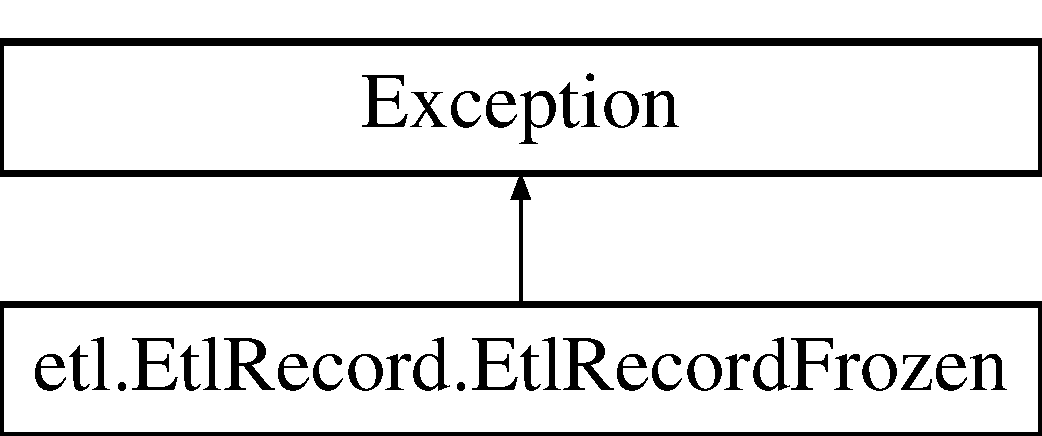
\includegraphics[height=2.000000cm]{classetl_1_1EtlRecord_1_1EtlRecordFrozen}
\end{center}
\end{figure}
\subsection*{Public Member Functions}
\begin{DoxyCompactItemize}
\item 
\hypertarget{classetl_1_1EtlRecord_1_1EtlRecordFrozen_aa79c626e5b00509f1227f6d9cbcc78c7}{def {\bfseries \-\_\-\-\_\-init\-\_\-\-\_\-}}\label{classetl_1_1EtlRecord_1_1EtlRecordFrozen_aa79c626e5b00509f1227f6d9cbcc78c7}

\end{DoxyCompactItemize}


The documentation for this class was generated from the following file\-:\begin{DoxyCompactItemize}
\item 
src/etl/Etl\-Record.\-py\end{DoxyCompactItemize}

\hypertarget{classetl_1_1EtlRecord_1_1EtlRecordSerial}{\section{etl.\-Etl\-Record.\-Etl\-Record\-Serial Class Reference}
\label{classetl_1_1EtlRecord_1_1EtlRecordSerial}\index{etl.\-Etl\-Record.\-Etl\-Record\-Serial@{etl.\-Etl\-Record.\-Etl\-Record\-Serial}}
}
Inheritance diagram for etl.\-Etl\-Record.\-Etl\-Record\-Serial\-:\begin{figure}[H]
\begin{center}
\leavevmode
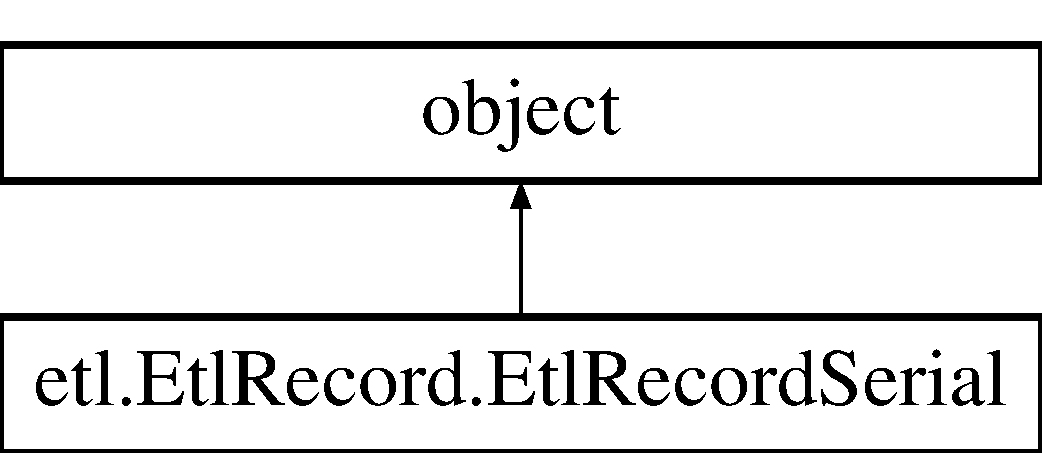
\includegraphics[height=2.000000cm]{classetl_1_1EtlRecord_1_1EtlRecordSerial}
\end{center}
\end{figure}
\subsection*{Public Member Functions}
\begin{DoxyCompactItemize}
\item 
\hypertarget{classetl_1_1EtlRecord_1_1EtlRecordSerial_afe0617aba86f91f92087560d196fedb1}{def {\bfseries \-\_\-\-\_\-init\-\_\-\-\_\-}}\label{classetl_1_1EtlRecord_1_1EtlRecordSerial_afe0617aba86f91f92087560d196fedb1}

\item 
\hypertarget{classetl_1_1EtlRecord_1_1EtlRecordSerial_a61fbf9fc63e6beb391a4daa2c38bb1e7}{def {\bfseries \-\_\-\-\_\-str\-\_\-\-\_\-}}\label{classetl_1_1EtlRecord_1_1EtlRecordSerial_a61fbf9fc63e6beb391a4daa2c38bb1e7}

\item 
\hypertarget{classetl_1_1EtlRecord_1_1EtlRecordSerial_a41e38b3ab463df8ce3e7ce3e876bf59f}{def {\bfseries \-\_\-\-\_\-eq\-\_\-\-\_\-}}\label{classetl_1_1EtlRecord_1_1EtlRecordSerial_a41e38b3ab463df8ce3e7ce3e876bf59f}

\item 
\hypertarget{classetl_1_1EtlRecord_1_1EtlRecordSerial_afe8efc4bd2c8b82802705caf8ded0390}{def {\bfseries \-\_\-\-\_\-hash\-\_\-\-\_\-}}\label{classetl_1_1EtlRecord_1_1EtlRecordSerial_afe8efc4bd2c8b82802705caf8ded0390}

\end{DoxyCompactItemize}


\subsection{Detailed Description}
\begin{DoxyVerb}Unique identification for EtlRecords\end{DoxyVerb}
 

The documentation for this class was generated from the following file\-:\begin{DoxyCompactItemize}
\item 
src/etl/Etl\-Record.\-py\end{DoxyCompactItemize}

\hypertarget{classetl_1_1EtlRecordSet_1_1EtlRecordSet}{\section{etl.\-Etl\-Record\-Set.\-Etl\-Record\-Set Class Reference}
\label{classetl_1_1EtlRecordSet_1_1EtlRecordSet}\index{etl.\-Etl\-Record\-Set.\-Etl\-Record\-Set@{etl.\-Etl\-Record\-Set.\-Etl\-Record\-Set}}
}
Inheritance diagram for etl.\-Etl\-Record\-Set.\-Etl\-Record\-Set\-:\begin{figure}[H]
\begin{center}
\leavevmode
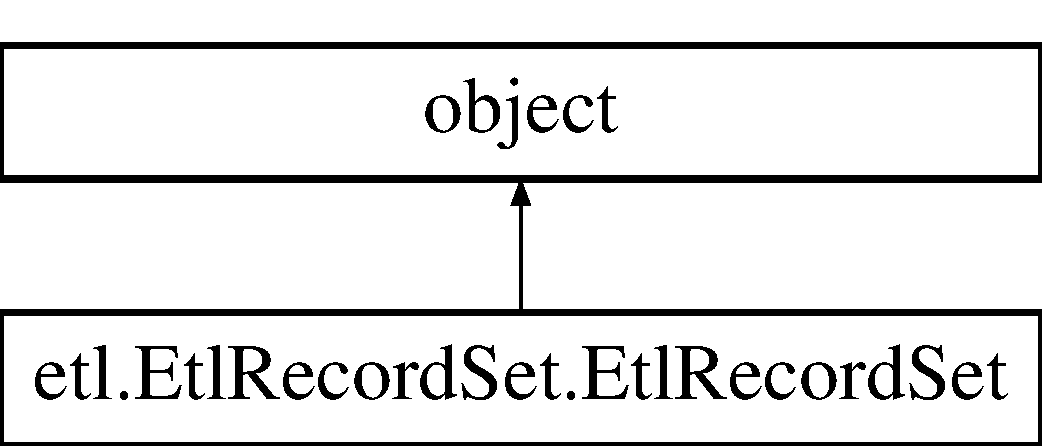
\includegraphics[height=2.000000cm]{classetl_1_1EtlRecordSet_1_1EtlRecordSet}
\end{center}
\end{figure}
\subsection*{Public Member Functions}
\begin{DoxyCompactItemize}
\item 
\hypertarget{classetl_1_1EtlRecordSet_1_1EtlRecordSet_add892dc0a0c458744ff3fd1cc5fc184b}{def {\bfseries \-\_\-\-\_\-init\-\_\-\-\_\-}}\label{classetl_1_1EtlRecordSet_1_1EtlRecordSet_add892dc0a0c458744ff3fd1cc5fc184b}

\item 
def \hyperlink{classetl_1_1EtlRecordSet_1_1EtlRecordSet_a7152530996477950371bd69e9da21298}{add\-\_\-record}
\item 
\hypertarget{classetl_1_1EtlRecordSet_1_1EtlRecordSet_a18701c73a7da83c098ad4b5cdc79741f}{def {\bfseries convert\-\_\-to\-\_\-disk\-\_\-storage}}\label{classetl_1_1EtlRecordSet_1_1EtlRecordSet_a18701c73a7da83c098ad4b5cdc79741f}

\item 
def \hyperlink{classetl_1_1EtlRecordSet_1_1EtlRecordSet_ab01685a2baef3ee4527c005f02122d37}{get\-\_\-record}
\item 
\hypertarget{classetl_1_1EtlRecordSet_1_1EtlRecordSet_aec9eb92e017bccdd3402515c079e8af6}{def {\bfseries has\-\_\-record}}\label{classetl_1_1EtlRecordSet_1_1EtlRecordSet_aec9eb92e017bccdd3402515c079e8af6}

\item 
def \hyperlink{classetl_1_1EtlRecordSet_1_1EtlRecordSet_ab9bfa74fe26ed32b1c6185cb8b7a42c7}{find\-\_\-records\-\_\-with\-\_\-tag}
\item 
\hypertarget{classetl_1_1EtlRecordSet_1_1EtlRecordSet_a51f38f33e821fd3313667b67f7df638d}{def {\bfseries has\-\_\-record\-\_\-with\-\_\-tag}}\label{classetl_1_1EtlRecordSet_1_1EtlRecordSet_a51f38f33e821fd3313667b67f7df638d}

\item 
def \hyperlink{classetl_1_1EtlRecordSet_1_1EtlRecordSet_aceadc74e6289bbe236ee369d5fdde291}{remove\-\_\-record}
\item 
def \hyperlink{classetl_1_1EtlRecordSet_1_1EtlRecordSet_a8bcedcafdc2bafd912eb289335ac129f}{size}
\item 
\hypertarget{classetl_1_1EtlRecordSet_1_1EtlRecordSet_ac7bda13fe8cd3ba9bdd8b3dd3ce6b840}{def {\bfseries count}}\label{classetl_1_1EtlRecordSet_1_1EtlRecordSet_ac7bda13fe8cd3ba9bdd8b3dd3ce6b840}

\item 
\hypertarget{classetl_1_1EtlRecordSet_1_1EtlRecordSet_a0f95a3a7a85b22f50e14ec3e29de83c7}{def {\bfseries on\-\_\-disk}}\label{classetl_1_1EtlRecordSet_1_1EtlRecordSet_a0f95a3a7a85b22f50e14ec3e29de83c7}

\end{DoxyCompactItemize}
\subsection*{Public Attributes}
\begin{DoxyCompactItemize}
\item 
\hypertarget{classetl_1_1EtlRecordSet_1_1EtlRecordSet_aca88b5e66d61ff58dfc9c1265dcff8d7}{{\bfseries max\-\_\-size\-\_\-until\-\_\-disk}}\label{classetl_1_1EtlRecordSet_1_1EtlRecordSet_aca88b5e66d61ff58dfc9c1265dcff8d7}

\end{DoxyCompactItemize}


\subsection{Detailed Description}
\begin{DoxyVerb}Encapsulate a set of records

This object can be used to store multiple records.  If the volume stays
small (under a configurable limit) the records will be stored in memory.
If, however, the number of records based on estimated record size, then
the records will be moved off to disk.

Additionally, indexes can be added for retrieving records by values other
than the record serial
\end{DoxyVerb}
 

\subsection{Member Function Documentation}
\hypertarget{classetl_1_1EtlRecordSet_1_1EtlRecordSet_a7152530996477950371bd69e9da21298}{\index{etl\-::\-Etl\-Record\-Set\-::\-Etl\-Record\-Set@{etl\-::\-Etl\-Record\-Set\-::\-Etl\-Record\-Set}!add\-\_\-record@{add\-\_\-record}}
\index{add\-\_\-record@{add\-\_\-record}!etl::EtlRecordSet::EtlRecordSet@{etl\-::\-Etl\-Record\-Set\-::\-Etl\-Record\-Set}}
\subsubsection[{add\-\_\-record}]{\setlength{\rightskip}{0pt plus 5cm}def etl.\-Etl\-Record\-Set.\-Etl\-Record\-Set.\-add\-\_\-record (
\begin{DoxyParamCaption}
\item[{}]{self, }
\item[{}]{etl\-\_\-rec, }
\item[{}]{tags = {\ttfamily None}}
\end{DoxyParamCaption}
)}}\label{classetl_1_1EtlRecordSet_1_1EtlRecordSet_a7152530996477950371bd69e9da21298}
\begin{DoxyVerb}Add a record to the collection

Use indexes to index this 

@param etl_rec: Record to store
@param tags: List of optional additional tags to be used for retrieving
    this record.  Record must be convertible to a string with str()
\end{DoxyVerb}
 \hypertarget{classetl_1_1EtlRecordSet_1_1EtlRecordSet_ab9bfa74fe26ed32b1c6185cb8b7a42c7}{\index{etl\-::\-Etl\-Record\-Set\-::\-Etl\-Record\-Set@{etl\-::\-Etl\-Record\-Set\-::\-Etl\-Record\-Set}!find\-\_\-records\-\_\-with\-\_\-tag@{find\-\_\-records\-\_\-with\-\_\-tag}}
\index{find\-\_\-records\-\_\-with\-\_\-tag@{find\-\_\-records\-\_\-with\-\_\-tag}!etl::EtlRecordSet::EtlRecordSet@{etl\-::\-Etl\-Record\-Set\-::\-Etl\-Record\-Set}}
\subsubsection[{find\-\_\-records\-\_\-with\-\_\-tag}]{\setlength{\rightskip}{0pt plus 5cm}def etl.\-Etl\-Record\-Set.\-Etl\-Record\-Set.\-find\-\_\-records\-\_\-with\-\_\-tag (
\begin{DoxyParamCaption}
\item[{}]{self, }
\item[{}]{tag}
\end{DoxyParamCaption}
)}}\label{classetl_1_1EtlRecordSet_1_1EtlRecordSet_ab9bfa74fe26ed32b1c6185cb8b7a42c7}
\begin{DoxyVerb}Find records that have a given tag\end{DoxyVerb}
 \hypertarget{classetl_1_1EtlRecordSet_1_1EtlRecordSet_ab01685a2baef3ee4527c005f02122d37}{\index{etl\-::\-Etl\-Record\-Set\-::\-Etl\-Record\-Set@{etl\-::\-Etl\-Record\-Set\-::\-Etl\-Record\-Set}!get\-\_\-record@{get\-\_\-record}}
\index{get\-\_\-record@{get\-\_\-record}!etl::EtlRecordSet::EtlRecordSet@{etl\-::\-Etl\-Record\-Set\-::\-Etl\-Record\-Set}}
\subsubsection[{get\-\_\-record}]{\setlength{\rightskip}{0pt plus 5cm}def etl.\-Etl\-Record\-Set.\-Etl\-Record\-Set.\-get\-\_\-record (
\begin{DoxyParamCaption}
\item[{}]{self, }
\item[{}]{serial}
\end{DoxyParamCaption}
)}}\label{classetl_1_1EtlRecordSet_1_1EtlRecordSet_ab01685a2baef3ee4527c005f02122d37}
\begin{DoxyVerb}Retrieve a record

@param serical:
    Record identifier
@return EtlRecord
\end{DoxyVerb}
 \hypertarget{classetl_1_1EtlRecordSet_1_1EtlRecordSet_aceadc74e6289bbe236ee369d5fdde291}{\index{etl\-::\-Etl\-Record\-Set\-::\-Etl\-Record\-Set@{etl\-::\-Etl\-Record\-Set\-::\-Etl\-Record\-Set}!remove\-\_\-record@{remove\-\_\-record}}
\index{remove\-\_\-record@{remove\-\_\-record}!etl::EtlRecordSet::EtlRecordSet@{etl\-::\-Etl\-Record\-Set\-::\-Etl\-Record\-Set}}
\subsubsection[{remove\-\_\-record}]{\setlength{\rightskip}{0pt plus 5cm}def etl.\-Etl\-Record\-Set.\-Etl\-Record\-Set.\-remove\-\_\-record (
\begin{DoxyParamCaption}
\item[{}]{self, }
\item[{}]{serial}
\end{DoxyParamCaption}
)}}\label{classetl_1_1EtlRecordSet_1_1EtlRecordSet_aceadc74e6289bbe236ee369d5fdde291}
\begin{DoxyVerb}Drop a record from the collection\end{DoxyVerb}
 \hypertarget{classetl_1_1EtlRecordSet_1_1EtlRecordSet_a8bcedcafdc2bafd912eb289335ac129f}{\index{etl\-::\-Etl\-Record\-Set\-::\-Etl\-Record\-Set@{etl\-::\-Etl\-Record\-Set\-::\-Etl\-Record\-Set}!size@{size}}
\index{size@{size}!etl::EtlRecordSet::EtlRecordSet@{etl\-::\-Etl\-Record\-Set\-::\-Etl\-Record\-Set}}
\subsubsection[{size}]{\setlength{\rightskip}{0pt plus 5cm}def etl.\-Etl\-Record\-Set.\-Etl\-Record\-Set.\-size (
\begin{DoxyParamCaption}
\item[{}]{self}
\end{DoxyParamCaption}
)}}\label{classetl_1_1EtlRecordSet_1_1EtlRecordSet_a8bcedcafdc2bafd912eb289335ac129f}
\begin{DoxyVerb}Estimated size of the record set\end{DoxyVerb}
 

The documentation for this class was generated from the following file\-:\begin{DoxyCompactItemize}
\item 
src/etl/Etl\-Record\-Set.\-py\end{DoxyCompactItemize}

\hypertarget{classetl_1_1EtlWorkflow_1_1EtlWorkflow}{\section{etl.\-Etl\-Workflow.\-Etl\-Workflow Class Reference}
\label{classetl_1_1EtlWorkflow_1_1EtlWorkflow}\index{etl.\-Etl\-Workflow.\-Etl\-Workflow@{etl.\-Etl\-Workflow.\-Etl\-Workflow}}
}
Inheritance diagram for etl.\-Etl\-Workflow.\-Etl\-Workflow\-:\begin{figure}[H]
\begin{center}
\leavevmode
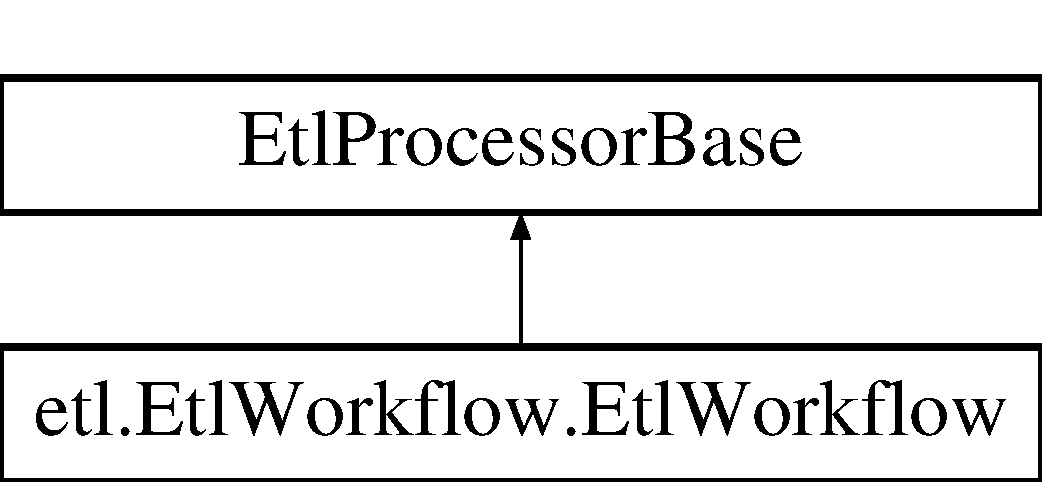
\includegraphics[height=2.000000cm]{classetl_1_1EtlWorkflow_1_1EtlWorkflow}
\end{center}
\end{figure}
\subsection*{Public Member Functions}
\begin{DoxyCompactItemize}
\item 
\hypertarget{classetl_1_1EtlWorkflow_1_1EtlWorkflow_a1966fd97419f8ccaf6363c4b05fbce3c}{def {\bfseries \-\_\-\-\_\-init\-\_\-\-\_\-}}\label{classetl_1_1EtlWorkflow_1_1EtlWorkflow_a1966fd97419f8ccaf6363c4b05fbce3c}

\item 
def \hyperlink{classetl_1_1EtlWorkflow_1_1EtlWorkflow_a0027ab0811e6b677f28ca6d58f28f823}{add\-\_\-processor}
\item 
def \hyperlink{classetl_1_1EtlWorkflow_1_1EtlWorkflow_a008c9d5aafebcce7b0aab326b1c51e6b}{connect}
\item 
def \hyperlink{classetl_1_1EtlWorkflow_1_1EtlWorkflow_a4f71423ab6481714ba85cfe16291bd42}{execute}
\item 
def \hyperlink{classetl_1_1EtlWorkflow_1_1EtlWorkflow_aae398dcde51ad92c1592a548f71657b6}{save\-\_\-records}
\item 
\hypertarget{classetl_1_1EtlWorkflow_1_1EtlWorkflow_a85e71dd38d728fbe563577f38d332c29}{def {\bfseries list\-\_\-prc\-\_\-names}}\label{classetl_1_1EtlWorkflow_1_1EtlWorkflow_a85e71dd38d728fbe563577f38d332c29}

\item 
\hypertarget{classetl_1_1EtlWorkflow_1_1EtlWorkflow_a9f0f6e2d6be094538942928106c1f180}{def {\bfseries get\-\_\-prc}}\label{classetl_1_1EtlWorkflow_1_1EtlWorkflow_a9f0f6e2d6be094538942928106c1f180}

\end{DoxyCompactItemize}
\subsection*{Public Attributes}
\begin{DoxyCompactItemize}
\item 
\hypertarget{classetl_1_1EtlWorkflow_1_1EtlWorkflow_a331fee0c614841321d0fb719a58f7135}{{\bfseries default\-\_\-data\-\_\-directory}}\label{classetl_1_1EtlWorkflow_1_1EtlWorkflow_a331fee0c614841321d0fb719a58f7135}

\item 
\hypertarget{classetl_1_1EtlWorkflow_1_1EtlWorkflow_a9f952af1fcc8d93985c84c83485318e0}{{\bfseries temp\-\_\-directory}}\label{classetl_1_1EtlWorkflow_1_1EtlWorkflow_a9f952af1fcc8d93985c84c83485318e0}

\end{DoxyCompactItemize}


\subsection{Detailed Description}
\begin{DoxyVerb}Encapsulates an ETL workflow

This class is used to organize all of the components in the workflow.
It is itself a processor in the ETL Workflow, refered to as the root
processor.  Unlike child processors based on EtlProcessor, though,
this root processor runs in the same thread as the invoking code.

Definition of ETL:
------------------
from [Wikipedia](http://en.wikipedia.org/wiki/Extract,_transform,_load)

In computing, Extract, Transform and Load (ETL) refers to a process in
database usage and especially in data warehousing that:

Extracts data from homogeneous or heterogeneous data sources Transforms the
data for storing it in proper format or structure for querying and analysis
purpose Loads it into the final target (database, more specifically,
operational data store, data mart, or data warehouse) Usually all the three
phases execute in parallel since the data extraction takes time, so while
the data is being pulled another transformation process executes, processing
the already received data and prepares the data for loading and as soon as
there is some data ready to be loaded into the target, the data loading
kicks off without waiting for the completion of the previous phases.

ETL systems commonly integrate data from multiple applications(systems),
typically developed and supported by different vendors or hosted on separate
computer hardware. The disparate systems containing the original data are
frequently managed and operated by different employees. For example a cost
accounting system may combine data from payroll, sales and purchasing.


Creating an ETL Process
-----------------------

In order to define an ETL process, the developer is encouraged to
subclass this class and then define and connect the processors.
This class does not need to be subclassed to create an ETL process,
though, as you can just instantiate it and call the methods.

 1) Define your processors by subclassing EtlProcessor, or using the
    common processors under etl.common

 2) Call add_processor() to add your processors to the Workflow

 3) Call connect() to connect the output ports of processors to the
    input ports of other processors

 4) Call assign_processor_output() to connect the output ports of
    processors to an input port of this Workflow object.  This allows
    you to define a path for records to exit the ETL workflow and
    be returned to the calling code.  When you call the workflow.
    execute() method to run the ETL process, and records dispatched
    on the specified port will be yielded back to the calling function.

  5) Call exectue() - Run the workflow to generate the desired output. 
\end{DoxyVerb}
 

\subsection{Member Function Documentation}
\hypertarget{classetl_1_1EtlWorkflow_1_1EtlWorkflow_a0027ab0811e6b677f28ca6d58f28f823}{\index{etl\-::\-Etl\-Workflow\-::\-Etl\-Workflow@{etl\-::\-Etl\-Workflow\-::\-Etl\-Workflow}!add\-\_\-processor@{add\-\_\-processor}}
\index{add\-\_\-processor@{add\-\_\-processor}!etl::EtlWorkflow::EtlWorkflow@{etl\-::\-Etl\-Workflow\-::\-Etl\-Workflow}}
\subsubsection[{add\-\_\-processor}]{\setlength{\rightskip}{0pt plus 5cm}def etl.\-Etl\-Workflow.\-Etl\-Workflow.\-add\-\_\-processor (
\begin{DoxyParamCaption}
\item[{}]{self, }
\item[{}]{name, }
\item[{}]{prc}
\end{DoxyParamCaption}
)}}\label{classetl_1_1EtlWorkflow_1_1EtlWorkflow_a0027ab0811e6b677f28ca6d58f28f823}
\begin{DoxyVerb}Add a processor to the workflow

@param name: Name to identify this processor
@param prc: EtlProcessor class
\end{DoxyVerb}
 \hypertarget{classetl_1_1EtlWorkflow_1_1EtlWorkflow_a008c9d5aafebcce7b0aab326b1c51e6b}{\index{etl\-::\-Etl\-Workflow\-::\-Etl\-Workflow@{etl\-::\-Etl\-Workflow\-::\-Etl\-Workflow}!connect@{connect}}
\index{connect@{connect}!etl::EtlWorkflow::EtlWorkflow@{etl\-::\-Etl\-Workflow\-::\-Etl\-Workflow}}
\subsubsection[{connect}]{\setlength{\rightskip}{0pt plus 5cm}def etl.\-Etl\-Workflow.\-Etl\-Workflow.\-connect (
\begin{DoxyParamCaption}
\item[{}]{self, }
\item[{}]{from\-\_\-prc\-\_\-name, }
\item[{}]{output\-\_\-name, }
\item[{}]{to\-\_\-prc\-\_\-name, }
\item[{}]{input\-\_\-name = {\ttfamily None}}
\end{DoxyParamCaption}
)}}\label{classetl_1_1EtlWorkflow_1_1EtlWorkflow_a008c9d5aafebcce7b0aab326b1c51e6b}
\begin{DoxyVerb}Connect the output from one processor to the input of another

@param from_prc_name: Name of processor producing data
@param output_name: Name identifying dataset generated by from_prc
@param to_prc_name: Name of processor consuming data
@param input_name: Name of input port on to_prc to provide data on
\end{DoxyVerb}
 \hypertarget{classetl_1_1EtlWorkflow_1_1EtlWorkflow_a4f71423ab6481714ba85cfe16291bd42}{\index{etl\-::\-Etl\-Workflow\-::\-Etl\-Workflow@{etl\-::\-Etl\-Workflow\-::\-Etl\-Workflow}!execute@{execute}}
\index{execute@{execute}!etl::EtlWorkflow::EtlWorkflow@{etl\-::\-Etl\-Workflow\-::\-Etl\-Workflow}}
\subsubsection[{execute}]{\setlength{\rightskip}{0pt plus 5cm}def etl.\-Etl\-Workflow.\-Etl\-Workflow.\-execute (
\begin{DoxyParamCaption}
\item[{}]{self, }
\item[{}]{prc\-\_\-name}
\end{DoxyParamCaption}
)}}\label{classetl_1_1EtlWorkflow_1_1EtlWorkflow_a4f71423ab6481714ba85cfe16291bd42}
\begin{DoxyVerb}Execute the processor (and any dependency processors) and return\end{DoxyVerb}
 \hypertarget{classetl_1_1EtlWorkflow_1_1EtlWorkflow_aae398dcde51ad92c1592a548f71657b6}{\index{etl\-::\-Etl\-Workflow\-::\-Etl\-Workflow@{etl\-::\-Etl\-Workflow\-::\-Etl\-Workflow}!save\-\_\-records@{save\-\_\-records}}
\index{save\-\_\-records@{save\-\_\-records}!etl::EtlWorkflow::EtlWorkflow@{etl\-::\-Etl\-Workflow\-::\-Etl\-Workflow}}
\subsubsection[{save\-\_\-records}]{\setlength{\rightskip}{0pt plus 5cm}def etl.\-Etl\-Workflow.\-Etl\-Workflow.\-save\-\_\-records (
\begin{DoxyParamCaption}
\item[{}]{self, }
\item[{}]{prc\-\_\-name, }
\item[{}]{output\-\_\-name, }
\item[{}]{filename}
\end{DoxyParamCaption}
)}}\label{classetl_1_1EtlWorkflow_1_1EtlWorkflow_aae398dcde51ad92c1592a548f71657b6}
\begin{DoxyVerb}Output records to a file from a processor for review\end{DoxyVerb}
 

The documentation for this class was generated from the following file\-:\begin{DoxyCompactItemize}
\item 
src/etl/Etl\-Workflow.\-py\end{DoxyCompactItemize}

\hypertarget{classetl_1_1exceptions_1_1EtlBuildError}{\section{etl.\-exceptions.\-Etl\-Build\-Error Class Reference}
\label{classetl_1_1exceptions_1_1EtlBuildError}\index{etl.\-exceptions.\-Etl\-Build\-Error@{etl.\-exceptions.\-Etl\-Build\-Error}}
}
Inheritance diagram for etl.\-exceptions.\-Etl\-Build\-Error\-:\begin{figure}[H]
\begin{center}
\leavevmode
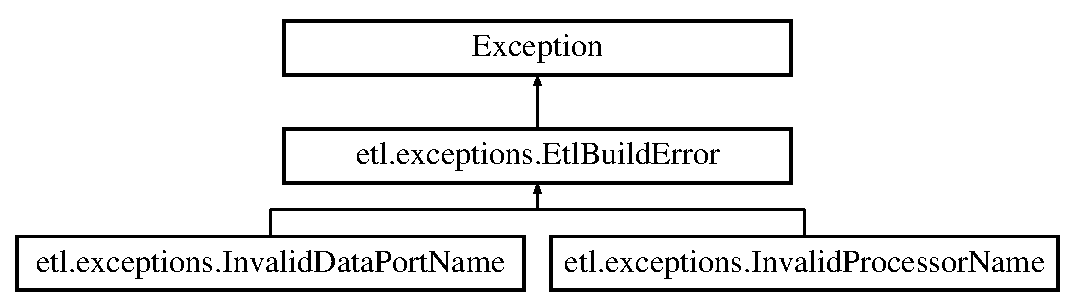
\includegraphics[height=3.000000cm]{classetl_1_1exceptions_1_1EtlBuildError}
\end{center}
\end{figure}
\subsection*{Public Member Functions}
\begin{DoxyCompactItemize}
\item 
def \hyperlink{classetl_1_1exceptions_1_1EtlBuildError_a4bc99a9d770dfa025deaa8f470181731}{\-\_\-\-\_\-init\-\_\-\-\_\-}
\item 
\hypertarget{classetl_1_1exceptions_1_1EtlBuildError_a6e6d78ffbbab68ef638a7a54cf3996f6}{def {\bfseries get\-\_\-prc\-\_\-desc}}\label{classetl_1_1exceptions_1_1EtlBuildError_a6e6d78ffbbab68ef638a7a54cf3996f6}

\item 
\hypertarget{classetl_1_1exceptions_1_1EtlBuildError_ac0dbb3448b32b9f49e070e46b555926a}{def {\bfseries print\-\_\-std\-\_\-error}}\label{classetl_1_1exceptions_1_1EtlBuildError_ac0dbb3448b32b9f49e070e46b555926a}

\end{DoxyCompactItemize}
\subsection*{Public Attributes}
\begin{DoxyCompactItemize}
\item 
\hypertarget{classetl_1_1exceptions_1_1EtlBuildError_a95176d74ba9649f6f5736c3a4cf5ec2d}{{\bfseries prc\-\_\-name}}\label{classetl_1_1exceptions_1_1EtlBuildError_a95176d74ba9649f6f5736c3a4cf5ec2d}

\item 
\hypertarget{classetl_1_1exceptions_1_1EtlBuildError_a1ed55d1a80852a9b934e82bfa93eb84d}{{\bfseries prc\-\_\-class\-\_\-name}}\label{classetl_1_1exceptions_1_1EtlBuildError_a1ed55d1a80852a9b934e82bfa93eb84d}

\item 
\hypertarget{classetl_1_1exceptions_1_1EtlBuildError_a67a70799f2f796627d37e3f9dd1cb630}{{\bfseries etl\-\_\-build\-\_\-error\-\_\-msg}}\label{classetl_1_1exceptions_1_1EtlBuildError_a67a70799f2f796627d37e3f9dd1cb630}

\item 
\hypertarget{classetl_1_1exceptions_1_1EtlBuildError_ab5977adc46b62cd167e3ad4d74752f76}{{\bfseries possible\-\_\-values}}\label{classetl_1_1exceptions_1_1EtlBuildError_ab5977adc46b62cd167e3ad4d74752f76}

\end{DoxyCompactItemize}


\subsection{Detailed Description}
\begin{DoxyVerb}Error with the structure of the ETL graph\end{DoxyVerb}
 

\subsection{Constructor \& Destructor Documentation}
\hypertarget{classetl_1_1exceptions_1_1EtlBuildError_a4bc99a9d770dfa025deaa8f470181731}{\index{etl\-::exceptions\-::\-Etl\-Build\-Error@{etl\-::exceptions\-::\-Etl\-Build\-Error}!\-\_\-\-\_\-init\-\_\-\-\_\-@{\-\_\-\-\_\-init\-\_\-\-\_\-}}
\index{\-\_\-\-\_\-init\-\_\-\-\_\-@{\-\_\-\-\_\-init\-\_\-\-\_\-}!etl::exceptions::EtlBuildError@{etl\-::exceptions\-::\-Etl\-Build\-Error}}
\subsubsection[{\-\_\-\-\_\-init\-\_\-\-\_\-}]{\setlength{\rightskip}{0pt plus 5cm}def etl.\-exceptions.\-Etl\-Build\-Error.\-\_\-\-\_\-init\-\_\-\-\_\- (
\begin{DoxyParamCaption}
\item[{}]{self, }
\item[{}]{prc\-\_\-name, }
\item[{}]{prc\-\_\-class\-\_\-name, }
\item[{}]{error\-\_\-msg, }
\item[{}]{possible\-\_\-values}
\end{DoxyParamCaption}
)}}\label{classetl_1_1exceptions_1_1EtlBuildError_a4bc99a9d770dfa025deaa8f470181731}
\begin{DoxyVerb}Error with the structure of the ETL graph\end{DoxyVerb}
\begin{DoxyVerb}Init

@param prc_name: Name of the processor in the ETL graph
@param prc_class_name: Processor class name
@param error_msg: Description of the error encountered
@param possible_values: List of correct values that could have been used
\end{DoxyVerb}
 

The documentation for this class was generated from the following file\-:\begin{DoxyCompactItemize}
\item 
src/etl/exceptions.\-py\end{DoxyCompactItemize}

\hypertarget{classetl_1_1exceptions_1_1InvalidDataPortName}{\section{etl.\-exceptions.\-Invalid\-Data\-Port\-Name Class Reference}
\label{classetl_1_1exceptions_1_1InvalidDataPortName}\index{etl.\-exceptions.\-Invalid\-Data\-Port\-Name@{etl.\-exceptions.\-Invalid\-Data\-Port\-Name}}
}
Inheritance diagram for etl.\-exceptions.\-Invalid\-Data\-Port\-Name\-:\begin{figure}[H]
\begin{center}
\leavevmode
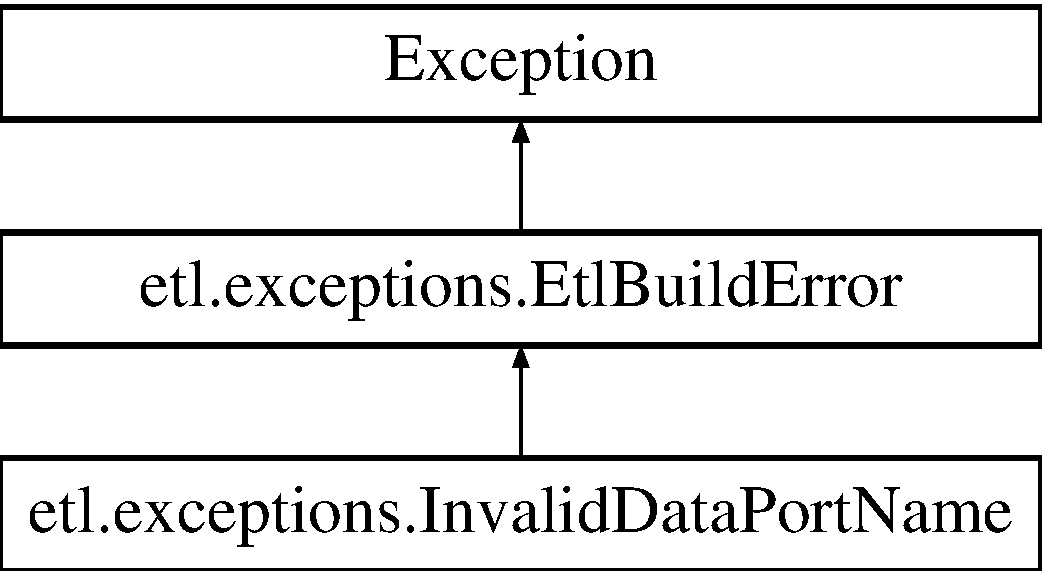
\includegraphics[height=3.000000cm]{classetl_1_1exceptions_1_1InvalidDataPortName}
\end{center}
\end{figure}
\subsection*{Additional Inherited Members}


\subsection{Detailed Description}
\begin{DoxyVerb}A non-existant dataport was referenced for a processor\end{DoxyVerb}
 

The documentation for this class was generated from the following file\-:\begin{DoxyCompactItemize}
\item 
src/etl/exceptions.\-py\end{DoxyCompactItemize}

\hypertarget{classetl_1_1exceptions_1_1InvalidProcessorName}{\section{etl.\-exceptions.\-Invalid\-Processor\-Name Class Reference}
\label{classetl_1_1exceptions_1_1InvalidProcessorName}\index{etl.\-exceptions.\-Invalid\-Processor\-Name@{etl.\-exceptions.\-Invalid\-Processor\-Name}}
}
Inheritance diagram for etl.\-exceptions.\-Invalid\-Processor\-Name\-:\begin{figure}[H]
\begin{center}
\leavevmode
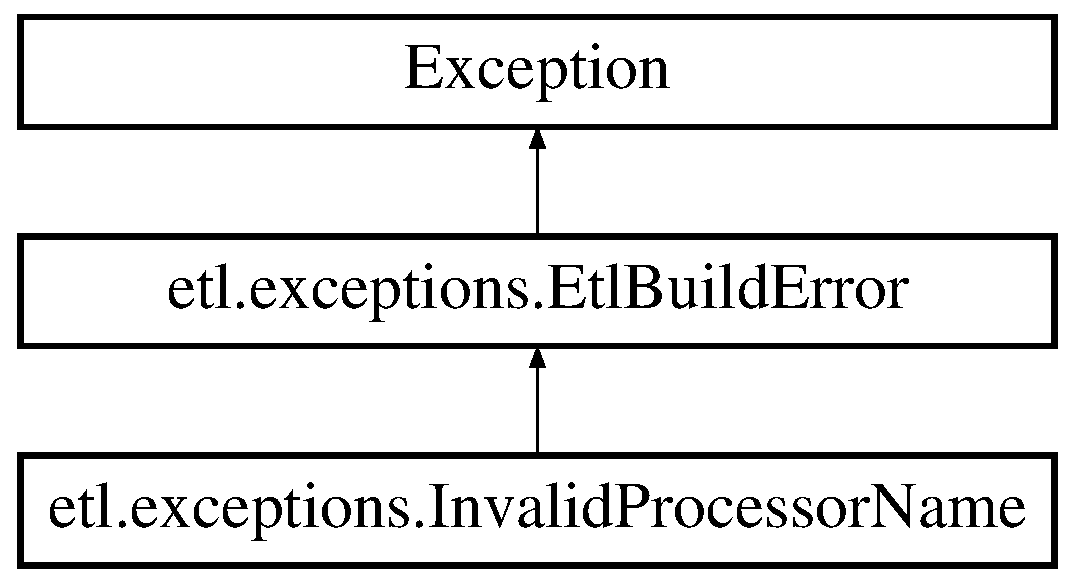
\includegraphics[height=3.000000cm]{classetl_1_1exceptions_1_1InvalidProcessorName}
\end{center}
\end{figure}
\subsection*{Additional Inherited Members}


\subsection{Detailed Description}
\begin{DoxyVerb}A non-existent processor dataport name was used\end{DoxyVerb}
 

The documentation for this class was generated from the following file\-:\begin{DoxyCompactItemize}
\item 
src/etl/exceptions.\-py\end{DoxyCompactItemize}

\hypertarget{classetl_1_1ports_1_1EtlInputConnection}{\section{etl.\-ports.\-Etl\-Input\-Connection Class Reference}
\label{classetl_1_1ports_1_1EtlInputConnection}\index{etl.\-ports.\-Etl\-Input\-Connection@{etl.\-ports.\-Etl\-Input\-Connection}}
}
Inheritance diagram for etl.\-ports.\-Etl\-Input\-Connection\-:\begin{figure}[H]
\begin{center}
\leavevmode
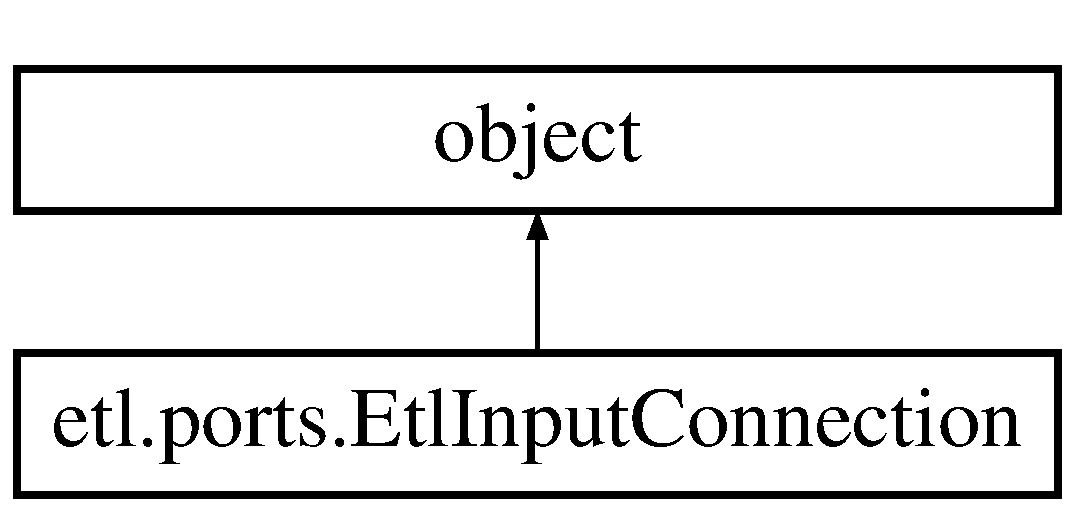
\includegraphics[height=2.000000cm]{classetl_1_1ports_1_1EtlInputConnection}
\end{center}
\end{figure}
\subsection*{Public Member Functions}
\begin{DoxyCompactItemize}
\item 
\hypertarget{classetl_1_1ports_1_1EtlInputConnection_a3bbacdfad36e5944e39eb33202434486}{def {\bfseries \-\_\-\-\_\-init\-\_\-\-\_\-}}\label{classetl_1_1ports_1_1EtlInputConnection_a3bbacdfad36e5944e39eb33202434486}

\end{DoxyCompactItemize}
\subsection*{Public Attributes}
\begin{DoxyCompactItemize}
\item 
\hypertarget{classetl_1_1ports_1_1EtlInputConnection_ab93181d0d0fbfb7438fb9cf242a08b50}{{\bfseries conn\-\_\-id}}\label{classetl_1_1ports_1_1EtlInputConnection_ab93181d0d0fbfb7438fb9cf242a08b50}

\item 
\hypertarget{classetl_1_1ports_1_1EtlInputConnection_aaec9231f33d131f6ff0ae4e319253f58}{{\bfseries status}}\label{classetl_1_1ports_1_1EtlInputConnection_aaec9231f33d131f6ff0ae4e319253f58}

\item 
\hypertarget{classetl_1_1ports_1_1EtlInputConnection_a8223fa4ed1d57909f95af7b9cb2d27fc}{{\bfseries prc\-\_\-name}}\label{classetl_1_1ports_1_1EtlInputConnection_a8223fa4ed1d57909f95af7b9cb2d27fc}

\item 
\hypertarget{classetl_1_1ports_1_1EtlInputConnection_a91fbf1b0ae7d316e3dd47519d831f087}{{\bfseries port\-\_\-name}}\label{classetl_1_1ports_1_1EtlInputConnection_a91fbf1b0ae7d316e3dd47519d831f087}

\item 
\hypertarget{classetl_1_1ports_1_1EtlInputConnection_a8243b6dc6d8243f8ffd166cc44d9135a}{{\bfseries schema}}\label{classetl_1_1ports_1_1EtlInputConnection_a8243b6dc6d8243f8ffd166cc44d9135a}

\end{DoxyCompactItemize}


\subsection{Detailed Description}
\begin{DoxyVerb}Holds details about a manager connected to an input\end{DoxyVerb}
 

The documentation for this class was generated from the following file\-:\begin{DoxyCompactItemize}
\item 
src/etl/ports.\-py\end{DoxyCompactItemize}

\hypertarget{classetl_1_1ports_1_1EtlOutputConnection}{\section{etl.\-ports.\-Etl\-Output\-Connection Class Reference}
\label{classetl_1_1ports_1_1EtlOutputConnection}\index{etl.\-ports.\-Etl\-Output\-Connection@{etl.\-ports.\-Etl\-Output\-Connection}}
}
Inheritance diagram for etl.\-ports.\-Etl\-Output\-Connection\-:\begin{figure}[H]
\begin{center}
\leavevmode
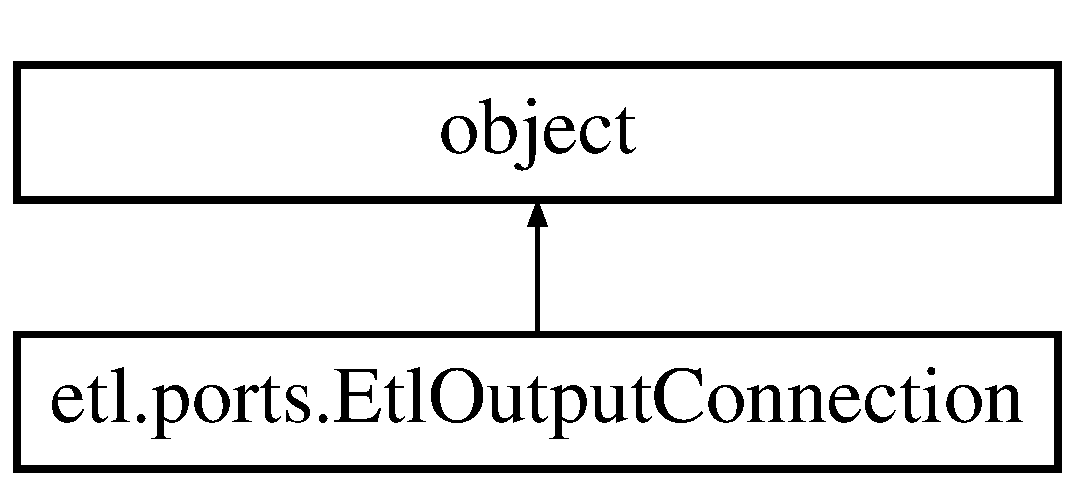
\includegraphics[height=2.000000cm]{classetl_1_1ports_1_1EtlOutputConnection}
\end{center}
\end{figure}
\subsection*{Public Member Functions}
\begin{DoxyCompactItemize}
\item 
def \hyperlink{classetl_1_1ports_1_1EtlOutputConnection_a1f26d4991f7787e9b8b83acb0aedfba7}{\-\_\-\-\_\-init\-\_\-\-\_\-}
\end{DoxyCompactItemize}
\subsection*{Public Attributes}
\begin{DoxyCompactItemize}
\item 
\hypertarget{classetl_1_1ports_1_1EtlOutputConnection_a771e02171336dd965ae7eee643eb7b9c}{{\bfseries status}}\label{classetl_1_1ports_1_1EtlOutputConnection_a771e02171336dd965ae7eee643eb7b9c}

\item 
\hypertarget{classetl_1_1ports_1_1EtlOutputConnection_a34218924437303c38d534aa1465ab274}{{\bfseries target\-\_\-prc\-\_\-name}}\label{classetl_1_1ports_1_1EtlOutputConnection_a34218924437303c38d534aa1465ab274}

\item 
\hypertarget{classetl_1_1ports_1_1EtlOutputConnection_a1a4934ecc7241bd2f5038403a858b7ea}{{\bfseries target\-\_\-prc}}\label{classetl_1_1ports_1_1EtlOutputConnection_a1a4934ecc7241bd2f5038403a858b7ea}

\item 
\hypertarget{classetl_1_1ports_1_1EtlOutputConnection_a7f2dfe89cd05379cb190344c6f512809}{{\bfseries target\-\_\-prc\-\_\-port\-\_\-name}}\label{classetl_1_1ports_1_1EtlOutputConnection_a7f2dfe89cd05379cb190344c6f512809}

\item 
\hypertarget{classetl_1_1ports_1_1EtlOutputConnection_aa465f6a3efc401182008bc832e3f26df}{{\bfseries prc\-\_\-manager}}\label{classetl_1_1ports_1_1EtlOutputConnection_aa465f6a3efc401182008bc832e3f26df}

\item 
\hypertarget{classetl_1_1ports_1_1EtlOutputConnection_aa74f8e59c37366b2fa9d872dd9cba2f2}{{\bfseries schema}}\label{classetl_1_1ports_1_1EtlOutputConnection_aa74f8e59c37366b2fa9d872dd9cba2f2}

\item 
\hypertarget{classetl_1_1ports_1_1EtlOutputConnection_ab923f043e03fed689666370375cbd697}{{\bfseries event\-\_\-queue}}\label{classetl_1_1ports_1_1EtlOutputConnection_ab923f043e03fed689666370375cbd697}

\item 
\hypertarget{classetl_1_1ports_1_1EtlOutputConnection_a4562dedc4777fd516e563293b60d3586}{{\bfseries record\-\_\-queue}}\label{classetl_1_1ports_1_1EtlOutputConnection_a4562dedc4777fd516e563293b60d3586}

\end{DoxyCompactItemize}


\subsection{Detailed Description}
\begin{DoxyVerb}Holds details about a connection to another processor's input port\end{DoxyVerb}
 

\subsection{Constructor \& Destructor Documentation}
\hypertarget{classetl_1_1ports_1_1EtlOutputConnection_a1f26d4991f7787e9b8b83acb0aedfba7}{\index{etl\-::ports\-::\-Etl\-Output\-Connection@{etl\-::ports\-::\-Etl\-Output\-Connection}!\-\_\-\-\_\-init\-\_\-\-\_\-@{\-\_\-\-\_\-init\-\_\-\-\_\-}}
\index{\-\_\-\-\_\-init\-\_\-\-\_\-@{\-\_\-\-\_\-init\-\_\-\-\_\-}!etl::ports::EtlOutputConnection@{etl\-::ports\-::\-Etl\-Output\-Connection}}
\subsubsection[{\-\_\-\-\_\-init\-\_\-\-\_\-}]{\setlength{\rightskip}{0pt plus 5cm}def etl.\-ports.\-Etl\-Output\-Connection.\-\_\-\-\_\-init\-\_\-\-\_\- (
\begin{DoxyParamCaption}
\item[{}]{self}
\end{DoxyParamCaption}
)}}\label{classetl_1_1ports_1_1EtlOutputConnection_a1f26d4991f7787e9b8b83acb0aedfba7}
\begin{DoxyVerb}Holds details about a connection to another processor's input port\end{DoxyVerb}
 

The documentation for this class was generated from the following file\-:\begin{DoxyCompactItemize}
\item 
src/etl/ports.\-py\end{DoxyCompactItemize}

\hypertarget{classetl_1_1ports_1_1InputPort}{\section{etl.\-ports.\-Input\-Port Class Reference}
\label{classetl_1_1ports_1_1InputPort}\index{etl.\-ports.\-Input\-Port@{etl.\-ports.\-Input\-Port}}
}
Inheritance diagram for etl.\-ports.\-Input\-Port\-:\begin{figure}[H]
\begin{center}
\leavevmode
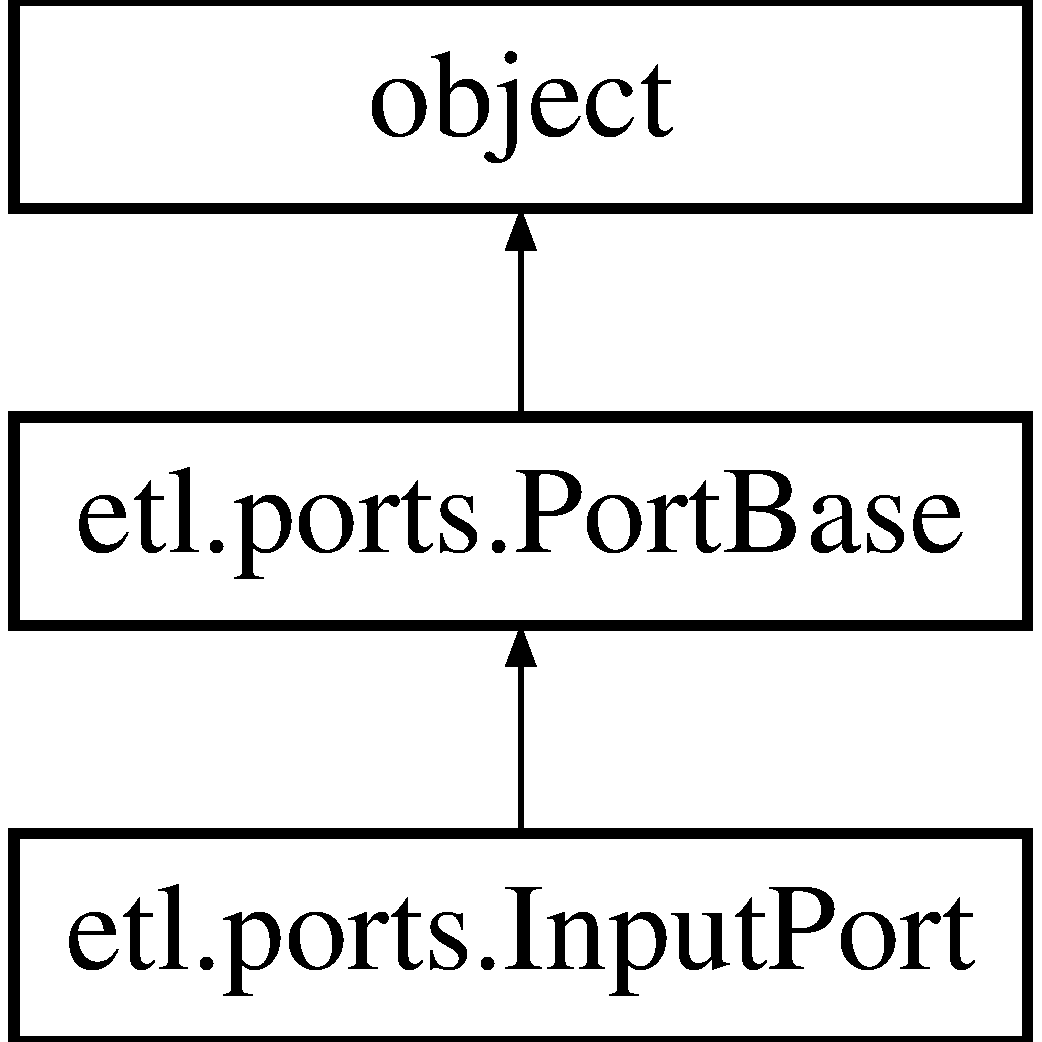
\includegraphics[height=3.000000cm]{classetl_1_1ports_1_1InputPort}
\end{center}
\end{figure}
\subsection*{Additional Inherited Members}


\subsection{Detailed Description}
\begin{DoxyVerb}Define a port that a component can recieve records on\end{DoxyVerb}
 

The documentation for this class was generated from the following file\-:\begin{DoxyCompactItemize}
\item 
src/etl/ports.\-py\end{DoxyCompactItemize}

\hypertarget{classetl_1_1ports_1_1InputPortCollection}{\section{etl.\-ports.\-Input\-Port\-Collection Class Reference}
\label{classetl_1_1ports_1_1InputPortCollection}\index{etl.\-ports.\-Input\-Port\-Collection@{etl.\-ports.\-Input\-Port\-Collection}}
}
Inheritance diagram for etl.\-ports.\-Input\-Port\-Collection\-:\begin{figure}[H]
\begin{center}
\leavevmode
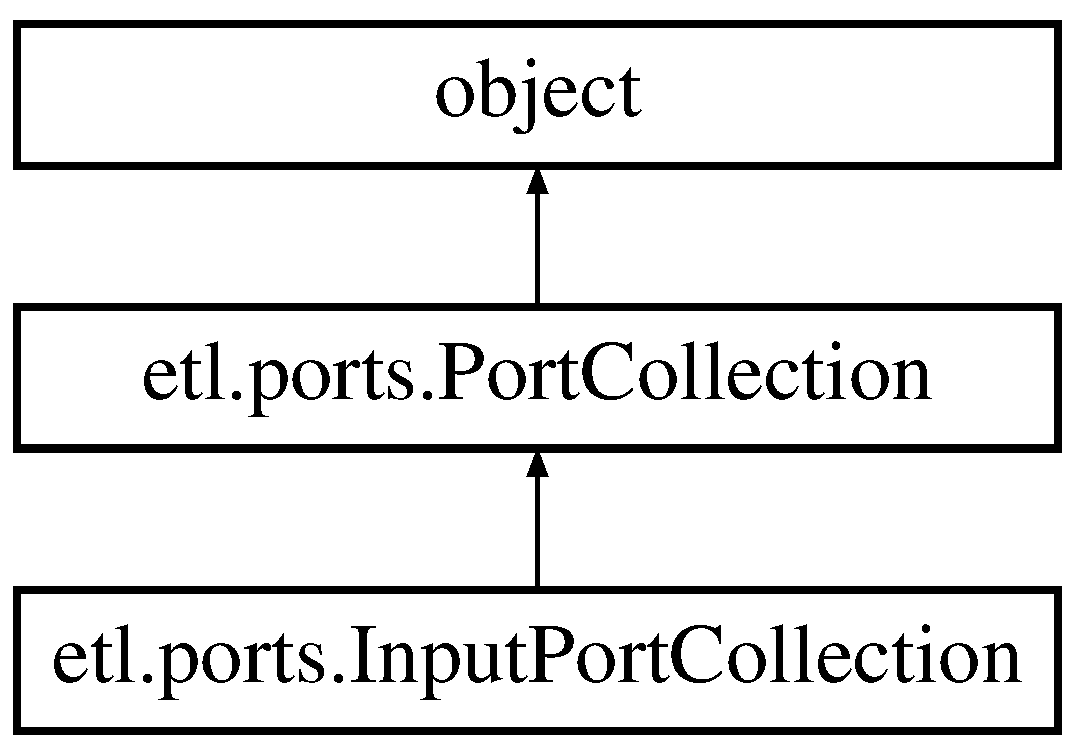
\includegraphics[height=3.000000cm]{classetl_1_1ports_1_1InputPortCollection}
\end{center}
\end{figure}
\subsection*{Public Member Functions}
\begin{DoxyCompactItemize}
\item 
def \hyperlink{classetl_1_1ports_1_1InputPortCollection_ac3683354a87d42cecf4201c842d5d00c}{\-\_\-\-\_\-init\-\_\-\-\_\-}
\end{DoxyCompactItemize}
\subsection*{Public Attributes}
\begin{DoxyCompactItemize}
\item 
\hypertarget{classetl_1_1ports_1_1InputPortCollection_af12748c8e1c9507ab18a52bd46bb8a31}{{\bfseries input\-\_\-lock}}\label{classetl_1_1ports_1_1InputPortCollection_af12748c8e1c9507ab18a52bd46bb8a31}

\end{DoxyCompactItemize}


\subsection{Detailed Description}
\begin{DoxyVerb}Collection of all input ports for a processor\end{DoxyVerb}
 

\subsection{Constructor \& Destructor Documentation}
\hypertarget{classetl_1_1ports_1_1InputPortCollection_ac3683354a87d42cecf4201c842d5d00c}{\index{etl\-::ports\-::\-Input\-Port\-Collection@{etl\-::ports\-::\-Input\-Port\-Collection}!\-\_\-\-\_\-init\-\_\-\-\_\-@{\-\_\-\-\_\-init\-\_\-\-\_\-}}
\index{\-\_\-\-\_\-init\-\_\-\-\_\-@{\-\_\-\-\_\-init\-\_\-\-\_\-}!etl::ports::InputPortCollection@{etl\-::ports\-::\-Input\-Port\-Collection}}
\subsubsection[{\-\_\-\-\_\-init\-\_\-\-\_\-}]{\setlength{\rightskip}{0pt plus 5cm}def etl.\-ports.\-Input\-Port\-Collection.\-\_\-\-\_\-init\-\_\-\-\_\- (
\begin{DoxyParamCaption}
\item[{}]{self, }
\item[{}]{name}
\end{DoxyParamCaption}
)}}\label{classetl_1_1ports_1_1InputPortCollection_ac3683354a87d42cecf4201c842d5d00c}
\begin{DoxyVerb}Collection of all input ports for a processor\end{DoxyVerb}
 

The documentation for this class was generated from the following file\-:\begin{DoxyCompactItemize}
\item 
src/etl/ports.\-py\end{DoxyCompactItemize}

\hypertarget{classetl_1_1ports_1_1OutputPort}{\section{etl.\-ports.\-Output\-Port Class Reference}
\label{classetl_1_1ports_1_1OutputPort}\index{etl.\-ports.\-Output\-Port@{etl.\-ports.\-Output\-Port}}
}
Inheritance diagram for etl.\-ports.\-Output\-Port\-:\begin{figure}[H]
\begin{center}
\leavevmode
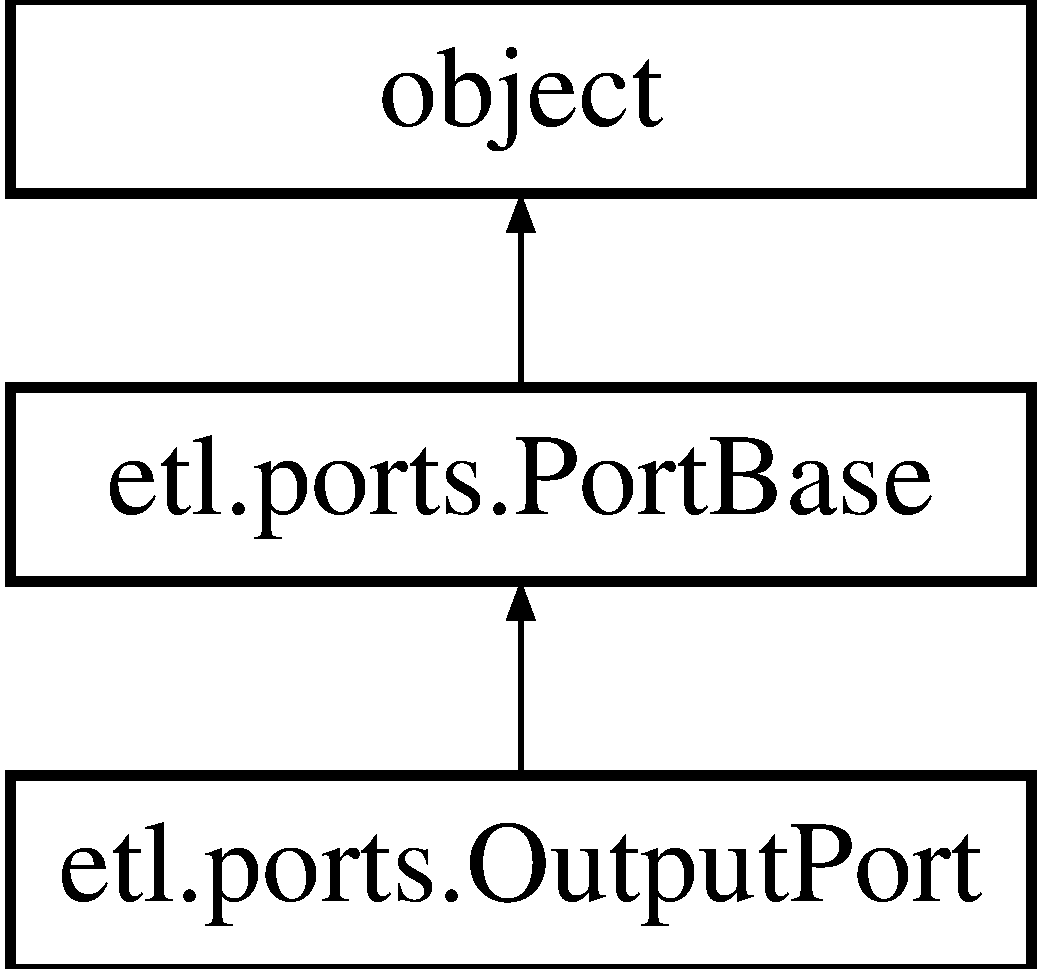
\includegraphics[height=3.000000cm]{classetl_1_1ports_1_1OutputPort}
\end{center}
\end{figure}
\subsection*{Additional Inherited Members}


\subsection{Detailed Description}
\begin{DoxyVerb}Define a port that a component can dispatch records on\end{DoxyVerb}
 

The documentation for this class was generated from the following file\-:\begin{DoxyCompactItemize}
\item 
src/etl/ports.\-py\end{DoxyCompactItemize}

\hypertarget{classetl_1_1ports_1_1OutputPortCollection}{\section{etl.\-ports.\-Output\-Port\-Collection Class Reference}
\label{classetl_1_1ports_1_1OutputPortCollection}\index{etl.\-ports.\-Output\-Port\-Collection@{etl.\-ports.\-Output\-Port\-Collection}}
}
Inheritance diagram for etl.\-ports.\-Output\-Port\-Collection\-:\begin{figure}[H]
\begin{center}
\leavevmode
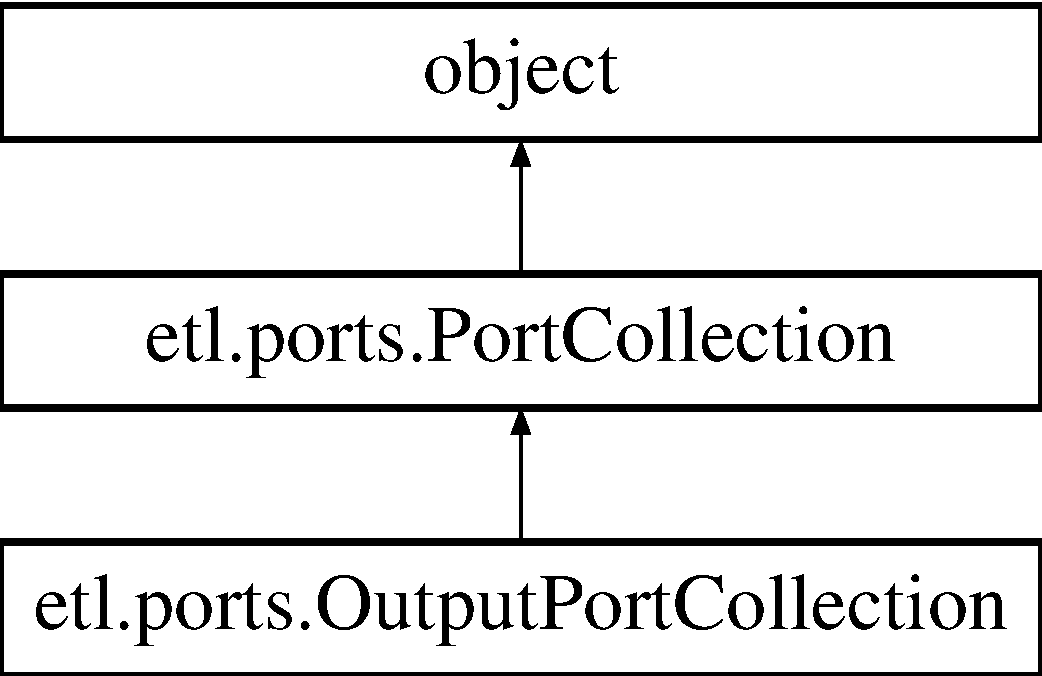
\includegraphics[height=3.000000cm]{classetl_1_1ports_1_1OutputPortCollection}
\end{center}
\end{figure}
\subsection*{Additional Inherited Members}


\subsection{Detailed Description}
\begin{DoxyVerb}Collection of all input ports for a processor\end{DoxyVerb}
 

The documentation for this class was generated from the following file\-:\begin{DoxyCompactItemize}
\item 
src/etl/ports.\-py\end{DoxyCompactItemize}

\hypertarget{classetl_1_1ports_1_1PortBase}{\section{etl.\-ports.\-Port\-Base Class Reference}
\label{classetl_1_1ports_1_1PortBase}\index{etl.\-ports.\-Port\-Base@{etl.\-ports.\-Port\-Base}}
}
Inheritance diagram for etl.\-ports.\-Port\-Base\-:\begin{figure}[H]
\begin{center}
\leavevmode
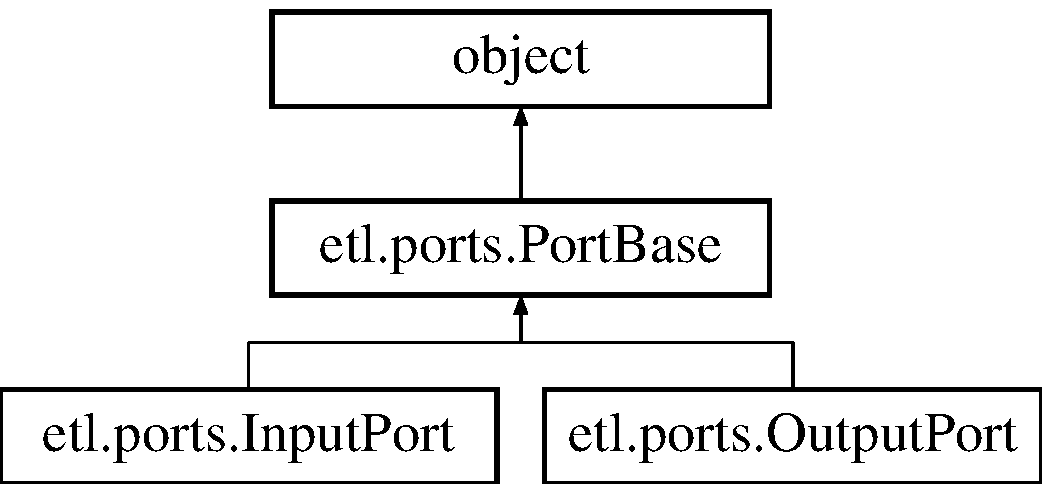
\includegraphics[height=3.000000cm]{classetl_1_1ports_1_1PortBase}
\end{center}
\end{figure}
\subsection*{Public Member Functions}
\begin{DoxyCompactItemize}
\item 
def \hyperlink{classetl_1_1ports_1_1PortBase_aff45a15ce5dfd579e777f58e282902d3}{\-\_\-\-\_\-init\-\_\-\-\_\-}
\item 
\hypertarget{classetl_1_1ports_1_1PortBase_a8e41de2b468098d33b8b8ccc83a0bbc9}{def {\bfseries name}}\label{classetl_1_1ports_1_1PortBase_a8e41de2b468098d33b8b8ccc83a0bbc9}

\end{DoxyCompactItemize}


\subsection{Detailed Description}
\begin{DoxyVerb}Base class for InputPortCollection and OutputPortCollection\end{DoxyVerb}
 

\subsection{Constructor \& Destructor Documentation}
\hypertarget{classetl_1_1ports_1_1PortBase_aff45a15ce5dfd579e777f58e282902d3}{\index{etl\-::ports\-::\-Port\-Base@{etl\-::ports\-::\-Port\-Base}!\-\_\-\-\_\-init\-\_\-\-\_\-@{\-\_\-\-\_\-init\-\_\-\-\_\-}}
\index{\-\_\-\-\_\-init\-\_\-\-\_\-@{\-\_\-\-\_\-init\-\_\-\-\_\-}!etl::ports::PortBase@{etl\-::ports\-::\-Port\-Base}}
\subsubsection[{\-\_\-\-\_\-init\-\_\-\-\_\-}]{\setlength{\rightskip}{0pt plus 5cm}def etl.\-ports.\-Port\-Base.\-\_\-\-\_\-init\-\_\-\-\_\- (
\begin{DoxyParamCaption}
\item[{}]{self, }
\item[{}]{name}
\end{DoxyParamCaption}
)}}\label{classetl_1_1ports_1_1PortBase_aff45a15ce5dfd579e777f58e282902d3}
\begin{DoxyVerb}Init 

@param name: Name of the port for forming connections
\end{DoxyVerb}
 

The documentation for this class was generated from the following file\-:\begin{DoxyCompactItemize}
\item 
src/etl/ports.\-py\end{DoxyCompactItemize}

\hypertarget{classetl_1_1ports_1_1PortCollection}{\section{etl.\-ports.\-Port\-Collection Class Reference}
\label{classetl_1_1ports_1_1PortCollection}\index{etl.\-ports.\-Port\-Collection@{etl.\-ports.\-Port\-Collection}}
}
Inheritance diagram for etl.\-ports.\-Port\-Collection\-:\begin{figure}[H]
\begin{center}
\leavevmode
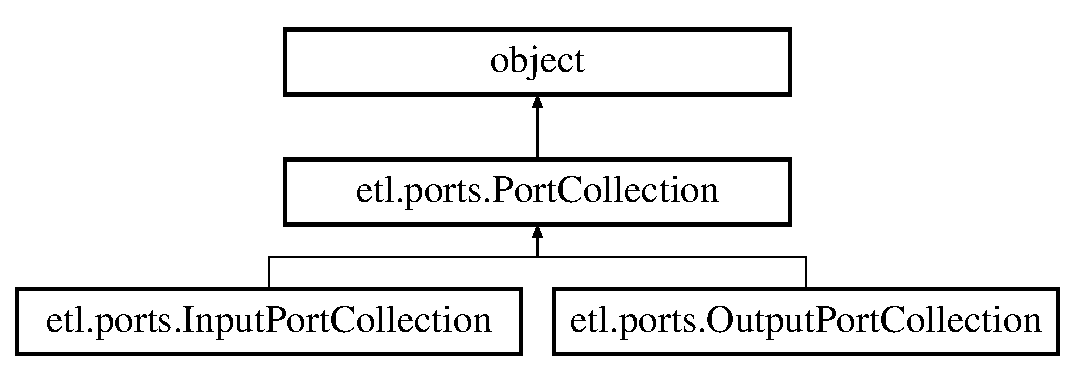
\includegraphics[height=3.000000cm]{classetl_1_1ports_1_1PortCollection}
\end{center}
\end{figure}
\subsection*{Public Member Functions}
\begin{DoxyCompactItemize}
\item 
\hypertarget{classetl_1_1ports_1_1PortCollection_a5e99222968dfd477ff7fec16c1173d53}{def {\bfseries \-\_\-\-\_\-init\-\_\-\-\_\-}}\label{classetl_1_1ports_1_1PortCollection_a5e99222968dfd477ff7fec16c1173d53}

\item 
def \hyperlink{classetl_1_1ports_1_1PortCollection_ae7352bbb10c54f38333ef1a06581dfcc}{create\-\_\-port}
\end{DoxyCompactItemize}


\subsection{Detailed Description}
\begin{DoxyVerb}Base class for InputPorts and OutputPorts\end{DoxyVerb}
 

\subsection{Member Function Documentation}
\hypertarget{classetl_1_1ports_1_1PortCollection_ae7352bbb10c54f38333ef1a06581dfcc}{\index{etl\-::ports\-::\-Port\-Collection@{etl\-::ports\-::\-Port\-Collection}!create\-\_\-port@{create\-\_\-port}}
\index{create\-\_\-port@{create\-\_\-port}!etl::ports::PortCollection@{etl\-::ports\-::\-Port\-Collection}}
\subsubsection[{create\-\_\-port}]{\setlength{\rightskip}{0pt plus 5cm}def etl.\-ports.\-Port\-Collection.\-create\-\_\-port (
\begin{DoxyParamCaption}
\item[{}]{self, }
\item[{}]{name}
\end{DoxyParamCaption}
)}}\label{classetl_1_1ports_1_1PortCollection_ae7352bbb10c54f38333ef1a06581dfcc}
\begin{DoxyVerb}Define a new port\end{DoxyVerb}
 

The documentation for this class was generated from the following file\-:\begin{DoxyCompactItemize}
\item 
src/etl/ports.\-py\end{DoxyCompactItemize}

\hypertarget{classetl_1_1PostRecordProcessingAction_1_1GetNextInputRecord}{\section{etl.\-Post\-Record\-Processing\-Action.\-Get\-Next\-Input\-Record Class Reference}
\label{classetl_1_1PostRecordProcessingAction_1_1GetNextInputRecord}\index{etl.\-Post\-Record\-Processing\-Action.\-Get\-Next\-Input\-Record@{etl.\-Post\-Record\-Processing\-Action.\-Get\-Next\-Input\-Record}}
}
Inheritance diagram for etl.\-Post\-Record\-Processing\-Action.\-Get\-Next\-Input\-Record\-:\begin{figure}[H]
\begin{center}
\leavevmode
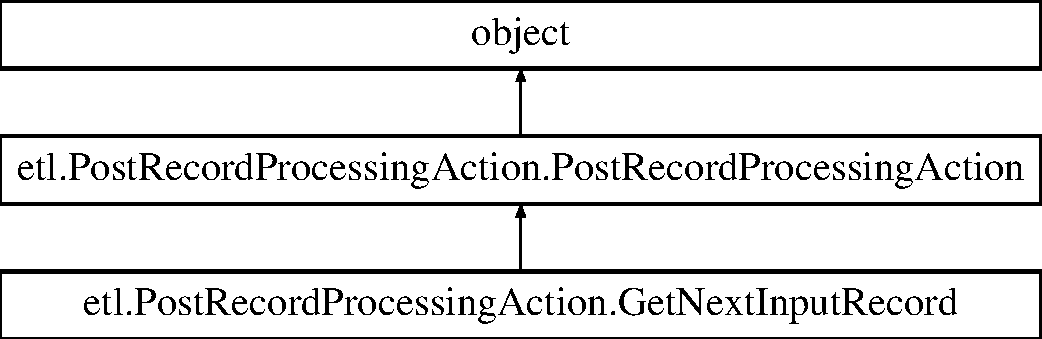
\includegraphics[height=3.000000cm]{classetl_1_1PostRecordProcessingAction_1_1GetNextInputRecord}
\end{center}
\end{figure}
\subsection*{Public Member Functions}
\begin{DoxyCompactItemize}
\item 
\hypertarget{classetl_1_1PostRecordProcessingAction_1_1GetNextInputRecord_a2de2ecd67e4bf4767686ce90ed80d3e5}{def {\bfseries \-\_\-\-\_\-init\-\_\-\-\_\-}}\label{classetl_1_1PostRecordProcessingAction_1_1GetNextInputRecord_a2de2ecd67e4bf4767686ce90ed80d3e5}

\end{DoxyCompactItemize}
\subsection*{Public Attributes}
\begin{DoxyCompactItemize}
\item 
\hypertarget{classetl_1_1PostRecordProcessingAction_1_1GetNextInputRecord_ab591c1210614fb122bbca0ccdf2e4815}{{\bfseries input\-\_\-name}}\label{classetl_1_1PostRecordProcessingAction_1_1GetNextInputRecord_ab591c1210614fb122bbca0ccdf2e4815}

\end{DoxyCompactItemize}


\subsection{Detailed Description}
\begin{DoxyVerb}Instruct processor to immediately retrieve the next buffered record

This grabs the next record on the specified input and calls
prc_input_record() again without processing additional events on the event
queue first.  This is typically used to process through previously held
(HoldRecord) records.  If no additional records exist on the specified
input, then processor will continue processing the event queue.

This response implies RecordConsumed, and the record passed in to
prc_input_record() will be popped off the incoming queue.
\end{DoxyVerb}
 

The documentation for this class was generated from the following file\-:\begin{DoxyCompactItemize}
\item 
src/etl/Post\-Record\-Processing\-Action.\-py\end{DoxyCompactItemize}

\hypertarget{classetl_1_1PostRecordProcessingAction_1_1HoldRecord}{\section{etl.\-Post\-Record\-Processing\-Action.\-Hold\-Record Class Reference}
\label{classetl_1_1PostRecordProcessingAction_1_1HoldRecord}\index{etl.\-Post\-Record\-Processing\-Action.\-Hold\-Record@{etl.\-Post\-Record\-Processing\-Action.\-Hold\-Record}}
}
Inheritance diagram for etl.\-Post\-Record\-Processing\-Action.\-Hold\-Record\-:\begin{figure}[H]
\begin{center}
\leavevmode
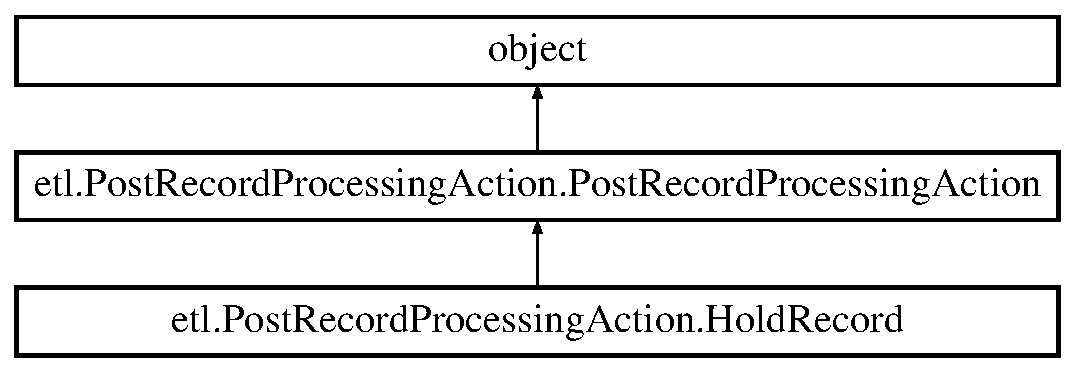
\includegraphics[height=3.000000cm]{classetl_1_1PostRecordProcessingAction_1_1HoldRecord}
\end{center}
\end{figure}
\subsection*{Public Member Functions}
\begin{DoxyCompactItemize}
\item 
\hypertarget{classetl_1_1PostRecordProcessingAction_1_1HoldRecord_aa336212ee73ea5ed34317910e313b512}{def {\bfseries \-\_\-\-\_\-init\-\_\-\-\_\-}}\label{classetl_1_1PostRecordProcessingAction_1_1HoldRecord_aa336212ee73ea5ed34317910e313b512}

\end{DoxyCompactItemize}


\subsection{Detailed Description}
\begin{DoxyVerb}Instruct processor that record has not been processed yet.

This holds the record on the input queue until GetNextInputRecord is
called
\end{DoxyVerb}
 

The documentation for this class was generated from the following file\-:\begin{DoxyCompactItemize}
\item 
src/etl/Post\-Record\-Processing\-Action.\-py\end{DoxyCompactItemize}

\hypertarget{classetl_1_1PostRecordProcessingAction_1_1PostRecordProcessingAction}{\section{etl.\-Post\-Record\-Processing\-Action.\-Post\-Record\-Processing\-Action Class Reference}
\label{classetl_1_1PostRecordProcessingAction_1_1PostRecordProcessingAction}\index{etl.\-Post\-Record\-Processing\-Action.\-Post\-Record\-Processing\-Action@{etl.\-Post\-Record\-Processing\-Action.\-Post\-Record\-Processing\-Action}}
}
Inheritance diagram for etl.\-Post\-Record\-Processing\-Action.\-Post\-Record\-Processing\-Action\-:\begin{figure}[H]
\begin{center}
\leavevmode
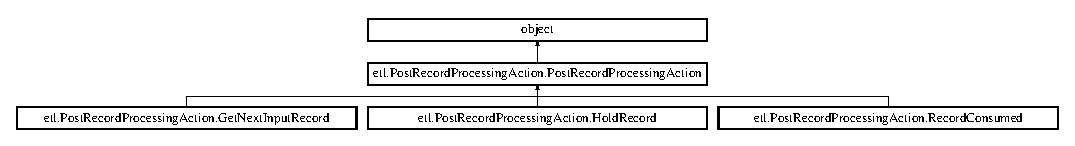
\includegraphics[height=1.517615cm]{classetl_1_1PostRecordProcessingAction_1_1PostRecordProcessingAction}
\end{center}
\end{figure}
\subsection*{Public Member Functions}
\begin{DoxyCompactItemize}
\item 
\hypertarget{classetl_1_1PostRecordProcessingAction_1_1PostRecordProcessingAction_a28bbda2ee13e5c1adb09a2af2cb0a401}{def {\bfseries \-\_\-\-\_\-init\-\_\-\-\_\-}}\label{classetl_1_1PostRecordProcessingAction_1_1PostRecordProcessingAction_a28bbda2ee13e5c1adb09a2af2cb0a401}

\item 
\hypertarget{classetl_1_1PostRecordProcessingAction_1_1PostRecordProcessingAction_a08cc167e5e4c084a80b2133542e0f66b}{def {\bfseries code}}\label{classetl_1_1PostRecordProcessingAction_1_1PostRecordProcessingAction_a08cc167e5e4c084a80b2133542e0f66b}

\end{DoxyCompactItemize}


\subsection{Detailed Description}
\begin{DoxyVerb}Action to take after a record is processed by prc_input_record()

This instructs the Processors Event on what to do with the input record
that was just processed.  This is provided primarily to allow a processor
to declare that it did not process an input record, and will request it
later
\end{DoxyVerb}
 

The documentation for this class was generated from the following file\-:\begin{DoxyCompactItemize}
\item 
src/etl/Post\-Record\-Processing\-Action.\-py\end{DoxyCompactItemize}

\hypertarget{classetl_1_1PostRecordProcessingAction_1_1RecordConsumed}{\section{etl.\-Post\-Record\-Processing\-Action.\-Record\-Consumed Class Reference}
\label{classetl_1_1PostRecordProcessingAction_1_1RecordConsumed}\index{etl.\-Post\-Record\-Processing\-Action.\-Record\-Consumed@{etl.\-Post\-Record\-Processing\-Action.\-Record\-Consumed}}
}
Inheritance diagram for etl.\-Post\-Record\-Processing\-Action.\-Record\-Consumed\-:\begin{figure}[H]
\begin{center}
\leavevmode
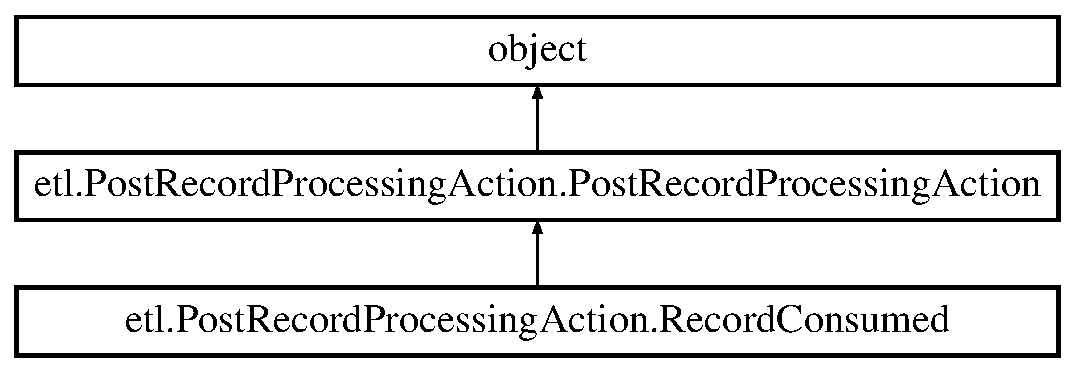
\includegraphics[height=3.000000cm]{classetl_1_1PostRecordProcessingAction_1_1RecordConsumed}
\end{center}
\end{figure}
\subsection*{Public Member Functions}
\begin{DoxyCompactItemize}
\item 
\hypertarget{classetl_1_1PostRecordProcessingAction_1_1RecordConsumed_abcb6479d91dff3ce5f739714abd7e12e}{def {\bfseries \-\_\-\-\_\-init\-\_\-\-\_\-}}\label{classetl_1_1PostRecordProcessingAction_1_1RecordConsumed_abcb6479d91dff3ce5f739714abd7e12e}

\end{DoxyCompactItemize}


\subsection{Detailed Description}
\begin{DoxyVerb}Signify that the record was processed, and can be discarded.

This is the default assumed action if None is returned from
prc_input_record()
\end{DoxyVerb}
 

The documentation for this class was generated from the following file\-:\begin{DoxyCompactItemize}
\item 
src/etl/Post\-Record\-Processing\-Action.\-py\end{DoxyCompactItemize}

\hypertarget{classetl_1_1recshelf_1_1MemoryRecordSet_1_1MemoryRecordSet}{\section{etl.\-recshelf.\-Memory\-Record\-Set.\-Memory\-Record\-Set Class Reference}
\label{classetl_1_1recshelf_1_1MemoryRecordSet_1_1MemoryRecordSet}\index{etl.\-recshelf.\-Memory\-Record\-Set.\-Memory\-Record\-Set@{etl.\-recshelf.\-Memory\-Record\-Set.\-Memory\-Record\-Set}}
}
Inheritance diagram for etl.\-recshelf.\-Memory\-Record\-Set.\-Memory\-Record\-Set\-:\begin{figure}[H]
\begin{center}
\leavevmode
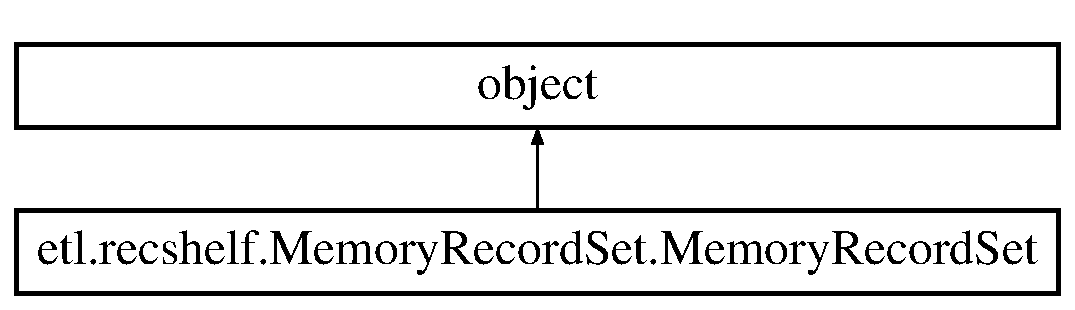
\includegraphics[height=2.000000cm]{classetl_1_1recshelf_1_1MemoryRecordSet_1_1MemoryRecordSet}
\end{center}
\end{figure}
\subsection*{Public Member Functions}
\begin{DoxyCompactItemize}
\item 
\hypertarget{classetl_1_1recshelf_1_1MemoryRecordSet_1_1MemoryRecordSet_ad19e823f909c56fcda06829b2aa4208a}{def {\bfseries \-\_\-\-\_\-init\-\_\-\-\_\-}}\label{classetl_1_1recshelf_1_1MemoryRecordSet_1_1MemoryRecordSet_ad19e823f909c56fcda06829b2aa4208a}

\item 
def \hyperlink{classetl_1_1recshelf_1_1MemoryRecordSet_1_1MemoryRecordSet_afd7320b379c5c7e045f2616252337fc6}{dump\-\_\-records}
\item 
def \hyperlink{classetl_1_1recshelf_1_1MemoryRecordSet_1_1MemoryRecordSet_a00d61494917b21379a954d9ce997ca31}{add\-\_\-record}
\item 
def \hyperlink{classetl_1_1recshelf_1_1MemoryRecordSet_1_1MemoryRecordSet_a6c655eb1e6cfb73a9516c165fbb5c682}{get\-\_\-record}
\item 
\hypertarget{classetl_1_1recshelf_1_1MemoryRecordSet_1_1MemoryRecordSet_aa138fc96e0100b2e800bfa415c2b9d3e}{def {\bfseries has\-\_\-record}}\label{classetl_1_1recshelf_1_1MemoryRecordSet_1_1MemoryRecordSet_aa138fc96e0100b2e800bfa415c2b9d3e}

\item 
def \hyperlink{classetl_1_1recshelf_1_1MemoryRecordSet_1_1MemoryRecordSet_aad7c550515b18387e7b2c3df06447ea2}{find\-\_\-records\-\_\-with\-\_\-tag}
\item 
\hypertarget{classetl_1_1recshelf_1_1MemoryRecordSet_1_1MemoryRecordSet_a8d7c09c79fc751c7a84c40ba73f91888}{def {\bfseries has\-\_\-record\-\_\-with\-\_\-tag}}\label{classetl_1_1recshelf_1_1MemoryRecordSet_1_1MemoryRecordSet_a8d7c09c79fc751c7a84c40ba73f91888}

\item 
def \hyperlink{classetl_1_1recshelf_1_1MemoryRecordSet_1_1MemoryRecordSet_a6b8f6fa6dba066f9f1ee9bb52dcf7568}{remove\-\_\-record}
\item 
def \hyperlink{classetl_1_1recshelf_1_1MemoryRecordSet_1_1MemoryRecordSet_a9bb4a7678b7a8f7bcd7d46ea9ab789aa}{size}
\item 
\hypertarget{classetl_1_1recshelf_1_1MemoryRecordSet_1_1MemoryRecordSet_a7d8f79931efa62a7ea2598668506acce}{def {\bfseries count}}\label{classetl_1_1recshelf_1_1MemoryRecordSet_1_1MemoryRecordSet_a7d8f79931efa62a7ea2598668506acce}

\end{DoxyCompactItemize}


\subsection{Detailed Description}
\begin{DoxyVerb}Stores records in memory.

Don't use this class directly, but use EtlRecordSet instead
\end{DoxyVerb}
 

\subsection{Member Function Documentation}
\hypertarget{classetl_1_1recshelf_1_1MemoryRecordSet_1_1MemoryRecordSet_a00d61494917b21379a954d9ce997ca31}{\index{etl\-::recshelf\-::\-Memory\-Record\-Set\-::\-Memory\-Record\-Set@{etl\-::recshelf\-::\-Memory\-Record\-Set\-::\-Memory\-Record\-Set}!add\-\_\-record@{add\-\_\-record}}
\index{add\-\_\-record@{add\-\_\-record}!etl::recshelf::MemoryRecordSet::MemoryRecordSet@{etl\-::recshelf\-::\-Memory\-Record\-Set\-::\-Memory\-Record\-Set}}
\subsubsection[{add\-\_\-record}]{\setlength{\rightskip}{0pt plus 5cm}def etl.\-recshelf.\-Memory\-Record\-Set.\-Memory\-Record\-Set.\-add\-\_\-record (
\begin{DoxyParamCaption}
\item[{}]{self, }
\item[{}]{etl\-\_\-rec, }
\item[{}]{tags = {\ttfamily None}}
\end{DoxyParamCaption}
)}}\label{classetl_1_1recshelf_1_1MemoryRecordSet_1_1MemoryRecordSet_a00d61494917b21379a954d9ce997ca31}
\begin{DoxyVerb}Add a record to the collection

Use indexes to index this 

@param etl_rec: Record to store
@param tags: List of optional additional tags to be used for retrieving
    this record.  Record must be convertable to a string with str()
\end{DoxyVerb}
 \hypertarget{classetl_1_1recshelf_1_1MemoryRecordSet_1_1MemoryRecordSet_afd7320b379c5c7e045f2616252337fc6}{\index{etl\-::recshelf\-::\-Memory\-Record\-Set\-::\-Memory\-Record\-Set@{etl\-::recshelf\-::\-Memory\-Record\-Set\-::\-Memory\-Record\-Set}!dump\-\_\-records@{dump\-\_\-records}}
\index{dump\-\_\-records@{dump\-\_\-records}!etl::recshelf::MemoryRecordSet::MemoryRecordSet@{etl\-::recshelf\-::\-Memory\-Record\-Set\-::\-Memory\-Record\-Set}}
\subsubsection[{dump\-\_\-records}]{\setlength{\rightskip}{0pt plus 5cm}def etl.\-recshelf.\-Memory\-Record\-Set.\-Memory\-Record\-Set.\-dump\-\_\-records (
\begin{DoxyParamCaption}
\item[{}]{self}
\end{DoxyParamCaption}
)}}\label{classetl_1_1recshelf_1_1MemoryRecordSet_1_1MemoryRecordSet_afd7320b379c5c7e045f2616252337fc6}
\begin{DoxyVerb}Return all records

@return: Generator of (record, tags)
\end{DoxyVerb}
 \hypertarget{classetl_1_1recshelf_1_1MemoryRecordSet_1_1MemoryRecordSet_aad7c550515b18387e7b2c3df06447ea2}{\index{etl\-::recshelf\-::\-Memory\-Record\-Set\-::\-Memory\-Record\-Set@{etl\-::recshelf\-::\-Memory\-Record\-Set\-::\-Memory\-Record\-Set}!find\-\_\-records\-\_\-with\-\_\-tag@{find\-\_\-records\-\_\-with\-\_\-tag}}
\index{find\-\_\-records\-\_\-with\-\_\-tag@{find\-\_\-records\-\_\-with\-\_\-tag}!etl::recshelf::MemoryRecordSet::MemoryRecordSet@{etl\-::recshelf\-::\-Memory\-Record\-Set\-::\-Memory\-Record\-Set}}
\subsubsection[{find\-\_\-records\-\_\-with\-\_\-tag}]{\setlength{\rightskip}{0pt plus 5cm}def etl.\-recshelf.\-Memory\-Record\-Set.\-Memory\-Record\-Set.\-find\-\_\-records\-\_\-with\-\_\-tag (
\begin{DoxyParamCaption}
\item[{}]{self, }
\item[{}]{tag}
\end{DoxyParamCaption}
)}}\label{classetl_1_1recshelf_1_1MemoryRecordSet_1_1MemoryRecordSet_aad7c550515b18387e7b2c3df06447ea2}
\begin{DoxyVerb}Find records that have a given tag\end{DoxyVerb}
 \hypertarget{classetl_1_1recshelf_1_1MemoryRecordSet_1_1MemoryRecordSet_a6c655eb1e6cfb73a9516c165fbb5c682}{\index{etl\-::recshelf\-::\-Memory\-Record\-Set\-::\-Memory\-Record\-Set@{etl\-::recshelf\-::\-Memory\-Record\-Set\-::\-Memory\-Record\-Set}!get\-\_\-record@{get\-\_\-record}}
\index{get\-\_\-record@{get\-\_\-record}!etl::recshelf::MemoryRecordSet::MemoryRecordSet@{etl\-::recshelf\-::\-Memory\-Record\-Set\-::\-Memory\-Record\-Set}}
\subsubsection[{get\-\_\-record}]{\setlength{\rightskip}{0pt plus 5cm}def etl.\-recshelf.\-Memory\-Record\-Set.\-Memory\-Record\-Set.\-get\-\_\-record (
\begin{DoxyParamCaption}
\item[{}]{self, }
\item[{}]{serial}
\end{DoxyParamCaption}
)}}\label{classetl_1_1recshelf_1_1MemoryRecordSet_1_1MemoryRecordSet_a6c655eb1e6cfb73a9516c165fbb5c682}
\begin{DoxyVerb}Retrieve a record

@param serical:
    Record identifier
@return EtlRecord
\end{DoxyVerb}
 \hypertarget{classetl_1_1recshelf_1_1MemoryRecordSet_1_1MemoryRecordSet_a6b8f6fa6dba066f9f1ee9bb52dcf7568}{\index{etl\-::recshelf\-::\-Memory\-Record\-Set\-::\-Memory\-Record\-Set@{etl\-::recshelf\-::\-Memory\-Record\-Set\-::\-Memory\-Record\-Set}!remove\-\_\-record@{remove\-\_\-record}}
\index{remove\-\_\-record@{remove\-\_\-record}!etl::recshelf::MemoryRecordSet::MemoryRecordSet@{etl\-::recshelf\-::\-Memory\-Record\-Set\-::\-Memory\-Record\-Set}}
\subsubsection[{remove\-\_\-record}]{\setlength{\rightskip}{0pt plus 5cm}def etl.\-recshelf.\-Memory\-Record\-Set.\-Memory\-Record\-Set.\-remove\-\_\-record (
\begin{DoxyParamCaption}
\item[{}]{self, }
\item[{}]{serial}
\end{DoxyParamCaption}
)}}\label{classetl_1_1recshelf_1_1MemoryRecordSet_1_1MemoryRecordSet_a6b8f6fa6dba066f9f1ee9bb52dcf7568}
\begin{DoxyVerb}Drop a record from the collection\end{DoxyVerb}
 \hypertarget{classetl_1_1recshelf_1_1MemoryRecordSet_1_1MemoryRecordSet_a9bb4a7678b7a8f7bcd7d46ea9ab789aa}{\index{etl\-::recshelf\-::\-Memory\-Record\-Set\-::\-Memory\-Record\-Set@{etl\-::recshelf\-::\-Memory\-Record\-Set\-::\-Memory\-Record\-Set}!size@{size}}
\index{size@{size}!etl::recshelf::MemoryRecordSet::MemoryRecordSet@{etl\-::recshelf\-::\-Memory\-Record\-Set\-::\-Memory\-Record\-Set}}
\subsubsection[{size}]{\setlength{\rightskip}{0pt plus 5cm}def etl.\-recshelf.\-Memory\-Record\-Set.\-Memory\-Record\-Set.\-size (
\begin{DoxyParamCaption}
\item[{}]{self}
\end{DoxyParamCaption}
)}}\label{classetl_1_1recshelf_1_1MemoryRecordSet_1_1MemoryRecordSet_a9bb4a7678b7a8f7bcd7d46ea9ab789aa}
\begin{DoxyVerb}Estimated size of the record set\end{DoxyVerb}
 

The documentation for this class was generated from the following file\-:\begin{DoxyCompactItemize}
\item 
src/etl/recshelf/Memory\-Record\-Set.\-py\end{DoxyCompactItemize}

\hypertarget{classetl_1_1recshelf_1_1RecordShelf_1_1RecordShelf}{\section{etl.\-recshelf.\-Record\-Shelf.\-Record\-Shelf Class Reference}
\label{classetl_1_1recshelf_1_1RecordShelf_1_1RecordShelf}\index{etl.\-recshelf.\-Record\-Shelf.\-Record\-Shelf@{etl.\-recshelf.\-Record\-Shelf.\-Record\-Shelf}}
}
Inheritance diagram for etl.\-recshelf.\-Record\-Shelf.\-Record\-Shelf\-:\begin{figure}[H]
\begin{center}
\leavevmode
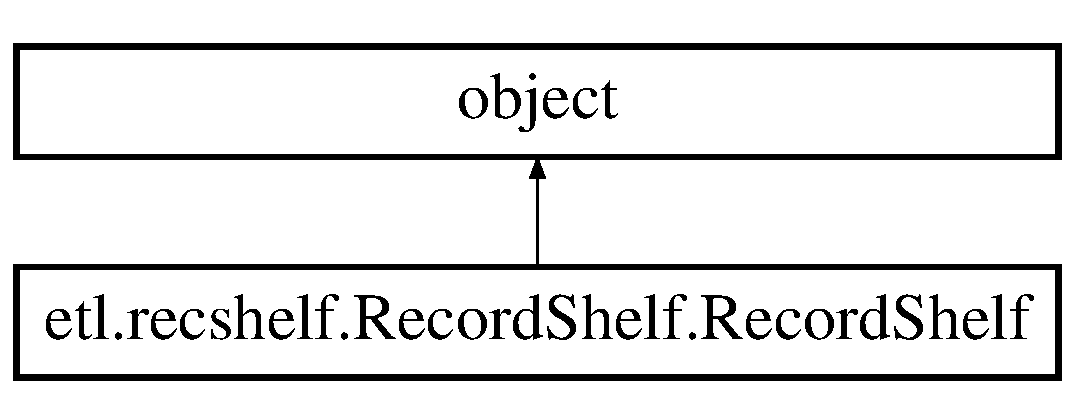
\includegraphics[height=2.000000cm]{classetl_1_1recshelf_1_1RecordShelf_1_1RecordShelf}
\end{center}
\end{figure}


\subsection{Detailed Description}
\begin{DoxyVerb}Class for storing records temporarilly\end{DoxyVerb}
 

The documentation for this class was generated from the following file\-:\begin{DoxyCompactItemize}
\item 
src/etl/recshelf/Record\-Shelf.\-py\end{DoxyCompactItemize}

\hypertarget{classetl_1_1recshelf_1_1Sqlite3RecordSet_1_1Sqlite3RecordSet}{\section{etl.\-recshelf.\-Sqlite3\-Record\-Set.\-Sqlite3\-Record\-Set Class Reference}
\label{classetl_1_1recshelf_1_1Sqlite3RecordSet_1_1Sqlite3RecordSet}\index{etl.\-recshelf.\-Sqlite3\-Record\-Set.\-Sqlite3\-Record\-Set@{etl.\-recshelf.\-Sqlite3\-Record\-Set.\-Sqlite3\-Record\-Set}}
}
Inheritance diagram for etl.\-recshelf.\-Sqlite3\-Record\-Set.\-Sqlite3\-Record\-Set\-:\begin{figure}[H]
\begin{center}
\leavevmode
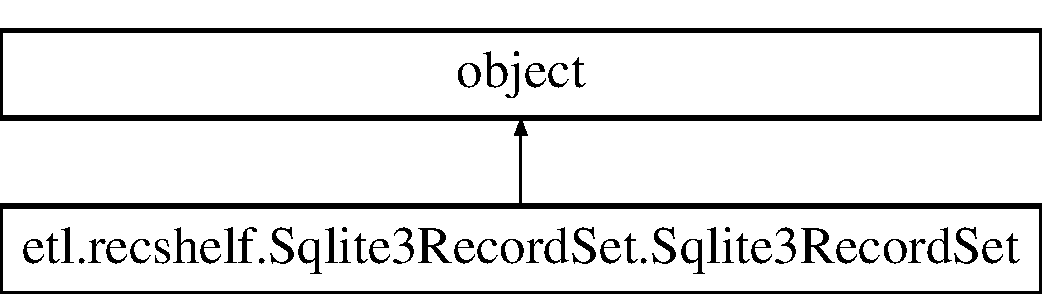
\includegraphics[height=2.000000cm]{classetl_1_1recshelf_1_1Sqlite3RecordSet_1_1Sqlite3RecordSet}
\end{center}
\end{figure}
\subsection*{Public Member Functions}
\begin{DoxyCompactItemize}
\item 
\hypertarget{classetl_1_1recshelf_1_1Sqlite3RecordSet_1_1Sqlite3RecordSet_a099ba80a1dbdc080705b2ec1820ce94c}{def {\bfseries \-\_\-\-\_\-init\-\_\-\-\_\-}}\label{classetl_1_1recshelf_1_1Sqlite3RecordSet_1_1Sqlite3RecordSet_a099ba80a1dbdc080705b2ec1820ce94c}

\item 
\hypertarget{classetl_1_1recshelf_1_1Sqlite3RecordSet_1_1Sqlite3RecordSet_a2b57962f87523d83929aa62ad1767e7c}{def {\bfseries \-\_\-\-\_\-del\-\_\-\-\_\-}}\label{classetl_1_1recshelf_1_1Sqlite3RecordSet_1_1Sqlite3RecordSet_a2b57962f87523d83929aa62ad1767e7c}

\item 
def \hyperlink{classetl_1_1recshelf_1_1Sqlite3RecordSet_1_1Sqlite3RecordSet_ad65d09d9b3b89382b61c0e9ec6890303}{add\-\_\-record}
\item 
def \hyperlink{classetl_1_1recshelf_1_1Sqlite3RecordSet_1_1Sqlite3RecordSet_ae75015047c292fc00cefbe1cf8da8f3e}{get\-\_\-record}
\item 
\hypertarget{classetl_1_1recshelf_1_1Sqlite3RecordSet_1_1Sqlite3RecordSet_a8f30e075e504b8d070047f7335d0af57}{def {\bfseries has\-\_\-record}}\label{classetl_1_1recshelf_1_1Sqlite3RecordSet_1_1Sqlite3RecordSet_a8f30e075e504b8d070047f7335d0af57}

\item 
def \hyperlink{classetl_1_1recshelf_1_1Sqlite3RecordSet_1_1Sqlite3RecordSet_aa516ec227974651d95e063e967f602c5}{find\-\_\-records\-\_\-with\-\_\-tag}
\item 
\hypertarget{classetl_1_1recshelf_1_1Sqlite3RecordSet_1_1Sqlite3RecordSet_a794132a2c4164501656630cddec3199b}{def {\bfseries has\-\_\-record\-\_\-with\-\_\-tag}}\label{classetl_1_1recshelf_1_1Sqlite3RecordSet_1_1Sqlite3RecordSet_a794132a2c4164501656630cddec3199b}

\item 
def \hyperlink{classetl_1_1recshelf_1_1Sqlite3RecordSet_1_1Sqlite3RecordSet_a0d3e7f727583a4b243e1266d5ef9c53e}{remove\-\_\-record}
\item 
def \hyperlink{classetl_1_1recshelf_1_1Sqlite3RecordSet_1_1Sqlite3RecordSet_ad802dc96c74be57424e97c78bef89395}{size}
\item 
\hypertarget{classetl_1_1recshelf_1_1Sqlite3RecordSet_1_1Sqlite3RecordSet_a60446a028ff878f6720b2cded88bd11e}{def {\bfseries count}}\label{classetl_1_1recshelf_1_1Sqlite3RecordSet_1_1Sqlite3RecordSet_a60446a028ff878f6720b2cded88bd11e}

\item 
\hypertarget{classetl_1_1recshelf_1_1Sqlite3RecordSet_1_1Sqlite3RecordSet_a19b8d14b17d9d08d47f52b605d96f8e3}{def {\bfseries db\-\_\-path}}\label{classetl_1_1recshelf_1_1Sqlite3RecordSet_1_1Sqlite3RecordSet_a19b8d14b17d9d08d47f52b605d96f8e3}

\end{DoxyCompactItemize}


\subsection{Detailed Description}
\begin{DoxyVerb}Stores records into an sqlite3 database.

Don't use this class directly, but use EtlRecordSet instead
\end{DoxyVerb}
 

\subsection{Member Function Documentation}
\hypertarget{classetl_1_1recshelf_1_1Sqlite3RecordSet_1_1Sqlite3RecordSet_ad65d09d9b3b89382b61c0e9ec6890303}{\index{etl\-::recshelf\-::\-Sqlite3\-Record\-Set\-::\-Sqlite3\-Record\-Set@{etl\-::recshelf\-::\-Sqlite3\-Record\-Set\-::\-Sqlite3\-Record\-Set}!add\-\_\-record@{add\-\_\-record}}
\index{add\-\_\-record@{add\-\_\-record}!etl::recshelf::Sqlite3RecordSet::Sqlite3RecordSet@{etl\-::recshelf\-::\-Sqlite3\-Record\-Set\-::\-Sqlite3\-Record\-Set}}
\subsubsection[{add\-\_\-record}]{\setlength{\rightskip}{0pt plus 5cm}def etl.\-recshelf.\-Sqlite3\-Record\-Set.\-Sqlite3\-Record\-Set.\-add\-\_\-record (
\begin{DoxyParamCaption}
\item[{}]{self, }
\item[{}]{etl\-\_\-rec, }
\item[{}]{tags = {\ttfamily None}}
\end{DoxyParamCaption}
)}}\label{classetl_1_1recshelf_1_1Sqlite3RecordSet_1_1Sqlite3RecordSet_ad65d09d9b3b89382b61c0e9ec6890303}
\begin{DoxyVerb}Add a record to the collection

Use indexes to index this 

@param etl_rec: Record to store
@param tags: List of optional additional tags to be used for retrieving
    this record.  Record must be convertable to a string with str()
\end{DoxyVerb}
 \hypertarget{classetl_1_1recshelf_1_1Sqlite3RecordSet_1_1Sqlite3RecordSet_aa516ec227974651d95e063e967f602c5}{\index{etl\-::recshelf\-::\-Sqlite3\-Record\-Set\-::\-Sqlite3\-Record\-Set@{etl\-::recshelf\-::\-Sqlite3\-Record\-Set\-::\-Sqlite3\-Record\-Set}!find\-\_\-records\-\_\-with\-\_\-tag@{find\-\_\-records\-\_\-with\-\_\-tag}}
\index{find\-\_\-records\-\_\-with\-\_\-tag@{find\-\_\-records\-\_\-with\-\_\-tag}!etl::recshelf::Sqlite3RecordSet::Sqlite3RecordSet@{etl\-::recshelf\-::\-Sqlite3\-Record\-Set\-::\-Sqlite3\-Record\-Set}}
\subsubsection[{find\-\_\-records\-\_\-with\-\_\-tag}]{\setlength{\rightskip}{0pt plus 5cm}def etl.\-recshelf.\-Sqlite3\-Record\-Set.\-Sqlite3\-Record\-Set.\-find\-\_\-records\-\_\-with\-\_\-tag (
\begin{DoxyParamCaption}
\item[{}]{self, }
\item[{}]{tag}
\end{DoxyParamCaption}
)}}\label{classetl_1_1recshelf_1_1Sqlite3RecordSet_1_1Sqlite3RecordSet_aa516ec227974651d95e063e967f602c5}
\begin{DoxyVerb}Find records that have a given tag\end{DoxyVerb}
 \hypertarget{classetl_1_1recshelf_1_1Sqlite3RecordSet_1_1Sqlite3RecordSet_ae75015047c292fc00cefbe1cf8da8f3e}{\index{etl\-::recshelf\-::\-Sqlite3\-Record\-Set\-::\-Sqlite3\-Record\-Set@{etl\-::recshelf\-::\-Sqlite3\-Record\-Set\-::\-Sqlite3\-Record\-Set}!get\-\_\-record@{get\-\_\-record}}
\index{get\-\_\-record@{get\-\_\-record}!etl::recshelf::Sqlite3RecordSet::Sqlite3RecordSet@{etl\-::recshelf\-::\-Sqlite3\-Record\-Set\-::\-Sqlite3\-Record\-Set}}
\subsubsection[{get\-\_\-record}]{\setlength{\rightskip}{0pt plus 5cm}def etl.\-recshelf.\-Sqlite3\-Record\-Set.\-Sqlite3\-Record\-Set.\-get\-\_\-record (
\begin{DoxyParamCaption}
\item[{}]{self, }
\item[{}]{serial}
\end{DoxyParamCaption}
)}}\label{classetl_1_1recshelf_1_1Sqlite3RecordSet_1_1Sqlite3RecordSet_ae75015047c292fc00cefbe1cf8da8f3e}
\begin{DoxyVerb}Retrieve a record

@param serial: Record identifier
@return EtlRecord
\end{DoxyVerb}
 \hypertarget{classetl_1_1recshelf_1_1Sqlite3RecordSet_1_1Sqlite3RecordSet_a0d3e7f727583a4b243e1266d5ef9c53e}{\index{etl\-::recshelf\-::\-Sqlite3\-Record\-Set\-::\-Sqlite3\-Record\-Set@{etl\-::recshelf\-::\-Sqlite3\-Record\-Set\-::\-Sqlite3\-Record\-Set}!remove\-\_\-record@{remove\-\_\-record}}
\index{remove\-\_\-record@{remove\-\_\-record}!etl::recshelf::Sqlite3RecordSet::Sqlite3RecordSet@{etl\-::recshelf\-::\-Sqlite3\-Record\-Set\-::\-Sqlite3\-Record\-Set}}
\subsubsection[{remove\-\_\-record}]{\setlength{\rightskip}{0pt plus 5cm}def etl.\-recshelf.\-Sqlite3\-Record\-Set.\-Sqlite3\-Record\-Set.\-remove\-\_\-record (
\begin{DoxyParamCaption}
\item[{}]{self, }
\item[{}]{serial}
\end{DoxyParamCaption}
)}}\label{classetl_1_1recshelf_1_1Sqlite3RecordSet_1_1Sqlite3RecordSet_a0d3e7f727583a4b243e1266d5ef9c53e}
\begin{DoxyVerb}Drop a record from the collection\end{DoxyVerb}
 \hypertarget{classetl_1_1recshelf_1_1Sqlite3RecordSet_1_1Sqlite3RecordSet_ad802dc96c74be57424e97c78bef89395}{\index{etl\-::recshelf\-::\-Sqlite3\-Record\-Set\-::\-Sqlite3\-Record\-Set@{etl\-::recshelf\-::\-Sqlite3\-Record\-Set\-::\-Sqlite3\-Record\-Set}!size@{size}}
\index{size@{size}!etl::recshelf::Sqlite3RecordSet::Sqlite3RecordSet@{etl\-::recshelf\-::\-Sqlite3\-Record\-Set\-::\-Sqlite3\-Record\-Set}}
\subsubsection[{size}]{\setlength{\rightskip}{0pt plus 5cm}def etl.\-recshelf.\-Sqlite3\-Record\-Set.\-Sqlite3\-Record\-Set.\-size (
\begin{DoxyParamCaption}
\item[{}]{self}
\end{DoxyParamCaption}
)}}\label{classetl_1_1recshelf_1_1Sqlite3RecordSet_1_1Sqlite3RecordSet_ad802dc96c74be57424e97c78bef89395}
\begin{DoxyVerb}Estimated size of the record set\end{DoxyVerb}
 

The documentation for this class was generated from the following file\-:\begin{DoxyCompactItemize}
\item 
src/etl/recshelf/Sqlite3\-Record\-Set.\-py\end{DoxyCompactItemize}

\hypertarget{classetl_1_1schema_1_1EtlAnyElement_1_1EtlAnyElement}{\section{etl.\-schema.\-Etl\-Any\-Element.\-Etl\-Any\-Element Class Reference}
\label{classetl_1_1schema_1_1EtlAnyElement_1_1EtlAnyElement}\index{etl.\-schema.\-Etl\-Any\-Element.\-Etl\-Any\-Element@{etl.\-schema.\-Etl\-Any\-Element.\-Etl\-Any\-Element}}
}
Inheritance diagram for etl.\-schema.\-Etl\-Any\-Element.\-Etl\-Any\-Element\-:\begin{figure}[H]
\begin{center}
\leavevmode
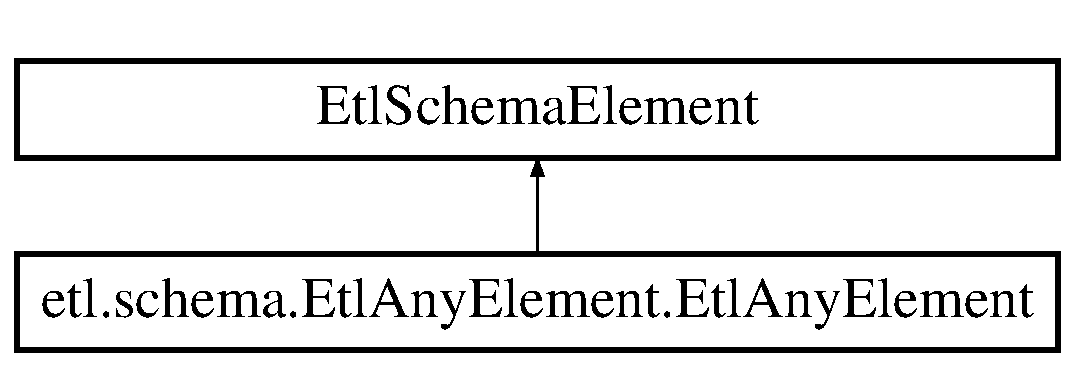
\includegraphics[height=2.000000cm]{classetl_1_1schema_1_1EtlAnyElement_1_1EtlAnyElement}
\end{center}
\end{figure}
\subsection*{Public Member Functions}
\begin{DoxyCompactItemize}
\item 
\hypertarget{classetl_1_1schema_1_1EtlAnyElement_1_1EtlAnyElement_af041ac2088b464cd3bf09b3380f9a10f}{def {\bfseries \-\_\-\-\_\-init\-\_\-\-\_\-}}\label{classetl_1_1schema_1_1EtlAnyElement_1_1EtlAnyElement_af041ac2088b464cd3bf09b3380f9a10f}

\end{DoxyCompactItemize}


\subsection{Detailed Description}
\begin{DoxyVerb}Don't want to specify the type of the field value?  Use this.\end{DoxyVerb}
 

The documentation for this class was generated from the following file\-:\begin{DoxyCompactItemize}
\item 
src/etl/schema/Etl\-Any\-Element.\-py\end{DoxyCompactItemize}

\hypertarget{classetl_1_1schema_1_1EtlBinaryElement_1_1EtlBinaryElement}{\section{etl.\-schema.\-Etl\-Binary\-Element.\-Etl\-Binary\-Element Class Reference}
\label{classetl_1_1schema_1_1EtlBinaryElement_1_1EtlBinaryElement}\index{etl.\-schema.\-Etl\-Binary\-Element.\-Etl\-Binary\-Element@{etl.\-schema.\-Etl\-Binary\-Element.\-Etl\-Binary\-Element}}
}
Inheritance diagram for etl.\-schema.\-Etl\-Binary\-Element.\-Etl\-Binary\-Element\-:\begin{figure}[H]
\begin{center}
\leavevmode
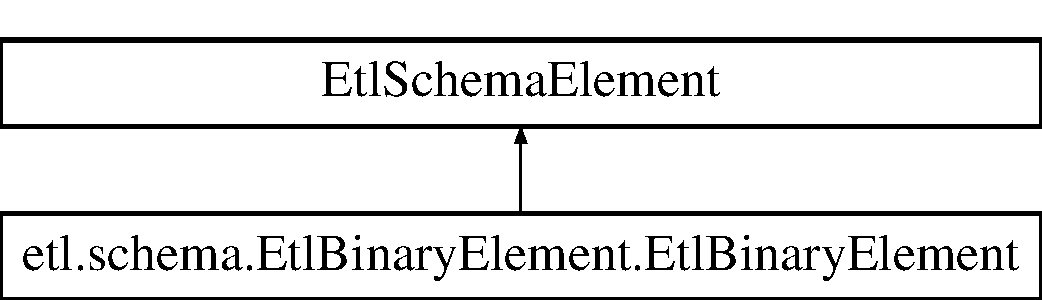
\includegraphics[height=2.000000cm]{classetl_1_1schema_1_1EtlBinaryElement_1_1EtlBinaryElement}
\end{center}
\end{figure}


\subsection{Detailed Description}
\begin{DoxyVerb}Any binary data (stored in memory)\end{DoxyVerb}
 

The documentation for this class was generated from the following file\-:\begin{DoxyCompactItemize}
\item 
src/etl/schema/Etl\-Binary\-Element.\-py\end{DoxyCompactItemize}

\hypertarget{classetl_1_1schema_1_1EtlBoolElement_1_1EtlBoolElement}{\section{etl.\-schema.\-Etl\-Bool\-Element.\-Etl\-Bool\-Element Class Reference}
\label{classetl_1_1schema_1_1EtlBoolElement_1_1EtlBoolElement}\index{etl.\-schema.\-Etl\-Bool\-Element.\-Etl\-Bool\-Element@{etl.\-schema.\-Etl\-Bool\-Element.\-Etl\-Bool\-Element}}
}
Inheritance diagram for etl.\-schema.\-Etl\-Bool\-Element.\-Etl\-Bool\-Element\-:\begin{figure}[H]
\begin{center}
\leavevmode
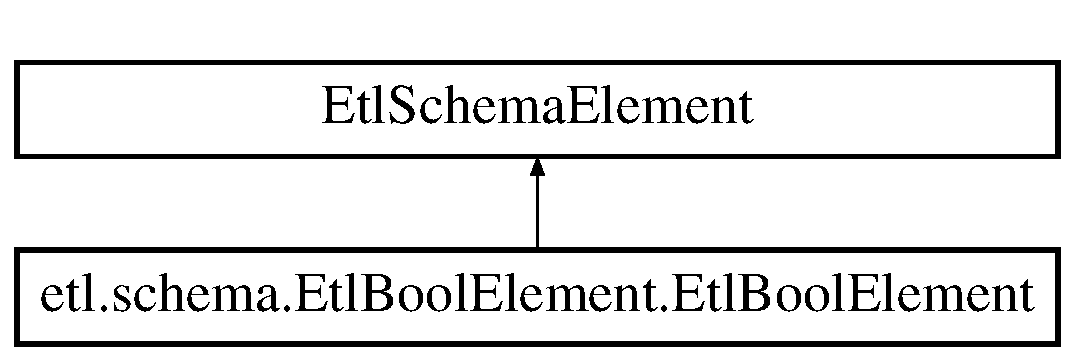
\includegraphics[height=2.000000cm]{classetl_1_1schema_1_1EtlBoolElement_1_1EtlBoolElement}
\end{center}
\end{figure}


\subsection{Detailed Description}
\begin{DoxyVerb}Yes/No values\end{DoxyVerb}
 

The documentation for this class was generated from the following file\-:\begin{DoxyCompactItemize}
\item 
src/etl/schema/Etl\-Bool\-Element.\-py\end{DoxyCompactItemize}

\hypertarget{classetl_1_1schema_1_1EtlIntElement_1_1EtlIntElement}{\section{etl.\-schema.\-Etl\-Int\-Element.\-Etl\-Int\-Element Class Reference}
\label{classetl_1_1schema_1_1EtlIntElement_1_1EtlIntElement}\index{etl.\-schema.\-Etl\-Int\-Element.\-Etl\-Int\-Element@{etl.\-schema.\-Etl\-Int\-Element.\-Etl\-Int\-Element}}
}
Inheritance diagram for etl.\-schema.\-Etl\-Int\-Element.\-Etl\-Int\-Element\-:\begin{figure}[H]
\begin{center}
\leavevmode
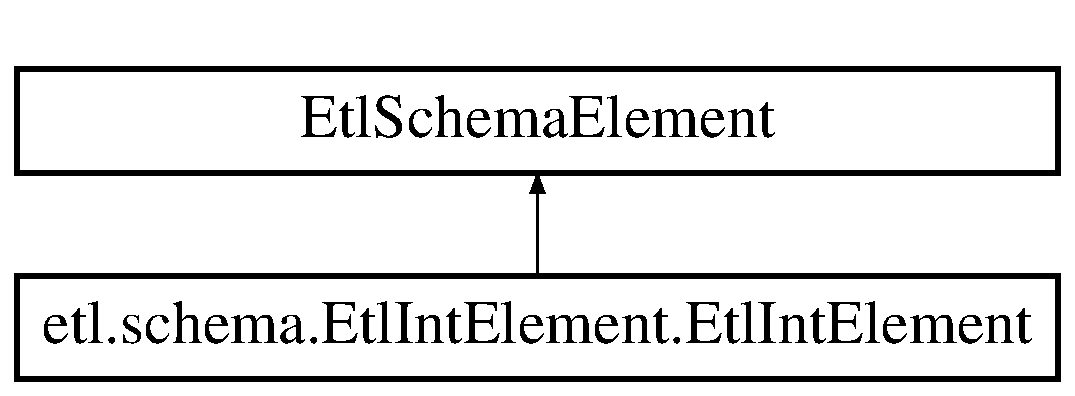
\includegraphics[height=2.000000cm]{classetl_1_1schema_1_1EtlIntElement_1_1EtlIntElement}
\end{center}
\end{figure}


\subsection{Detailed Description}
\begin{DoxyVerb}Integer values\end{DoxyVerb}
 

The documentation for this class was generated from the following file\-:\begin{DoxyCompactItemize}
\item 
src/etl/schema/Etl\-Int\-Element.\-py\end{DoxyCompactItemize}

\hypertarget{classetl_1_1schema_1_1EtlListElement_1_1EtlListElement}{\section{etl.\-schema.\-Etl\-List\-Element.\-Etl\-List\-Element Class Reference}
\label{classetl_1_1schema_1_1EtlListElement_1_1EtlListElement}\index{etl.\-schema.\-Etl\-List\-Element.\-Etl\-List\-Element@{etl.\-schema.\-Etl\-List\-Element.\-Etl\-List\-Element}}
}
Inheritance diagram for etl.\-schema.\-Etl\-List\-Element.\-Etl\-List\-Element\-:\begin{figure}[H]
\begin{center}
\leavevmode
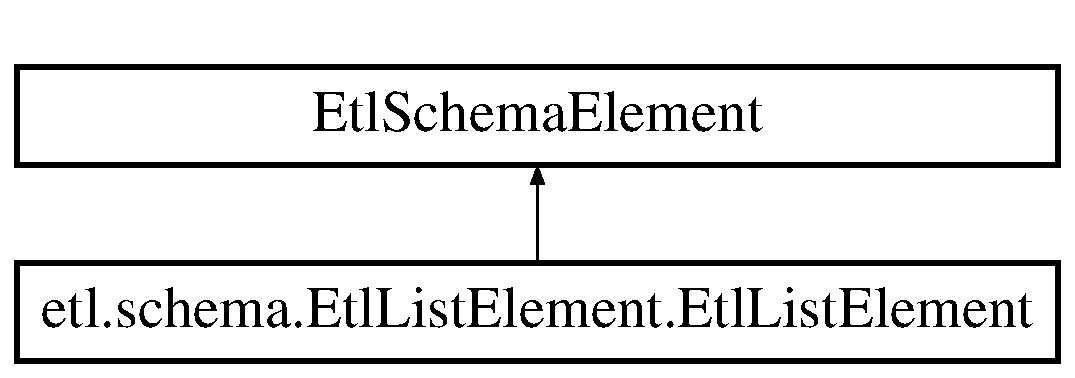
\includegraphics[height=2.000000cm]{classetl_1_1schema_1_1EtlListElement_1_1EtlListElement}
\end{center}
\end{figure}
\subsection*{Public Member Functions}
\begin{DoxyCompactItemize}
\item 
def \hyperlink{classetl_1_1schema_1_1EtlListElement_1_1EtlListElement_a3774caef17d71b25cffaef6da71a26ee}{\-\_\-\-\_\-init\-\_\-\-\_\-}
\item 
\hypertarget{classetl_1_1schema_1_1EtlListElement_1_1EtlListElement_a90c83ba5ed2b8367dcd5f81b9f047a6f}{def {\bfseries item\-\_\-element}}\label{classetl_1_1schema_1_1EtlListElement_1_1EtlListElement_a90c83ba5ed2b8367dcd5f81b9f047a6f}

\item 
\hypertarget{classetl_1_1schema_1_1EtlListElement_1_1EtlListElement_a528d1bbe3f09aa7c509c7f10d4c598a7}{def {\bfseries \-\_\-\-\_\-eq\-\_\-\-\_\-}}\label{classetl_1_1schema_1_1EtlListElement_1_1EtlListElement_a528d1bbe3f09aa7c509c7f10d4c598a7}

\end{DoxyCompactItemize}
\subsection*{Public Attributes}
\begin{DoxyCompactItemize}
\item 
\hypertarget{classetl_1_1schema_1_1EtlListElement_1_1EtlListElement_a0b3e124ce4ecb1bb3532af211ba7b9fe}{{\bfseries item\-\_\-element}}\label{classetl_1_1schema_1_1EtlListElement_1_1EtlListElement_a0b3e124ce4ecb1bb3532af211ba7b9fe}

\end{DoxyCompactItemize}


\subsection{Detailed Description}
\begin{DoxyVerb}An element that stores a list of items\end{DoxyVerb}
 

\subsection{Constructor \& Destructor Documentation}
\hypertarget{classetl_1_1schema_1_1EtlListElement_1_1EtlListElement_a3774caef17d71b25cffaef6da71a26ee}{\index{etl\-::schema\-::\-Etl\-List\-Element\-::\-Etl\-List\-Element@{etl\-::schema\-::\-Etl\-List\-Element\-::\-Etl\-List\-Element}!\-\_\-\-\_\-init\-\_\-\-\_\-@{\-\_\-\-\_\-init\-\_\-\-\_\-}}
\index{\-\_\-\-\_\-init\-\_\-\-\_\-@{\-\_\-\-\_\-init\-\_\-\-\_\-}!etl::schema::EtlListElement::EtlListElement@{etl\-::schema\-::\-Etl\-List\-Element\-::\-Etl\-List\-Element}}
\subsubsection[{\-\_\-\-\_\-init\-\_\-\-\_\-}]{\setlength{\rightskip}{0pt plus 5cm}def etl.\-schema.\-Etl\-List\-Element.\-Etl\-List\-Element.\-\_\-\-\_\-init\-\_\-\-\_\- (
\begin{DoxyParamCaption}
\item[{}]{self, }
\item[{}]{item\-\_\-element}
\end{DoxyParamCaption}
)}}\label{classetl_1_1schema_1_1EtlListElement_1_1EtlListElement_a3774caef17d71b25cffaef6da71a26ee}
\begin{DoxyVerb}Init 

@param item_element:
    An EtlSchemaElement for the items of the list
\end{DoxyVerb}
 

The documentation for this class was generated from the following file\-:\begin{DoxyCompactItemize}
\item 
src/etl/schema/Etl\-List\-Element.\-py\end{DoxyCompactItemize}

\hypertarget{classetl_1_1schema_1_1EtlRecordElement_1_1EtlRecordElement}{\section{etl.\-schema.\-Etl\-Record\-Element.\-Etl\-Record\-Element Class Reference}
\label{classetl_1_1schema_1_1EtlRecordElement_1_1EtlRecordElement}\index{etl.\-schema.\-Etl\-Record\-Element.\-Etl\-Record\-Element@{etl.\-schema.\-Etl\-Record\-Element.\-Etl\-Record\-Element}}
}
Inheritance diagram for etl.\-schema.\-Etl\-Record\-Element.\-Etl\-Record\-Element\-:\begin{figure}[H]
\begin{center}
\leavevmode
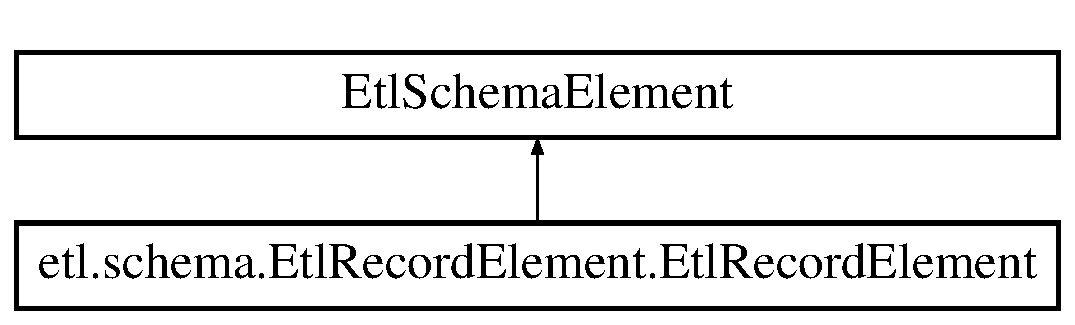
\includegraphics[height=2.000000cm]{classetl_1_1schema_1_1EtlRecordElement_1_1EtlRecordElement}
\end{center}
\end{figure}
\subsection*{Public Member Functions}
\begin{DoxyCompactItemize}
\item 
def \hyperlink{classetl_1_1schema_1_1EtlRecordElement_1_1EtlRecordElement_a976867350ebe6053980d47778c4cc8bb}{\-\_\-\-\_\-init\-\_\-\-\_\-}
\item 
\hypertarget{classetl_1_1schema_1_1EtlRecordElement_1_1EtlRecordElement_a849503de3f5681b4bc83faabeb4a1cb8}{def {\bfseries record\-\_\-schema}}\label{classetl_1_1schema_1_1EtlRecordElement_1_1EtlRecordElement_a849503de3f5681b4bc83faabeb4a1cb8}

\item 
\hypertarget{classetl_1_1schema_1_1EtlRecordElement_1_1EtlRecordElement_afed59b153c5627c20e7a12c36feb8a41}{def {\bfseries \-\_\-\-\_\-eq\-\_\-\-\_\-}}\label{classetl_1_1schema_1_1EtlRecordElement_1_1EtlRecordElement_afed59b153c5627c20e7a12c36feb8a41}

\end{DoxyCompactItemize}


\subsection{Detailed Description}
\begin{DoxyVerb}An element that stores a record\end{DoxyVerb}
 

\subsection{Constructor \& Destructor Documentation}
\hypertarget{classetl_1_1schema_1_1EtlRecordElement_1_1EtlRecordElement_a976867350ebe6053980d47778c4cc8bb}{\index{etl\-::schema\-::\-Etl\-Record\-Element\-::\-Etl\-Record\-Element@{etl\-::schema\-::\-Etl\-Record\-Element\-::\-Etl\-Record\-Element}!\-\_\-\-\_\-init\-\_\-\-\_\-@{\-\_\-\-\_\-init\-\_\-\-\_\-}}
\index{\-\_\-\-\_\-init\-\_\-\-\_\-@{\-\_\-\-\_\-init\-\_\-\-\_\-}!etl::schema::EtlRecordElement::EtlRecordElement@{etl\-::schema\-::\-Etl\-Record\-Element\-::\-Etl\-Record\-Element}}
\subsubsection[{\-\_\-\-\_\-init\-\_\-\-\_\-}]{\setlength{\rightskip}{0pt plus 5cm}def etl.\-schema.\-Etl\-Record\-Element.\-Etl\-Record\-Element.\-\_\-\-\_\-init\-\_\-\-\_\- (
\begin{DoxyParamCaption}
\item[{}]{self, }
\item[{}]{record\-\_\-schema}
\end{DoxyParamCaption}
)}}\label{classetl_1_1schema_1_1EtlRecordElement_1_1EtlRecordElement_a976867350ebe6053980d47778c4cc8bb}
\begin{DoxyVerb}Init 

@param record_schema:
    The schema of the record that this 
\end{DoxyVerb}
 

The documentation for this class was generated from the following file\-:\begin{DoxyCompactItemize}
\item 
src/etl/schema/Etl\-Record\-Element.\-py\end{DoxyCompactItemize}

\hypertarget{classetl_1_1schema_1_1EtlSchema_1_1EtlSchema}{\section{etl.\-schema.\-Etl\-Schema.\-Etl\-Schema Class Reference}
\label{classetl_1_1schema_1_1EtlSchema_1_1EtlSchema}\index{etl.\-schema.\-Etl\-Schema.\-Etl\-Schema@{etl.\-schema.\-Etl\-Schema.\-Etl\-Schema}}
}
Inheritance diagram for etl.\-schema.\-Etl\-Schema.\-Etl\-Schema\-:\begin{figure}[H]
\begin{center}
\leavevmode
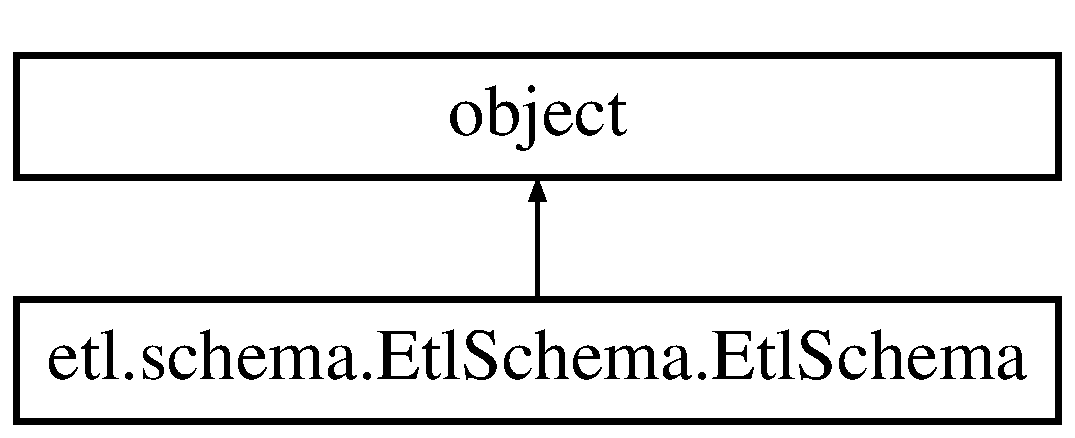
\includegraphics[height=2.000000cm]{classetl_1_1schema_1_1EtlSchema_1_1EtlSchema}
\end{center}
\end{figure}
\subsection*{Public Member Functions}
\begin{DoxyCompactItemize}
\item 
\hypertarget{classetl_1_1schema_1_1EtlSchema_1_1EtlSchema_ab7ab47ea64b7bd9030be721817da188c}{def {\bfseries \-\_\-\-\_\-init\-\_\-\-\_\-}}\label{classetl_1_1schema_1_1EtlSchema_1_1EtlSchema_ab7ab47ea64b7bd9030be721817da188c}

\item 
def \hyperlink{classetl_1_1schema_1_1EtlSchema_1_1EtlSchema_a689a98225755a0a2d65ac0015fabf2ee}{etl\-\_\-add\-\_\-field}
\item 
def \hyperlink{classetl_1_1schema_1_1EtlSchema_1_1EtlSchema_a18260552765b7f1eea45d12dab3eac70}{etl\-\_\-check\-\_\-record\-\_\-struct}
\item 
\hypertarget{classetl_1_1schema_1_1EtlSchema_1_1EtlSchema_a8c7059074731b52197d9574b21685fbe}{def {\bfseries etl\-\_\-list\-\_\-field\-\_\-names}}\label{classetl_1_1schema_1_1EtlSchema_1_1EtlSchema_a8c7059074731b52197d9574b21685fbe}

\item 
\hypertarget{classetl_1_1schema_1_1EtlSchema_1_1EtlSchema_a34e22026a19927cc8dfce59e62d4a343}{def {\bfseries etl\-\_\-list\-\_\-fields}}\label{classetl_1_1schema_1_1EtlSchema_1_1EtlSchema_a34e22026a19927cc8dfce59e62d4a343}

\item 
def \hyperlink{classetl_1_1schema_1_1EtlSchema_1_1EtlSchema_a5563f88b44d362bf39bab48a676188d1}{etl\-\_\-get\-\_\-field}
\item 
\hypertarget{classetl_1_1schema_1_1EtlSchema_1_1EtlSchema_ae9e1060ef06f9d36eca29b8658a31788}{def {\bfseries \-\_\-\-\_\-getitem\-\_\-\-\_\-}}\label{classetl_1_1schema_1_1EtlSchema_1_1EtlSchema_ae9e1060ef06f9d36eca29b8658a31788}

\item 
\hypertarget{classetl_1_1schema_1_1EtlSchema_1_1EtlSchema_af7c64e28f6d7c1c811dece2062797127}{def {\bfseries \-\_\-\-\_\-eq\-\_\-\-\_\-}}\label{classetl_1_1schema_1_1EtlSchema_1_1EtlSchema_af7c64e28f6d7c1c811dece2062797127}

\item 
\hypertarget{classetl_1_1schema_1_1EtlSchema_1_1EtlSchema_a98cd9c88bc62e5e3ee134accf1bbf863}{def {\bfseries \-\_\-\-\_\-str\-\_\-\-\_\-}}\label{classetl_1_1schema_1_1EtlSchema_1_1EtlSchema_a98cd9c88bc62e5e3ee134accf1bbf863}

\end{DoxyCompactItemize}
\subsection*{Static Public Attributes}
\begin{DoxyCompactItemize}
\item 
\hypertarget{classetl_1_1schema_1_1EtlSchema_1_1EtlSchema_a6990380c6563e54b77cd17987f7455f1}{string {\bfseries S\-T\-R\-I\-N\-G} = 'str'}\label{classetl_1_1schema_1_1EtlSchema_1_1EtlSchema_a6990380c6563e54b77cd17987f7455f1}

\item 
\hypertarget{classetl_1_1schema_1_1EtlSchema_1_1EtlSchema_a2e3f1e529b39da0902067c16166577a1}{string {\bfseries I\-N\-T} = 'int'}\label{classetl_1_1schema_1_1EtlSchema_1_1EtlSchema_a2e3f1e529b39da0902067c16166577a1}

\item 
\hypertarget{classetl_1_1schema_1_1EtlSchema_1_1EtlSchema_a4c5d98d168f7b7931f41b8782ad9cc88}{string {\bfseries F\-L\-O\-A\-T} = 'int'}\label{classetl_1_1schema_1_1EtlSchema_1_1EtlSchema_a4c5d98d168f7b7931f41b8782ad9cc88}

\item 
\hypertarget{classetl_1_1schema_1_1EtlSchema_1_1EtlSchema_a05959729ee7ceabff61ddb16dc1676b3}{string {\bfseries D\-A\-T\-E} = 'date'}\label{classetl_1_1schema_1_1EtlSchema_1_1EtlSchema_a05959729ee7ceabff61ddb16dc1676b3}

\item 
\hypertarget{classetl_1_1schema_1_1EtlSchema_1_1EtlSchema_a6ebd68d26a8234d1ee6f1a0af3c695e4}{string {\bfseries B\-O\-O\-L} = 'bool'}\label{classetl_1_1schema_1_1EtlSchema_1_1EtlSchema_a6ebd68d26a8234d1ee6f1a0af3c695e4}

\end{DoxyCompactItemize}


\subsection{Detailed Description}
\begin{DoxyVerb}Describes the structure of a record

The purpose of the schema is to assist the ETL logic with handling the
fields of records when the ETL library does not know the structure
of the records that will be used.  I've gone back and forth as to
whether to even require schemas, and whether to lock down input and
output ports to schemas.  Managing schemas, in my experience, can become
tedious and self-serving.

I've decided to keep schemas though to assist with:

    - Freezing records from changes
    - Serializeing records to disk
    - Debuging/Describing records to the user

I will not provide a mechanism to lock/check schemas on processor ports,
though, and I don't see a great advantage to requiring this.  This leaves
a processor to be flexible in recieving multiple record types if desired,
and leaves it up to the developer to ensure that the required fields for a
given processor are present.  I feel this supports the common Python
practice of Duck Typing.

Each record, however, does need to have an associated schema.
\end{DoxyVerb}
 

\subsection{Member Function Documentation}
\hypertarget{classetl_1_1schema_1_1EtlSchema_1_1EtlSchema_a689a98225755a0a2d65ac0015fabf2ee}{\index{etl\-::schema\-::\-Etl\-Schema\-::\-Etl\-Schema@{etl\-::schema\-::\-Etl\-Schema\-::\-Etl\-Schema}!etl\-\_\-add\-\_\-field@{etl\-\_\-add\-\_\-field}}
\index{etl\-\_\-add\-\_\-field@{etl\-\_\-add\-\_\-field}!etl::schema::EtlSchema::EtlSchema@{etl\-::schema\-::\-Etl\-Schema\-::\-Etl\-Schema}}
\subsubsection[{etl\-\_\-add\-\_\-field}]{\setlength{\rightskip}{0pt plus 5cm}def etl.\-schema.\-Etl\-Schema.\-Etl\-Schema.\-etl\-\_\-add\-\_\-field (
\begin{DoxyParamCaption}
\item[{}]{self, }
\item[{}]{name, }
\item[{}]{element\-\_\-class}
\end{DoxyParamCaption}
)}}\label{classetl_1_1schema_1_1EtlSchema_1_1EtlSchema_a689a98225755a0a2d65ac0015fabf2ee}
\begin{DoxyVerb}Add a field to the schema

@param name: Name of the field and field key in the records
@param desc: Long description of the field
@param header: Header to use when dumping records to a file
\end{DoxyVerb}
 \hypertarget{classetl_1_1schema_1_1EtlSchema_1_1EtlSchema_a18260552765b7f1eea45d12dab3eac70}{\index{etl\-::schema\-::\-Etl\-Schema\-::\-Etl\-Schema@{etl\-::schema\-::\-Etl\-Schema\-::\-Etl\-Schema}!etl\-\_\-check\-\_\-record\-\_\-struct@{etl\-\_\-check\-\_\-record\-\_\-struct}}
\index{etl\-\_\-check\-\_\-record\-\_\-struct@{etl\-\_\-check\-\_\-record\-\_\-struct}!etl::schema::EtlSchema::EtlSchema@{etl\-::schema\-::\-Etl\-Schema\-::\-Etl\-Schema}}
\subsubsection[{etl\-\_\-check\-\_\-record\-\_\-struct}]{\setlength{\rightskip}{0pt plus 5cm}def etl.\-schema.\-Etl\-Schema.\-Etl\-Schema.\-etl\-\_\-check\-\_\-record\-\_\-struct (
\begin{DoxyParamCaption}
\item[{}]{self, }
\item[{}]{record}
\end{DoxyParamCaption}
)}}\label{classetl_1_1schema_1_1EtlSchema_1_1EtlSchema_a18260552765b7f1eea45d12dab3eac70}
\begin{DoxyVerb}Check to see if the record matches this schema\end{DoxyVerb}
 \hypertarget{classetl_1_1schema_1_1EtlSchema_1_1EtlSchema_a5563f88b44d362bf39bab48a676188d1}{\index{etl\-::schema\-::\-Etl\-Schema\-::\-Etl\-Schema@{etl\-::schema\-::\-Etl\-Schema\-::\-Etl\-Schema}!etl\-\_\-get\-\_\-field@{etl\-\_\-get\-\_\-field}}
\index{etl\-\_\-get\-\_\-field@{etl\-\_\-get\-\_\-field}!etl::schema::EtlSchema::EtlSchema@{etl\-::schema\-::\-Etl\-Schema\-::\-Etl\-Schema}}
\subsubsection[{etl\-\_\-get\-\_\-field}]{\setlength{\rightskip}{0pt plus 5cm}def etl.\-schema.\-Etl\-Schema.\-Etl\-Schema.\-etl\-\_\-get\-\_\-field (
\begin{DoxyParamCaption}
\item[{}]{self, }
\item[{}]{name}
\end{DoxyParamCaption}
)}}\label{classetl_1_1schema_1_1EtlSchema_1_1EtlSchema_a5563f88b44d362bf39bab48a676188d1}
\begin{DoxyVerb}Get an element (field) of the schema by name\end{DoxyVerb}
 

The documentation for this class was generated from the following file\-:\begin{DoxyCompactItemize}
\item 
src/etl/schema/Etl\-Schema.\-py\end{DoxyCompactItemize}

\hypertarget{classetl_1_1schema_1_1EtlSchemaElement_1_1EtlSchemaElement}{\section{etl.\-schema.\-Etl\-Schema\-Element.\-Etl\-Schema\-Element Class Reference}
\label{classetl_1_1schema_1_1EtlSchemaElement_1_1EtlSchemaElement}\index{etl.\-schema.\-Etl\-Schema\-Element.\-Etl\-Schema\-Element@{etl.\-schema.\-Etl\-Schema\-Element.\-Etl\-Schema\-Element}}
}
Inheritance diagram for etl.\-schema.\-Etl\-Schema\-Element.\-Etl\-Schema\-Element\-:\begin{figure}[H]
\begin{center}
\leavevmode
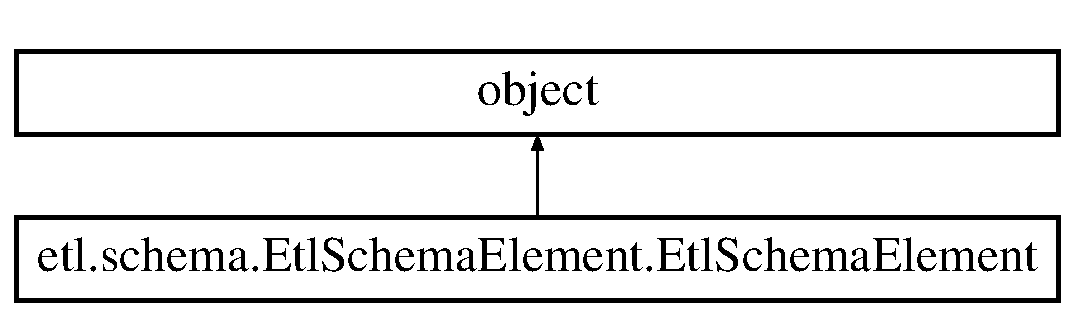
\includegraphics[height=2.000000cm]{classetl_1_1schema_1_1EtlSchemaElement_1_1EtlSchemaElement}
\end{center}
\end{figure}
\subsection*{Public Member Functions}
\begin{DoxyCompactItemize}
\item 
def \hyperlink{classetl_1_1schema_1_1EtlSchemaElement_1_1EtlSchemaElement_acbcff59a143bee00955e171565dcf872}{is\-\_\-schema\-\_\-element}
\item 
\hypertarget{classetl_1_1schema_1_1EtlSchemaElement_1_1EtlSchemaElement_a7ef81618ee68fb1cbf350ca9c9937215}{def {\bfseries element\-\_\-type\-\_\-code}}\label{classetl_1_1schema_1_1EtlSchemaElement_1_1EtlSchemaElement_a7ef81618ee68fb1cbf350ca9c9937215}

\item 
\hypertarget{classetl_1_1schema_1_1EtlSchemaElement_1_1EtlSchemaElement_a153d4c047df7b5b065f771a2116974fd}{def {\bfseries \-\_\-\-\_\-init\-\_\-\-\_\-}}\label{classetl_1_1schema_1_1EtlSchemaElement_1_1EtlSchemaElement_a153d4c047df7b5b065f771a2116974fd}

\item 
def \hyperlink{classetl_1_1schema_1_1EtlSchemaElement_1_1EtlSchemaElement_adcf1f1373de38cddd494fd604c33a01a}{set\-\_\-header}
\item 
\hypertarget{classetl_1_1schema_1_1EtlSchemaElement_1_1EtlSchemaElement_a352542775633524d4050c9054c7a5ece}{def {\bfseries \-\_\-\-\_\-eq\-\_\-\-\_\-}}\label{classetl_1_1schema_1_1EtlSchemaElement_1_1EtlSchemaElement_a352542775633524d4050c9054c7a5ece}

\item 
\hypertarget{classetl_1_1schema_1_1EtlSchemaElement_1_1EtlSchemaElement_ae59f607e19ac0f96fa53985eeb7ca243}{def {\bfseries \-\_\-\-\_\-str\-\_\-\-\_\-}}\label{classetl_1_1schema_1_1EtlSchemaElement_1_1EtlSchemaElement_ae59f607e19ac0f96fa53985eeb7ca243}

\end{DoxyCompactItemize}
\subsection*{Public Attributes}
\begin{DoxyCompactItemize}
\item 
\hypertarget{classetl_1_1schema_1_1EtlSchemaElement_1_1EtlSchemaElement_a471f578264e20df9962b2a3b4efbe2cc}{{\bfseries header}}\label{classetl_1_1schema_1_1EtlSchemaElement_1_1EtlSchemaElement_a471f578264e20df9962b2a3b4efbe2cc}

\end{DoxyCompactItemize}


\subsection{Detailed Description}
\begin{DoxyVerb}A field within a record

These classes assist the ETL process with knowing how to handle values.
They can also be used to specify constraints on the data that will be
used to identify records with errors.

Each attribute in a schema that represents a field in the record is an
instantiated EltSchemaElement object.  Values for fields are stored in the
EtlRecord object.
\end{DoxyVerb}
 

\subsection{Member Function Documentation}
\hypertarget{classetl_1_1schema_1_1EtlSchemaElement_1_1EtlSchemaElement_acbcff59a143bee00955e171565dcf872}{\index{etl\-::schema\-::\-Etl\-Schema\-Element\-::\-Etl\-Schema\-Element@{etl\-::schema\-::\-Etl\-Schema\-Element\-::\-Etl\-Schema\-Element}!is\-\_\-schema\-\_\-element@{is\-\_\-schema\-\_\-element}}
\index{is\-\_\-schema\-\_\-element@{is\-\_\-schema\-\_\-element}!etl::schema::EtlSchemaElement::EtlSchemaElement@{etl\-::schema\-::\-Etl\-Schema\-Element\-::\-Etl\-Schema\-Element}}
\subsubsection[{is\-\_\-schema\-\_\-element}]{\setlength{\rightskip}{0pt plus 5cm}def etl.\-schema.\-Etl\-Schema\-Element.\-Etl\-Schema\-Element.\-is\-\_\-schema\-\_\-element (
\begin{DoxyParamCaption}
\item[{}]{self}
\end{DoxyParamCaption}
)}}\label{classetl_1_1schema_1_1EtlSchemaElement_1_1EtlSchemaElement_acbcff59a143bee00955e171565dcf872}
\begin{DoxyVerb}Marker to tell other ETL code that this is a schema element\end{DoxyVerb}
 \hypertarget{classetl_1_1schema_1_1EtlSchemaElement_1_1EtlSchemaElement_adcf1f1373de38cddd494fd604c33a01a}{\index{etl\-::schema\-::\-Etl\-Schema\-Element\-::\-Etl\-Schema\-Element@{etl\-::schema\-::\-Etl\-Schema\-Element\-::\-Etl\-Schema\-Element}!set\-\_\-header@{set\-\_\-header}}
\index{set\-\_\-header@{set\-\_\-header}!etl::schema::EtlSchemaElement::EtlSchemaElement@{etl\-::schema\-::\-Etl\-Schema\-Element\-::\-Etl\-Schema\-Element}}
\subsubsection[{set\-\_\-header}]{\setlength{\rightskip}{0pt plus 5cm}def etl.\-schema.\-Etl\-Schema\-Element.\-Etl\-Schema\-Element.\-set\-\_\-header (
\begin{DoxyParamCaption}
\item[{}]{self, }
\item[{}]{value}
\end{DoxyParamCaption}
)}}\label{classetl_1_1schema_1_1EtlSchemaElement_1_1EtlSchemaElement_adcf1f1373de38cddd494fd604c33a01a}
\begin{DoxyVerb}Set the column header used when describing this field\end{DoxyVerb}
 

The documentation for this class was generated from the following file\-:\begin{DoxyCompactItemize}
\item 
src/etl/schema/Etl\-Schema\-Element.\-py\end{DoxyCompactItemize}

\hypertarget{classetl_1_1schema_1_1EtlStringElement_1_1EtlStringElement}{\section{etl.\-schema.\-Etl\-String\-Element.\-Etl\-String\-Element Class Reference}
\label{classetl_1_1schema_1_1EtlStringElement_1_1EtlStringElement}\index{etl.\-schema.\-Etl\-String\-Element.\-Etl\-String\-Element@{etl.\-schema.\-Etl\-String\-Element.\-Etl\-String\-Element}}
}
Inheritance diagram for etl.\-schema.\-Etl\-String\-Element.\-Etl\-String\-Element\-:\begin{figure}[H]
\begin{center}
\leavevmode
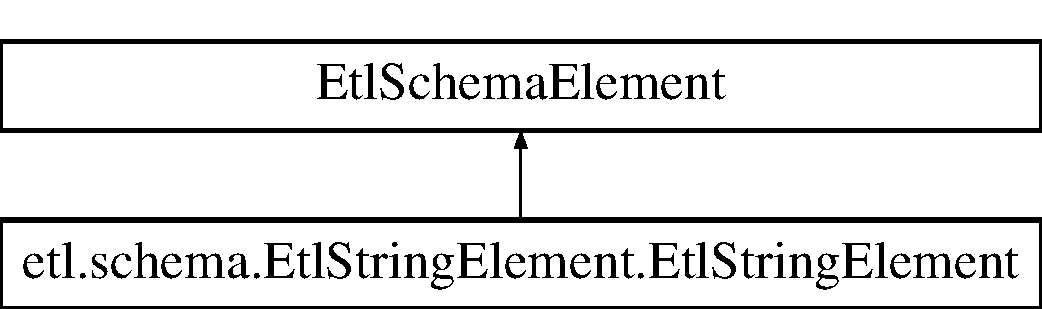
\includegraphics[height=2.000000cm]{classetl_1_1schema_1_1EtlStringElement_1_1EtlStringElement}
\end{center}
\end{figure}
\subsection*{Public Member Functions}
\begin{DoxyCompactItemize}
\item 
\hypertarget{classetl_1_1schema_1_1EtlStringElement_1_1EtlStringElement_ac0083f4dffbce05bcd19a6c3abb6c565}{def {\bfseries \-\_\-\-\_\-init\-\_\-\-\_\-}}\label{classetl_1_1schema_1_1EtlStringElement_1_1EtlStringElement_ac0083f4dffbce05bcd19a6c3abb6c565}

\item 
\hypertarget{classetl_1_1schema_1_1EtlStringElement_1_1EtlStringElement_ab3afd9e24dd1e7c3fc11411b3e72b7ad}{def {\bfseries \-\_\-\-\_\-eq\-\_\-\-\_\-}}\label{classetl_1_1schema_1_1EtlStringElement_1_1EtlStringElement_ab3afd9e24dd1e7c3fc11411b3e72b7ad}

\end{DoxyCompactItemize}
\subsection*{Public Attributes}
\begin{DoxyCompactItemize}
\item 
\hypertarget{classetl_1_1schema_1_1EtlStringElement_1_1EtlStringElement_aab58b4a15650b65087d0d237b0d9dd7b}{{\bfseries max\-\_\-length}}\label{classetl_1_1schema_1_1EtlStringElement_1_1EtlStringElement_aab58b4a15650b65087d0d237b0d9dd7b}

\end{DoxyCompactItemize}


\subsection{Detailed Description}
\begin{DoxyVerb}String values\end{DoxyVerb}
 

The documentation for this class was generated from the following file\-:\begin{DoxyCompactItemize}
\item 
src/etl/schema/Etl\-String\-Element.\-py\end{DoxyCompactItemize}

\hypertarget{classetl_1_1tk__monitor_1_1PrcStatusGridComponents_1_1DataPortInGrid}{\section{etl.\-tk\-\_\-monitor.\-Prc\-Status\-Grid\-Components.\-Data\-Port\-In\-Grid Class Reference}
\label{classetl_1_1tk__monitor_1_1PrcStatusGridComponents_1_1DataPortInGrid}\index{etl.\-tk\-\_\-monitor.\-Prc\-Status\-Grid\-Components.\-Data\-Port\-In\-Grid@{etl.\-tk\-\_\-monitor.\-Prc\-Status\-Grid\-Components.\-Data\-Port\-In\-Grid}}
}
Inheritance diagram for etl.\-tk\-\_\-monitor.\-Prc\-Status\-Grid\-Components.\-Data\-Port\-In\-Grid\-:\begin{figure}[H]
\begin{center}
\leavevmode
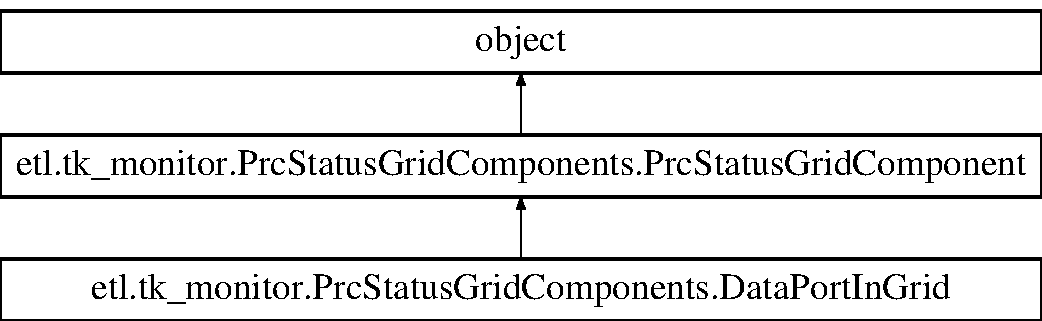
\includegraphics[height=3.000000cm]{classetl_1_1tk__monitor_1_1PrcStatusGridComponents_1_1DataPortInGrid}
\end{center}
\end{figure}
\subsection*{Public Member Functions}
\begin{DoxyCompactItemize}
\item 
\hypertarget{classetl_1_1tk__monitor_1_1PrcStatusGridComponents_1_1DataPortInGrid_a3cb0353b45a094855969e8dc524005b4}{def {\bfseries \-\_\-\-\_\-init\-\_\-\-\_\-}}\label{classetl_1_1tk__monitor_1_1PrcStatusGridComponents_1_1DataPortInGrid_a3cb0353b45a094855969e8dc524005b4}

\end{DoxyCompactItemize}
\subsection*{Public Attributes}
\begin{DoxyCompactItemize}
\item 
\hypertarget{classetl_1_1tk__monitor_1_1PrcStatusGridComponents_1_1DataPortInGrid_a0dda1bb137876ea2ed9518e79102e8b9}{{\bfseries prc}}\label{classetl_1_1tk__monitor_1_1PrcStatusGridComponents_1_1DataPortInGrid_a0dda1bb137876ea2ed9518e79102e8b9}

\item 
\hypertarget{classetl_1_1tk__monitor_1_1PrcStatusGridComponents_1_1DataPortInGrid_ad646dfae20613f06e2999d28f0b8b080}{{\bfseries port}}\label{classetl_1_1tk__monitor_1_1PrcStatusGridComponents_1_1DataPortInGrid_ad646dfae20613f06e2999d28f0b8b080}

\item 
\hypertarget{classetl_1_1tk__monitor_1_1PrcStatusGridComponents_1_1DataPortInGrid_ae76425d3f5f6075c97debef72fe1aadf}{{\bfseries direction}}\label{classetl_1_1tk__monitor_1_1PrcStatusGridComponents_1_1DataPortInGrid_ae76425d3f5f6075c97debef72fe1aadf}

\item 
\hypertarget{classetl_1_1tk__monitor_1_1PrcStatusGridComponents_1_1DataPortInGrid_a6236b5d66cefe0349b9af7f619e25ae4}{{\bfseries direction\-\_\-abbrv}}\label{classetl_1_1tk__monitor_1_1PrcStatusGridComponents_1_1DataPortInGrid_a6236b5d66cefe0349b9af7f619e25ae4}

\item 
\hypertarget{classetl_1_1tk__monitor_1_1PrcStatusGridComponents_1_1DataPortInGrid_ae9589c5ad10b9b9fb34fe63ffe0eb7b6}{{\bfseries name\-\_\-var}}\label{classetl_1_1tk__monitor_1_1PrcStatusGridComponents_1_1DataPortInGrid_ae9589c5ad10b9b9fb34fe63ffe0eb7b6}

\item 
\hypertarget{classetl_1_1tk__monitor_1_1PrcStatusGridComponents_1_1DataPortInGrid_a4f3eb1a8bbaf04475a2f6a87a11fa16a}{{\bfseries name\-\_\-label}}\label{classetl_1_1tk__monitor_1_1PrcStatusGridComponents_1_1DataPortInGrid_a4f3eb1a8bbaf04475a2f6a87a11fa16a}

\item 
\hypertarget{classetl_1_1tk__monitor_1_1PrcStatusGridComponents_1_1DataPortInGrid_a8a3b3d6687434153a5fb7590a45754e2}{{\bfseries schema\-\_\-var}}\label{classetl_1_1tk__monitor_1_1PrcStatusGridComponents_1_1DataPortInGrid_a8a3b3d6687434153a5fb7590a45754e2}

\item 
\hypertarget{classetl_1_1tk__monitor_1_1PrcStatusGridComponents_1_1DataPortInGrid_acd40fadd12396e0cdf3df133002cd560}{{\bfseries schema\-\_\-label}}\label{classetl_1_1tk__monitor_1_1PrcStatusGridComponents_1_1DataPortInGrid_acd40fadd12396e0cdf3df133002cd560}

\item 
\hypertarget{classetl_1_1tk__monitor_1_1PrcStatusGridComponents_1_1DataPortInGrid_abbdaea15df60b10b28055095cc527ccb}{{\bfseries buffered\-\_\-var}}\label{classetl_1_1tk__monitor_1_1PrcStatusGridComponents_1_1DataPortInGrid_abbdaea15df60b10b28055095cc527ccb}

\item 
\hypertarget{classetl_1_1tk__monitor_1_1PrcStatusGridComponents_1_1DataPortInGrid_af7733c0942059803d1ba14e908155efd}{{\bfseries buffered\-\_\-label}}\label{classetl_1_1tk__monitor_1_1PrcStatusGridComponents_1_1DataPortInGrid_af7733c0942059803d1ba14e908155efd}

\item 
\hypertarget{classetl_1_1tk__monitor_1_1PrcStatusGridComponents_1_1DataPortInGrid_a8a8da5682a801bd0e660e4c70903b239}{{\bfseries count\-\_\-var}}\label{classetl_1_1tk__monitor_1_1PrcStatusGridComponents_1_1DataPortInGrid_a8a8da5682a801bd0e660e4c70903b239}

\item 
\hypertarget{classetl_1_1tk__monitor_1_1PrcStatusGridComponents_1_1DataPortInGrid_a3d638ac7841be52253dc39c0236d26c6}{{\bfseries count\-\_\-label}}\label{classetl_1_1tk__monitor_1_1PrcStatusGridComponents_1_1DataPortInGrid_a3d638ac7841be52253dc39c0236d26c6}

\end{DoxyCompactItemize}


\subsection{Detailed Description}
\begin{DoxyVerb}Holds the TK elements used to describe the status of a data port\end{DoxyVerb}
 

The documentation for this class was generated from the following file\-:\begin{DoxyCompactItemize}
\item 
src/etl/tk\-\_\-monitor/Prc\-Status\-Grid\-Components.\-py\end{DoxyCompactItemize}

\hypertarget{classetl_1_1tk__monitor_1_1PrcStatusGridComponents_1_1PrcStatusGridComponent}{\section{etl.\-tk\-\_\-monitor.\-Prc\-Status\-Grid\-Components.\-Prc\-Status\-Grid\-Component Class Reference}
\label{classetl_1_1tk__monitor_1_1PrcStatusGridComponents_1_1PrcStatusGridComponent}\index{etl.\-tk\-\_\-monitor.\-Prc\-Status\-Grid\-Components.\-Prc\-Status\-Grid\-Component@{etl.\-tk\-\_\-monitor.\-Prc\-Status\-Grid\-Components.\-Prc\-Status\-Grid\-Component}}
}
Inheritance diagram for etl.\-tk\-\_\-monitor.\-Prc\-Status\-Grid\-Components.\-Prc\-Status\-Grid\-Component\-:\begin{figure}[H]
\begin{center}
\leavevmode
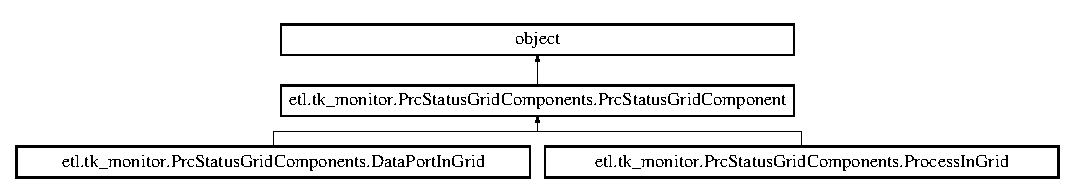
\includegraphics[height=2.153846cm]{classetl_1_1tk__monitor_1_1PrcStatusGridComponents_1_1PrcStatusGridComponent}
\end{center}
\end{figure}
\subsection*{Public Member Functions}
\begin{DoxyCompactItemize}
\item 
\hypertarget{classetl_1_1tk__monitor_1_1PrcStatusGridComponents_1_1PrcStatusGridComponent_afed3970b9f7beb4d6bf64438adc09b22}{def {\bfseries \-\_\-\-\_\-init\-\_\-\-\_\-}}\label{classetl_1_1tk__monitor_1_1PrcStatusGridComponents_1_1PrcStatusGridComponent_afed3970b9f7beb4d6bf64438adc09b22}

\end{DoxyCompactItemize}


The documentation for this class was generated from the following file\-:\begin{DoxyCompactItemize}
\item 
src/etl/tk\-\_\-monitor/Prc\-Status\-Grid\-Components.\-py\end{DoxyCompactItemize}

\hypertarget{classetl_1_1tk__monitor_1_1PrcStatusGridComponents_1_1ProcessInGrid}{\section{etl.\-tk\-\_\-monitor.\-Prc\-Status\-Grid\-Components.\-Process\-In\-Grid Class Reference}
\label{classetl_1_1tk__monitor_1_1PrcStatusGridComponents_1_1ProcessInGrid}\index{etl.\-tk\-\_\-monitor.\-Prc\-Status\-Grid\-Components.\-Process\-In\-Grid@{etl.\-tk\-\_\-monitor.\-Prc\-Status\-Grid\-Components.\-Process\-In\-Grid}}
}
Inheritance diagram for etl.\-tk\-\_\-monitor.\-Prc\-Status\-Grid\-Components.\-Process\-In\-Grid\-:\begin{figure}[H]
\begin{center}
\leavevmode
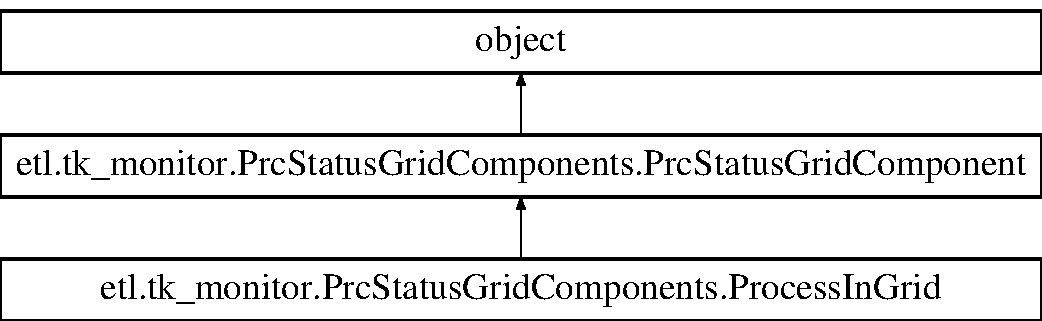
\includegraphics[height=3.000000cm]{classetl_1_1tk__monitor_1_1PrcStatusGridComponents_1_1ProcessInGrid}
\end{center}
\end{figure}
\subsection*{Public Member Functions}
\begin{DoxyCompactItemize}
\item 
\hypertarget{classetl_1_1tk__monitor_1_1PrcStatusGridComponents_1_1ProcessInGrid_ae15b56054378b76c33844086ac326c1a}{def {\bfseries \-\_\-\-\_\-init\-\_\-\-\_\-}}\label{classetl_1_1tk__monitor_1_1PrcStatusGridComponents_1_1ProcessInGrid_ae15b56054378b76c33844086ac326c1a}

\end{DoxyCompactItemize}
\subsection*{Public Attributes}
\begin{DoxyCompactItemize}
\item 
\hypertarget{classetl_1_1tk__monitor_1_1PrcStatusGridComponents_1_1ProcessInGrid_ad5aa4916ef59dfa9ac2faff821096537}{{\bfseries prc}}\label{classetl_1_1tk__monitor_1_1PrcStatusGridComponents_1_1ProcessInGrid_ad5aa4916ef59dfa9ac2faff821096537}

\item 
\hypertarget{classetl_1_1tk__monitor_1_1PrcStatusGridComponents_1_1ProcessInGrid_ab827370db44b30b2bdebd5fa736be13f}{{\bfseries prc\-\_\-var}}\label{classetl_1_1tk__monitor_1_1PrcStatusGridComponents_1_1ProcessInGrid_ab827370db44b30b2bdebd5fa736be13f}

\item 
\hypertarget{classetl_1_1tk__monitor_1_1PrcStatusGridComponents_1_1ProcessInGrid_abd102cee8367ca33598fdf9123bdbba7}{{\bfseries prc\-\_\-label}}\label{classetl_1_1tk__monitor_1_1PrcStatusGridComponents_1_1ProcessInGrid_abd102cee8367ca33598fdf9123bdbba7}

\item 
\hypertarget{classetl_1_1tk__monitor_1_1PrcStatusGridComponents_1_1ProcessInGrid_af742abaabe45ecef786887021a99b1d2}{{\bfseries prc\-\_\-class\-\_\-var}}\label{classetl_1_1tk__monitor_1_1PrcStatusGridComponents_1_1ProcessInGrid_af742abaabe45ecef786887021a99b1d2}

\item 
\hypertarget{classetl_1_1tk__monitor_1_1PrcStatusGridComponents_1_1ProcessInGrid_accd1a1d584d7d8e8cef1f97e88c284ed}{{\bfseries prc\-\_\-class\-\_\-label}}\label{classetl_1_1tk__monitor_1_1PrcStatusGridComponents_1_1ProcessInGrid_accd1a1d584d7d8e8cef1f97e88c284ed}

\item 
\hypertarget{classetl_1_1tk__monitor_1_1PrcStatusGridComponents_1_1ProcessInGrid_ae53b51c920623abe39d11775aeeb8d50}{{\bfseries prc\-\_\-status\-\_\-var}}\label{classetl_1_1tk__monitor_1_1PrcStatusGridComponents_1_1ProcessInGrid_ae53b51c920623abe39d11775aeeb8d50}

\item 
\hypertarget{classetl_1_1tk__monitor_1_1PrcStatusGridComponents_1_1ProcessInGrid_a9ad287cfcc0750b3122bdb66e5138fd5}{{\bfseries prc\-\_\-status\-\_\-label}}\label{classetl_1_1tk__monitor_1_1PrcStatusGridComponents_1_1ProcessInGrid_a9ad287cfcc0750b3122bdb66e5138fd5}

\item 
\hypertarget{classetl_1_1tk__monitor_1_1PrcStatusGridComponents_1_1ProcessInGrid_a9b9bf20b632cc50881e5d1b02bda92da}{{\bfseries inputs}}\label{classetl_1_1tk__monitor_1_1PrcStatusGridComponents_1_1ProcessInGrid_a9b9bf20b632cc50881e5d1b02bda92da}

\item 
\hypertarget{classetl_1_1tk__monitor_1_1PrcStatusGridComponents_1_1ProcessInGrid_a967fefc47730d901087ed474596e397f}{{\bfseries outputs}}\label{classetl_1_1tk__monitor_1_1PrcStatusGridComponents_1_1ProcessInGrid_a967fefc47730d901087ed474596e397f}

\end{DoxyCompactItemize}


\subsection{Detailed Description}
\begin{DoxyVerb}Holds the TK elements used to describe the status of a processor\end{DoxyVerb}
 

The documentation for this class was generated from the following file\-:\begin{DoxyCompactItemize}
\item 
src/etl/tk\-\_\-monitor/Prc\-Status\-Grid\-Components.\-py\end{DoxyCompactItemize}

\hypertarget{classetl_1_1tk__monitor_1_1TkProcessorStatusGrid_1_1TkProcessorStatusGrid}{\section{etl.\-tk\-\_\-monitor.\-Tk\-Processor\-Status\-Grid.\-Tk\-Processor\-Status\-Grid Class Reference}
\label{classetl_1_1tk__monitor_1_1TkProcessorStatusGrid_1_1TkProcessorStatusGrid}\index{etl.\-tk\-\_\-monitor.\-Tk\-Processor\-Status\-Grid.\-Tk\-Processor\-Status\-Grid@{etl.\-tk\-\_\-monitor.\-Tk\-Processor\-Status\-Grid.\-Tk\-Processor\-Status\-Grid}}
}
Inheritance diagram for etl.\-tk\-\_\-monitor.\-Tk\-Processor\-Status\-Grid.\-Tk\-Processor\-Status\-Grid\-:\begin{figure}[H]
\begin{center}
\leavevmode
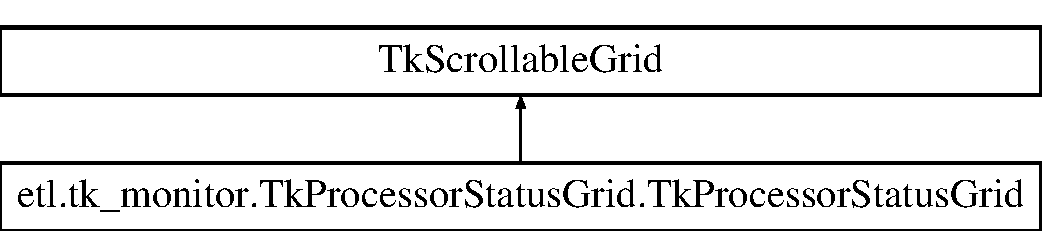
\includegraphics[height=2.000000cm]{classetl_1_1tk__monitor_1_1TkProcessorStatusGrid_1_1TkProcessorStatusGrid}
\end{center}
\end{figure}
\subsection*{Public Member Functions}
\begin{DoxyCompactItemize}
\item 
\hypertarget{classetl_1_1tk__monitor_1_1TkProcessorStatusGrid_1_1TkProcessorStatusGrid_ade5afc25ec51148040cfb25eb33684fe}{def {\bfseries \-\_\-\-\_\-init\-\_\-\-\_\-}}\label{classetl_1_1tk__monitor_1_1TkProcessorStatusGrid_1_1TkProcessorStatusGrid_ade5afc25ec51148040cfb25eb33684fe}

\item 
def \hyperlink{classetl_1_1tk__monitor_1_1TkProcessorStatusGrid_1_1TkProcessorStatusGrid_ac27896e2b7af840fc8caa646ad0f3763}{get\-\_\-labels\-\_\-for\-\_\-grid}
\item 
def \hyperlink{classetl_1_1tk__monitor_1_1TkProcessorStatusGrid_1_1TkProcessorStatusGrid_a836630b3c2d0588bcbf19c344c285d37}{get\-\_\-labels\-\_\-for\-\_\-prc\-\_\-on\-\_\-grid}
\end{DoxyCompactItemize}


\subsection{Detailed Description}
\begin{DoxyVerb}A scrollable grid showing the status of all processors\end{DoxyVerb}
 

\subsection{Member Function Documentation}
\hypertarget{classetl_1_1tk__monitor_1_1TkProcessorStatusGrid_1_1TkProcessorStatusGrid_ac27896e2b7af840fc8caa646ad0f3763}{\index{etl\-::tk\-\_\-monitor\-::\-Tk\-Processor\-Status\-Grid\-::\-Tk\-Processor\-Status\-Grid@{etl\-::tk\-\_\-monitor\-::\-Tk\-Processor\-Status\-Grid\-::\-Tk\-Processor\-Status\-Grid}!get\-\_\-labels\-\_\-for\-\_\-grid@{get\-\_\-labels\-\_\-for\-\_\-grid}}
\index{get\-\_\-labels\-\_\-for\-\_\-grid@{get\-\_\-labels\-\_\-for\-\_\-grid}!etl::tk_monitor::TkProcessorStatusGrid::TkProcessorStatusGrid@{etl\-::tk\-\_\-monitor\-::\-Tk\-Processor\-Status\-Grid\-::\-Tk\-Processor\-Status\-Grid}}
\subsubsection[{get\-\_\-labels\-\_\-for\-\_\-grid}]{\setlength{\rightskip}{0pt plus 5cm}def etl.\-tk\-\_\-monitor.\-Tk\-Processor\-Status\-Grid.\-Tk\-Processor\-Status\-Grid.\-get\-\_\-labels\-\_\-for\-\_\-grid (
\begin{DoxyParamCaption}
\item[{}]{self}
\end{DoxyParamCaption}
)}}\label{classetl_1_1tk__monitor_1_1TkProcessorStatusGrid_1_1TkProcessorStatusGrid_ac27896e2b7af840fc8caa646ad0f3763}
\begin{DoxyVerb}Return label widgets to place on grid in format

Keep in mind structure is 1 processor to many dataports
The current layout is:
    prc_fields    dataport_fields
          dataport_fields
    prc_fields    dataport_fields
          dataport_fields
          dataport_fields
          
@return list of fields with None where no label should be placed
\end{DoxyVerb}
 \hypertarget{classetl_1_1tk__monitor_1_1TkProcessorStatusGrid_1_1TkProcessorStatusGrid_a836630b3c2d0588bcbf19c344c285d37}{\index{etl\-::tk\-\_\-monitor\-::\-Tk\-Processor\-Status\-Grid\-::\-Tk\-Processor\-Status\-Grid@{etl\-::tk\-\_\-monitor\-::\-Tk\-Processor\-Status\-Grid\-::\-Tk\-Processor\-Status\-Grid}!get\-\_\-labels\-\_\-for\-\_\-prc\-\_\-on\-\_\-grid@{get\-\_\-labels\-\_\-for\-\_\-prc\-\_\-on\-\_\-grid}}
\index{get\-\_\-labels\-\_\-for\-\_\-prc\-\_\-on\-\_\-grid@{get\-\_\-labels\-\_\-for\-\_\-prc\-\_\-on\-\_\-grid}!etl::tk_monitor::TkProcessorStatusGrid::TkProcessorStatusGrid@{etl\-::tk\-\_\-monitor\-::\-Tk\-Processor\-Status\-Grid\-::\-Tk\-Processor\-Status\-Grid}}
\subsubsection[{get\-\_\-labels\-\_\-for\-\_\-prc\-\_\-on\-\_\-grid}]{\setlength{\rightskip}{0pt plus 5cm}def etl.\-tk\-\_\-monitor.\-Tk\-Processor\-Status\-Grid.\-Tk\-Processor\-Status\-Grid.\-get\-\_\-labels\-\_\-for\-\_\-prc\-\_\-on\-\_\-grid (
\begin{DoxyParamCaption}
\item[{}]{self, }
\item[{}]{prc\-\_\-comp}
\end{DoxyParamCaption}
)}}\label{classetl_1_1tk__monitor_1_1TkProcessorStatusGrid_1_1TkProcessorStatusGrid_a836630b3c2d0588bcbf19c344c285d37}
\begin{DoxyVerb}Return label widgets to place on grid for all dataport for a prc

This returns just the dataport field labels\end{DoxyVerb}
 

The documentation for this class was generated from the following file\-:\begin{DoxyCompactItemize}
\item 
src/etl/tk\-\_\-monitor/Tk\-Processor\-Status\-Grid.\-py\end{DoxyCompactItemize}

\hypertarget{classetl_1_1tk__monitor_1_1TkScrollableGrid_1_1TkScrollableGrid}{\section{etl.\-tk\-\_\-monitor.\-Tk\-Scrollable\-Grid.\-Tk\-Scrollable\-Grid Class Reference}
\label{classetl_1_1tk__monitor_1_1TkScrollableGrid_1_1TkScrollableGrid}\index{etl.\-tk\-\_\-monitor.\-Tk\-Scrollable\-Grid.\-Tk\-Scrollable\-Grid@{etl.\-tk\-\_\-monitor.\-Tk\-Scrollable\-Grid.\-Tk\-Scrollable\-Grid}}
}
Inheritance diagram for etl.\-tk\-\_\-monitor.\-Tk\-Scrollable\-Grid.\-Tk\-Scrollable\-Grid\-:\begin{figure}[H]
\begin{center}
\leavevmode
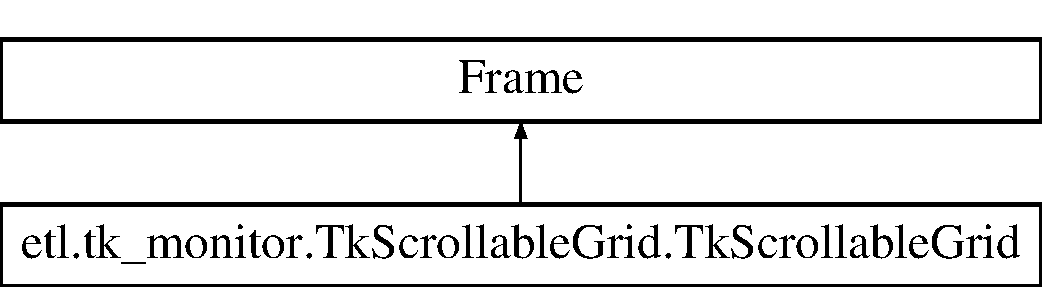
\includegraphics[height=2.000000cm]{classetl_1_1tk__monitor_1_1TkScrollableGrid_1_1TkScrollableGrid}
\end{center}
\end{figure}
\subsection*{Public Member Functions}
\begin{DoxyCompactItemize}
\item 
\hypertarget{classetl_1_1tk__monitor_1_1TkScrollableGrid_1_1TkScrollableGrid_ac88cc63c49d0bed587f27fd4d57a3dea}{def {\bfseries \-\_\-\-\_\-init\-\_\-\-\_\-}}\label{classetl_1_1tk__monitor_1_1TkScrollableGrid_1_1TkScrollableGrid_ac88cc63c49d0bed587f27fd4d57a3dea}

\item 
def \hyperlink{classetl_1_1tk__monitor_1_1TkScrollableGrid_1_1TkScrollableGrid_ac2c2852e023f92cd0d5ddfab66720171}{add\-\_\-column}
\item 
\hypertarget{classetl_1_1tk__monitor_1_1TkScrollableGrid_1_1TkScrollableGrid_a45efa9c10db2ec8ca90669eef8747162}{def {\bfseries get\-\_\-col\-\_\-name\-\_\-by\-\_\-pos}}\label{classetl_1_1tk__monitor_1_1TkScrollableGrid_1_1TkScrollableGrid_a45efa9c10db2ec8ca90669eef8747162}

\item 
\hypertarget{classetl_1_1tk__monitor_1_1TkScrollableGrid_1_1TkScrollableGrid_adcc4c0fee7d02a920da8cd70e59d69f5}{def {\bfseries add\-\_\-row}}\label{classetl_1_1tk__monitor_1_1TkScrollableGrid_1_1TkScrollableGrid_adcc4c0fee7d02a920da8cd70e59d69f5}

\item 
\hypertarget{classetl_1_1tk__monitor_1_1TkScrollableGrid_1_1TkScrollableGrid_ae802ce49a5413708c74ec1bfe3a24329}{def {\bfseries set\-\_\-value}}\label{classetl_1_1tk__monitor_1_1TkScrollableGrid_1_1TkScrollableGrid_ae802ce49a5413708c74ec1bfe3a24329}

\item 
\hypertarget{classetl_1_1tk__monitor_1_1TkScrollableGrid_1_1TkScrollableGrid_abf5fff1a9640616ef7d97e07b251b53b}{def {\bfseries build\-\_\-grid}}\label{classetl_1_1tk__monitor_1_1TkScrollableGrid_1_1TkScrollableGrid_abf5fff1a9640616ef7d97e07b251b53b}

\item 
\hypertarget{classetl_1_1tk__monitor_1_1TkScrollableGrid_1_1TkScrollableGrid_a748bdbfb1107b8059323181e1b580ac3}{def {\bfseries has\-\_\-header}}\label{classetl_1_1tk__monitor_1_1TkScrollableGrid_1_1TkScrollableGrid_a748bdbfb1107b8059323181e1b580ac3}

\item 
def \hyperlink{classetl_1_1tk__monitor_1_1TkScrollableGrid_1_1TkScrollableGrid_a6a2b518d0136338ef137bb5465e271e7}{parent\-\_\-for\-\_\-value}
\item 
def \hyperlink{classetl_1_1tk__monitor_1_1TkScrollableGrid_1_1TkScrollableGrid_a29cb817d23e79595b7fdda17470a5e52}{On\-Frame\-Configure}
\end{DoxyCompactItemize}
\subsection*{Public Attributes}
\begin{DoxyCompactItemize}
\item 
\hypertarget{classetl_1_1tk__monitor_1_1TkScrollableGrid_1_1TkScrollableGrid_a9c7dceb3951354ae371dc9459ed4df74}{{\bfseries canvas}}\label{classetl_1_1tk__monitor_1_1TkScrollableGrid_1_1TkScrollableGrid_a9c7dceb3951354ae371dc9459ed4df74}

\item 
\hypertarget{classetl_1_1tk__monitor_1_1TkScrollableGrid_1_1TkScrollableGrid_a863f018920fef2aeadc595b2b45dc267}{{\bfseries frame}}\label{classetl_1_1tk__monitor_1_1TkScrollableGrid_1_1TkScrollableGrid_a863f018920fef2aeadc595b2b45dc267}

\item 
\hypertarget{classetl_1_1tk__monitor_1_1TkScrollableGrid_1_1TkScrollableGrid_a4ff041cebfd288257c28582a8678ef93}{{\bfseries vsb}}\label{classetl_1_1tk__monitor_1_1TkScrollableGrid_1_1TkScrollableGrid_a4ff041cebfd288257c28582a8678ef93}

\end{DoxyCompactItemize}


\subsection{Detailed Description}
\begin{DoxyVerb}Create a scrollable grid / table of data

This implementation is intended for a static table (no new columns or rows
after .build_grid())

Call these methods to build out the table:
  .add_column(name, header)
  .add_row() -> row_num
  .set_value(row_num, col_name, tk_widget)
  
Then call .pack()
\end{DoxyVerb}
 

\subsection{Member Function Documentation}
\hypertarget{classetl_1_1tk__monitor_1_1TkScrollableGrid_1_1TkScrollableGrid_ac2c2852e023f92cd0d5ddfab66720171}{\index{etl\-::tk\-\_\-monitor\-::\-Tk\-Scrollable\-Grid\-::\-Tk\-Scrollable\-Grid@{etl\-::tk\-\_\-monitor\-::\-Tk\-Scrollable\-Grid\-::\-Tk\-Scrollable\-Grid}!add\-\_\-column@{add\-\_\-column}}
\index{add\-\_\-column@{add\-\_\-column}!etl::tk_monitor::TkScrollableGrid::TkScrollableGrid@{etl\-::tk\-\_\-monitor\-::\-Tk\-Scrollable\-Grid\-::\-Tk\-Scrollable\-Grid}}
\subsubsection[{add\-\_\-column}]{\setlength{\rightskip}{0pt plus 5cm}def etl.\-tk\-\_\-monitor.\-Tk\-Scrollable\-Grid.\-Tk\-Scrollable\-Grid.\-add\-\_\-column (
\begin{DoxyParamCaption}
\item[{}]{self, }
\item[{}]{name, }
\item[{}]{header = {\ttfamily None}, }
\item[{}]{width = {\ttfamily None}}
\end{DoxyParamCaption}
)}}\label{classetl_1_1tk__monitor_1_1TkScrollableGrid_1_1TkScrollableGrid_ac2c2852e023f92cd0d5ddfab66720171}
\begin{DoxyVerb}Add a column to the table.

@param name: Name to reference the column
@param header: If set, will create a header row to the table
\end{DoxyVerb}
 \hypertarget{classetl_1_1tk__monitor_1_1TkScrollableGrid_1_1TkScrollableGrid_a29cb817d23e79595b7fdda17470a5e52}{\index{etl\-::tk\-\_\-monitor\-::\-Tk\-Scrollable\-Grid\-::\-Tk\-Scrollable\-Grid@{etl\-::tk\-\_\-monitor\-::\-Tk\-Scrollable\-Grid\-::\-Tk\-Scrollable\-Grid}!On\-Frame\-Configure@{On\-Frame\-Configure}}
\index{On\-Frame\-Configure@{On\-Frame\-Configure}!etl::tk_monitor::TkScrollableGrid::TkScrollableGrid@{etl\-::tk\-\_\-monitor\-::\-Tk\-Scrollable\-Grid\-::\-Tk\-Scrollable\-Grid}}
\subsubsection[{On\-Frame\-Configure}]{\setlength{\rightskip}{0pt plus 5cm}def etl.\-tk\-\_\-monitor.\-Tk\-Scrollable\-Grid.\-Tk\-Scrollable\-Grid.\-On\-Frame\-Configure (
\begin{DoxyParamCaption}
\item[{}]{self, }
\item[{}]{event}
\end{DoxyParamCaption}
)}}\label{classetl_1_1tk__monitor_1_1TkScrollableGrid_1_1TkScrollableGrid_a29cb817d23e79595b7fdda17470a5e52}
\begin{DoxyVerb}Reset the scroll region to encompass the inner frame\end{DoxyVerb}
 \hypertarget{classetl_1_1tk__monitor_1_1TkScrollableGrid_1_1TkScrollableGrid_a6a2b518d0136338ef137bb5465e271e7}{\index{etl\-::tk\-\_\-monitor\-::\-Tk\-Scrollable\-Grid\-::\-Tk\-Scrollable\-Grid@{etl\-::tk\-\_\-monitor\-::\-Tk\-Scrollable\-Grid\-::\-Tk\-Scrollable\-Grid}!parent\-\_\-for\-\_\-value@{parent\-\_\-for\-\_\-value}}
\index{parent\-\_\-for\-\_\-value@{parent\-\_\-for\-\_\-value}!etl::tk_monitor::TkScrollableGrid::TkScrollableGrid@{etl\-::tk\-\_\-monitor\-::\-Tk\-Scrollable\-Grid\-::\-Tk\-Scrollable\-Grid}}
\subsubsection[{parent\-\_\-for\-\_\-value}]{\setlength{\rightskip}{0pt plus 5cm}def etl.\-tk\-\_\-monitor.\-Tk\-Scrollable\-Grid.\-Tk\-Scrollable\-Grid.\-parent\-\_\-for\-\_\-value (
\begin{DoxyParamCaption}
\item[{}]{self}
\end{DoxyParamCaption}
)}}\label{classetl_1_1tk__monitor_1_1TkScrollableGrid_1_1TkScrollableGrid_a6a2b518d0136338ef137bb5465e271e7}
\begin{DoxyVerb}Use this if constructing your own widgets to place in the grid\end{DoxyVerb}
 

The documentation for this class was generated from the following file\-:\begin{DoxyCompactItemize}
\item 
src/etl/tk\-\_\-monitor/Tk\-Scrollable\-Grid.\-py\end{DoxyCompactItemize}

\hypertarget{classetl_1_1tk__monitor_1_1TkWorkflowMonitor_1_1TkWorkflowMonitor}{\section{etl.\-tk\-\_\-monitor.\-Tk\-Workflow\-Monitor.\-Tk\-Workflow\-Monitor Class Reference}
\label{classetl_1_1tk__monitor_1_1TkWorkflowMonitor_1_1TkWorkflowMonitor}\index{etl.\-tk\-\_\-monitor.\-Tk\-Workflow\-Monitor.\-Tk\-Workflow\-Monitor@{etl.\-tk\-\_\-monitor.\-Tk\-Workflow\-Monitor.\-Tk\-Workflow\-Monitor}}
}
Inheritance diagram for etl.\-tk\-\_\-monitor.\-Tk\-Workflow\-Monitor.\-Tk\-Workflow\-Monitor\-:\begin{figure}[H]
\begin{center}
\leavevmode
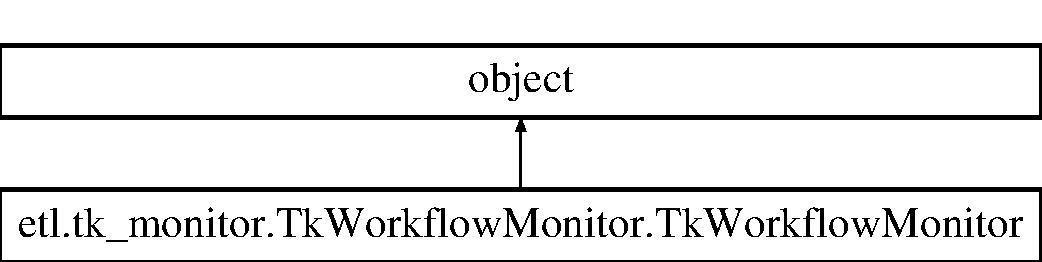
\includegraphics[height=2.000000cm]{classetl_1_1tk__monitor_1_1TkWorkflowMonitor_1_1TkWorkflowMonitor}
\end{center}
\end{figure}
\subsection*{Public Member Functions}
\begin{DoxyCompactItemize}
\item 
def \hyperlink{classetl_1_1tk__monitor_1_1TkWorkflowMonitor_1_1TkWorkflowMonitor_ae3eb503742314535f9f95f6f12f4bce9}{\-\_\-\-\_\-init\-\_\-\-\_\-}
\item 
\hypertarget{classetl_1_1tk__monitor_1_1TkWorkflowMonitor_1_1TkWorkflowMonitor_a6791de02595e3a35f1aa08f9d67dcdbb}{def {\bfseries run\-\_\-gui}}\label{classetl_1_1tk__monitor_1_1TkWorkflowMonitor_1_1TkWorkflowMonitor_a6791de02595e3a35f1aa08f9d67dcdbb}

\end{DoxyCompactItemize}
\subsection*{Public Attributes}
\begin{DoxyCompactItemize}
\item 
\hypertarget{classetl_1_1tk__monitor_1_1TkWorkflowMonitor_1_1TkWorkflowMonitor_a213c1624b03d062e111a639a421e1594}{{\bfseries prc\-\_\-status\-\_\-grid}}\label{classetl_1_1tk__monitor_1_1TkWorkflowMonitor_1_1TkWorkflowMonitor_a213c1624b03d062e111a639a421e1594}

\end{DoxyCompactItemize}


\subsection{Detailed Description}
\begin{DoxyVerb}GUI Application to run, monitor, and trace a workflow\end{DoxyVerb}
 

\subsection{Constructor \& Destructor Documentation}
\hypertarget{classetl_1_1tk__monitor_1_1TkWorkflowMonitor_1_1TkWorkflowMonitor_ae3eb503742314535f9f95f6f12f4bce9}{\index{etl\-::tk\-\_\-monitor\-::\-Tk\-Workflow\-Monitor\-::\-Tk\-Workflow\-Monitor@{etl\-::tk\-\_\-monitor\-::\-Tk\-Workflow\-Monitor\-::\-Tk\-Workflow\-Monitor}!\-\_\-\-\_\-init\-\_\-\-\_\-@{\-\_\-\-\_\-init\-\_\-\-\_\-}}
\index{\-\_\-\-\_\-init\-\_\-\-\_\-@{\-\_\-\-\_\-init\-\_\-\-\_\-}!etl::tk_monitor::TkWorkflowMonitor::TkWorkflowMonitor@{etl\-::tk\-\_\-monitor\-::\-Tk\-Workflow\-Monitor\-::\-Tk\-Workflow\-Monitor}}
\subsubsection[{\-\_\-\-\_\-init\-\_\-\-\_\-}]{\setlength{\rightskip}{0pt plus 5cm}def etl.\-tk\-\_\-monitor.\-Tk\-Workflow\-Monitor.\-Tk\-Workflow\-Monitor.\-\_\-\-\_\-init\-\_\-\-\_\- (
\begin{DoxyParamCaption}
\item[{}]{self, }
\item[{}]{workflow}
\end{DoxyParamCaption}
)}}\label{classetl_1_1tk__monitor_1_1TkWorkflowMonitor_1_1TkWorkflowMonitor_ae3eb503742314535f9f95f6f12f4bce9}
\begin{DoxyVerb}Init

@param workflow: etl.Workflow object with ETL components added/connected
\end{DoxyVerb}
 

The documentation for this class was generated from the following file\-:\begin{DoxyCompactItemize}
\item 
src/etl/tk\-\_\-monitor/Tk\-Workflow\-Monitor.\-py\end{DoxyCompactItemize}

\hypertarget{classetl_1_1WorkflowDataPath_1_1WorkflowDataPath}{\section{etl.\-Workflow\-Data\-Path.\-Workflow\-Data\-Path Class Reference}
\label{classetl_1_1WorkflowDataPath_1_1WorkflowDataPath}\index{etl.\-Workflow\-Data\-Path.\-Workflow\-Data\-Path@{etl.\-Workflow\-Data\-Path.\-Workflow\-Data\-Path}}
}
Inheritance diagram for etl.\-Workflow\-Data\-Path.\-Workflow\-Data\-Path\-:\begin{figure}[H]
\begin{center}
\leavevmode
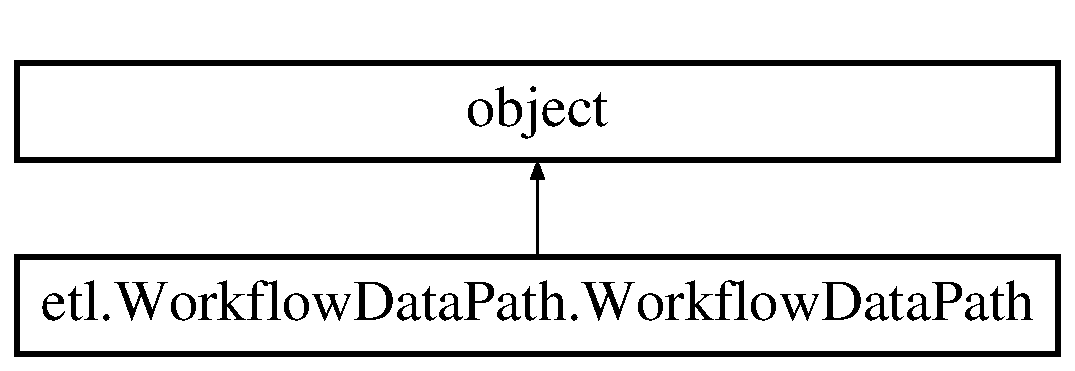
\includegraphics[height=2.000000cm]{classetl_1_1WorkflowDataPath_1_1WorkflowDataPath}
\end{center}
\end{figure}
\subsection*{Public Member Functions}
\begin{DoxyCompactItemize}
\item 
\hypertarget{classetl_1_1WorkflowDataPath_1_1WorkflowDataPath_afae37c9b8563fa47af0c879335140bda}{def {\bfseries \-\_\-\-\_\-init\-\_\-\-\_\-}}\label{classetl_1_1WorkflowDataPath_1_1WorkflowDataPath_afae37c9b8563fa47af0c879335140bda}

\end{DoxyCompactItemize}
\subsection*{Public Attributes}
\begin{DoxyCompactItemize}
\item 
\hypertarget{classetl_1_1WorkflowDataPath_1_1WorkflowDataPath_a9c6118cd7f21966a1c550bbccac086c3}{{\bfseries src\-\_\-prc\-\_\-name}}\label{classetl_1_1WorkflowDataPath_1_1WorkflowDataPath_a9c6118cd7f21966a1c550bbccac086c3}

\item 
\hypertarget{classetl_1_1WorkflowDataPath_1_1WorkflowDataPath_a1ea3fede4a7b02c4c1ff837c69a38b13}{{\bfseries src\-\_\-prc}}\label{classetl_1_1WorkflowDataPath_1_1WorkflowDataPath_a1ea3fede4a7b02c4c1ff837c69a38b13}

\item 
\hypertarget{classetl_1_1WorkflowDataPath_1_1WorkflowDataPath_a50bf171611102cf31af68d7ff1619a7c}{{\bfseries output\-\_\-name}}\label{classetl_1_1WorkflowDataPath_1_1WorkflowDataPath_a50bf171611102cf31af68d7ff1619a7c}

\item 
\hypertarget{classetl_1_1WorkflowDataPath_1_1WorkflowDataPath_a324c55d3e221dcff006a59d2b03a82c6}{{\bfseries output\-\_\-schema}}\label{classetl_1_1WorkflowDataPath_1_1WorkflowDataPath_a324c55d3e221dcff006a59d2b03a82c6}

\item 
\hypertarget{classetl_1_1WorkflowDataPath_1_1WorkflowDataPath_aa96df6d69b6608dbe992bd8ee3497709}{{\bfseries dst\-\_\-prc\-\_\-name}}\label{classetl_1_1WorkflowDataPath_1_1WorkflowDataPath_aa96df6d69b6608dbe992bd8ee3497709}

\item 
\hypertarget{classetl_1_1WorkflowDataPath_1_1WorkflowDataPath_a7d2c1a9dbdbac703062839295c756e86}{{\bfseries input\-\_\-name}}\label{classetl_1_1WorkflowDataPath_1_1WorkflowDataPath_a7d2c1a9dbdbac703062839295c756e86}

\item 
\hypertarget{classetl_1_1WorkflowDataPath_1_1WorkflowDataPath_a3c86bf3a89f3ed12dc850112c5d0f1c1}{{\bfseries input\-\_\-schema}}\label{classetl_1_1WorkflowDataPath_1_1WorkflowDataPath_a3c86bf3a89f3ed12dc850112c5d0f1c1}

\item 
\hypertarget{classetl_1_1WorkflowDataPath_1_1WorkflowDataPath_a056f656eda567abd4f642f512e4cdedf}{{\bfseries dst\-\_\-prc}}\label{classetl_1_1WorkflowDataPath_1_1WorkflowDataPath_a056f656eda567abd4f642f512e4cdedf}

\item 
\hypertarget{classetl_1_1WorkflowDataPath_1_1WorkflowDataPath_af312a99c433a92aa7a17a0468929873b}{{\bfseries dst\-\_\-prc\-\_\-manager}}\label{classetl_1_1WorkflowDataPath_1_1WorkflowDataPath_af312a99c433a92aa7a17a0468929873b}

\end{DoxyCompactItemize}


\subsection{Detailed Description}
\begin{DoxyVerb}Describes a connection between EtlProcessors\end{DoxyVerb}
 

The documentation for this class was generated from the following file\-:\begin{DoxyCompactItemize}
\item 
src/etl/Workflow\-Data\-Path.\-py\end{DoxyCompactItemize}

%--- End generated contents ---

% Index
\newpage
\phantomsection
\addcontentsline{toc}{chapter}{Index}
\printindex

\end{document}
